%%%%%% Run at command line, run
%%%%%% xelatex grad-sample.tex 
%%%%%% for a few times to generate the output pdf file
\documentclass[12pt,oneside,openright,a4paper]{cpe-thai-project}


\usepackage{polyglossia}
\usepackage{titlesec}
\usepackage{multirow}
\usepackage{graphicx}
\usepackage[table,xcdraw]{xcolor}
\setdefaultlanguage{thai}
\setotherlanguage{english}
\newfontfamily\thaifont[Script=Thai,Scale=1.23]{TH Sarabun New}
\defaultfontfeatures{Mapping=tex-text,Scale=1.23,LetterSpace=0.0}
\setmainfont[Scale=1.23,LetterSpace=0,WordSpace=1.0,FakeStretch=1.0,Mapping=tex-text]{TH Sarabun New}
\XeTeXlinebreaklocale "th"	
\XeTeXlinebreakskip = 0pt plus 0pt
\emergencystretch=10pt


%%%%%%%%%%%%%%%%%%%%%%%%%%%%%%%%%%%%%%%%%%%%%%%%%%%%%%%%%%%%%%%%%%%
% Customize below to suit your needs 
% The ones that are optional can be left blank. 
%%%%%%%%%%%%%%%%%%%%%%%%%%%%%%%%%%%%%%%%%%%%%%%%%%%%%%%%%%%%%%%%%%%
% First line of title
\def\disstitleone{Document management system for lawyer}   
% Second line of title
% \def\disstitletwo{Project/Indep title line 2 (optional)}   
% Your first name and lastname
\def\dissauthor{Mr. Kittipat Dechkul}   % 1st member
\def\dissauthortwo{Mr. Choolerk Taebanpakul}   % 2nd member (optional)
\def\dissauthorthree{}   % 2nd member (optional)


% The degree that you're persuing..
\def\dissdegree{Bachelor of Engineering} % Name of the degree
\def\dissdegreeabrev{B.Eng} % Abbreviation of the degree
\def\dissyear{2022}                   % Year of submission
\def\thaidissyear{2565}               % Year of submission (B.E.)

%%%%%%%%%%%%%%%%%%%%%%%%%%%%%%%%%%%%%%%%%%%%
% Your project and independent study committee..
%%%%%%%%%%%%%%%%%%%%%%%%%%%%%%%%%%%%%%%%%%%%
\def\dissadvisor{Asst.Prof. Dr.-Ing Priyakorn Pusawiro}  % Advisor
\def\disscoadvisor{}  % Co-advisor
\def\disscommitteetwo{Asst.Prof. Sanan Srakaew}  % 3rd committee member (optional)
\def\disscommitteethree{Asst.Prof. Suthathip Maneewongvatana, Ph.D.}   % 4th committee member (optional) 
\def\disscommitteefour{Kharittha Jangsamsi, Ph.D.}    % 5th committee member (optional) 

\def\worktype{Project} %%  Project or Independent study
\def\disscredit{3}   %% 3 credits or 6 credits


\def\fieldofstudy{Computer Engineering} 
\def\department{Computer Engineering} 
\def\faculty{Engineering}

\def\thaifieldofstudy{วิศวกรรมคอมพิวเตอร์} 
\def\thaidepartment{วิศวกรรมคอมพิวเตอร์} 
\def\thaifaculty{วิศวกรรมศาสตร์}
 
\def\appendixnames{Appendix} %%% Appendices or Appendix

\def\thaiworktype{ปริญญานิพนธ์} %  Project or research project % 
\def\thaidisstitleone{Document management system for lawyer}
% \def\thaidisstitletwo{หัวข้อปริญญานิพนธ์บรรทัดสอง}
\def\thaidissauthor{นายกิตติภัฎ เดชกุล}
\def\thaidissauthortwo{นายชูฤกษ์ แต่บรรพกุล} %Optional
\def\thaidissauthorthree{} %Optional

\def\thaidissadvisor{รศ.ดร. ปริยกร ปุสวิโร}
%% Leave this empty if you have no co-advisor
% \def\thaidisscoadvisor{นายสุรสิทธิ์ ประคุณหังสิต} %Optional
\def\thaidissdegree{วิศวกรรมศาสตรบัณฑิต}

% Change the line spacing here...
\linespread{1.15}

%%%%%%%%%%%%%%%%%%%%%%%%%%%%%%%%%%%%%%%%%%%%%%%%%%%%%%%%%%%%%%%%
% End of personal customization.  Do not modify from this part 
% to \begin{document} unless you know what you are doing...
%%%%%%%%%%%%%%%%%%%%%%%%%%%%%%%%%%%%%%%%%%%%%%%%%%%%%%%%%%%%%%%%


%%%%%%%%%%%% Dissertation style %%%%%%%%%%%
%\linespread{1.6} % Double-spaced  
%%\oddsidemargin    0.5in
%%\evensidemargin   0.5in
%%%%%%%%%%%%%%%%%%%%%%%%%%%%%%%%%%%%%%%%%%%
%\renewcommand{\subfigtopskip}{10pt}
%\renewcommand{\subfigbottomskip}{-5pt} 
%\renewcommand{\subfigcapskip}{-6pt} %vertical space between caption
%                                    %and figure.
%\renewcommand{\subfigcapmargin}{0pt}

\renewcommand{\topfraction}{0.85}
\renewcommand{\textfraction}{0.1}

\newtheorem{theorem}{Theorem}
\newtheorem{lemma}{Lemma}
\newtheorem{corollary}{Corollary}

\def\QED{\mbox{\rule[0pt]{1.5ex}{1.5ex}}}
\def\proof{\noindent\hspace{2em}{\itshape Proof: }}
\def\endproof{\hspace*{\fill}~\QED\par\endtrivlist\unskip}
%\newenvironment{proof}{{\sc Proof:}}{~\hfill \blacksquare}
%% The hyperref package redefines the \appendix. This one 
%% is from the dissertation.cls
%\def\appendix#1{\iffirstappendix \appendixcover \firstappendixfalse \fi \chapter{#1}}
%\renewcommand{\arraystretch}{0.8}
%%%%%%%%%%%%%%%%%%%%%%%%%%%%%%%%%%%%%%%%%%%%%%%%%%%%%%%%%%%%%%%%
%%%%%%%%%%%%%%%%%%%%%%%%%%%%%%%%%%%%%%%%%%%%%%%%%%%%%%%%%%%%%%%%

\usepackage{ragged2e}
\begin{document}

\pdfstringdefDisableCommands{%
\let\MakeUppercase\relax
}

\begin{center}
  
\includegraphics[width=2.8cm]{logo02.jpg}
\end{center}
\vspace*{-1cm}

\maketitlepage
\makesignaturepage 

%%%%%%%%%%%%%%%%%%%%%%%%%%%%%%%%%%%%%%%%%%%%%%%%%%%%%%%%%%%%%%
%%%%%%%%%%%%%%%%%%%%%% English abstract %%%%%%%%%%%%%%%%%%%%%%%
%%%%%%%%%%%%%%%%%%%%%%%%%%%%%%%%%%%%%%%%%%%%%%%%%%%%%%%%%%%%%%
\abstract

English abstract 

\begin{flushleft}
\begin{tabular*}{\textwidth}{@{}lp{0.8\textwidth}}
\textbf{Keywords}: & Web application / (DMS) Document Management System / (OCR) Optical Character Recognition
\end{tabular*}
\end{flushleft}
\endabstract

%%%%%%%%%%%%%%%%%%%%%%%%%%%%%%%%%%%%%%%%%%%%%%%%%%%%%%%%%%%%%%
%%%%%%%%%% Thai abstract here %%%%%%%%%%%%%%%%%%%%%%%%%%%%%%%%%
%%%%%%%%%%%%%%%%%%%%%%%%%%%%%%%%%%%%%%%%%%%%%%%%%%%%%%%%%%%%%%
% {\newfontfamily\thaifont{TH Sarabun New:script=thai}[Scale=1.3]
% \XeTeXlinebreaklocale "th_TH"	
% \thaifont
\thaiabstract

\hspace*{1cm} ในปัจจุบันได้เกิดคดีความต่าง ๆ มากมายทั้งคดีออาชญากรรม คดียาเสพติด หรือคดีทางการเมือง และในบางคดีนั้นผู้ที่ถูกดำเนินคดีมักจะถูกกลั่นแกล้งผ่านทางกฎหมายหรือไม่ได้รับความเป็นธรรมโดยเฉพาะคดีที่เกี่ยวข้องกับการเมือง โดยจะมีทั้งเยาวชน นักศึกษามหาวิทยาลัย และประชาชนทั่วไป ซึ่งถ้าจะไปจ้างทนายส่วนตัวก็จะต้องเสียทั้งเงิน เสียทั้งเวลา ดังนั้นจึงมีองค์กรที่ไม่แสวงหาผลกำไร ที่จะจัดตั้งทนายขึ้นมา เพื่อที่จะมาช่วยเหลือ ผู้ที่ถูกดำเนินคดีทางการเมืองเหล่านี้ ซึ่งในปัจจุบันก็จะมีองค์กรที่คอยให้ความช่วยเหลือ และเป็นองค์กรไม่แสวงผลกำไร โดยจะเข้ามามีบทบาทในการช่วยเหลือผู้ที่ถูกดำเนินคดี แต่จำนวนของทนายที่จะคอยให้ความช่วยเหลือนั้นมีไม่เพียงพอ ประกอบกับจำนวนของผู้ที่ถูกดำเนินคดีที่มีมากขึ้นเรื่อย ๆ โดยจะเห็นว่าทนาย 1 คนนั้นมีความจำเป็นที่จะต้องรับผิดชอบคดีความมากกว่า 1 คดี และต้องรับทำคดีมากกว่า 1 คน อีกทั้งยังต้องจัดการเอกสารจำนวนมาก จึงทำให้พบปัญหาในการจัดเก็บเอกสาร หรือรูปภาพอยู่เสมอ โดยเฉพาะในบางคดีที่ใช้ระยะเวลานาน จนอาจจะมีการหลงลืมที่อยู่ในการจัดเก็บเอกสารได้ \\
\hspace*{1cm} ด้วยเหตุเหล่านี้ทางคณะผู้จัดทำได้เล็งเห็นถึงปัญหาดังกล่าว คณะผู้จัดทำจึงต้องการที่จะพัฒนาเว็บแอปพลิเคชันเพื่อใช้ในการจัดการเอกสารต่าง ๆ ของทนาย หรือเรียกสั่น ๆ ว่า D-Law โดยสามารถจัดเก็บเอกสาร ตามรายบุคคลหรือตามเคสแต่ละคดีได้ และยังสามารถนำเอกสารบางส่วนที่เป็นประโยชน์ต่อสาธารณะมาเผยแพร่ ให้บุคคลทั่วไปสามารถดาวน์โหลดและติดตามคดีเหล่านั้นได้ อีกทั้งทางคณะผู้จัดทำจะนำข้อมูลต่าง ๆ ที่มีความน่าสนใจมาจัดทำให้อยู่ในรูปแบบของแผนที่จำลองหรือแผนภูมิในรูปแบบต่าง ๆ เพื่อที่จะให้บุคคลทั่วไปได้ศึกษาข้อมูล พร้อมทั้งเข้าถึงสถานการณ์ทางด้านกฎหมายและคดีทางการเมืองของประเทศไทยในปัจจุบัน


\begin{flushleft}
\begin{tabular*}{\textwidth}{@{}lp{0.8\textwidth}}
 & \\

\textbf{คำสำคัญ}: & เว็บแอปพลิเคชัน / ระบบจัดการเอกสาร / (OCR) Optical Character Recognition
\end{tabular*}
\end{flushleft}
\endabstract

%}

%%%%%%%%%%%%%%%%%%%%%%%%%%%%%%%%%%%%%%%%%%%%%%%%%%%%%%%%%%%%
%%%%%%%%%%%%%%%%%%%%%%% Acknowledgments %%%%%%%%%%%%%%%%%%%%
%%%%%%%%%%%%%%%%%%%%%%%%%%%%%%%%%%%%%%%%%%%%%%%%%%%%%%%%%%%%
\preface
\hspace*{1cm} การจัดทำปริญญานิพนธ์ในครั้งนี้สำเร็จลุล่วงด้วยดีเพราะได้ความช่วยเหลือจากจาก รศ.ดร. ปริยกร ปุสวิโร ซึ่งเป็นอาจารย์ที่ปรึกษาซึ่งได้ความกรุณาสละเวลามาให้คำปรึกษาหรือคำแนะนำอันเป็นประโชน์ในการจำทำปริญญานิพนธ์ อีกทั้งยังให้ความช่วยเหลือในตลอดระยะเวลาในการจำทำปริญญานิพนธ์ในครั้งนี้ ทางคณะผู้จัดทำปริญญานิพนธ์จึงขอกราบขอบพระคุณอาจารย์เป็นอย่างยิ่ง \\
\hspace*{1cm}ขอขอบพระคุณ ทนายพี่เป๋า ทนายประจำโครงการอินเทอร์เน็ตเพื่อกฎหมายประชาชน และทนายพี่แอน ทนายประจำศูนย์ทนายความเพื่อสิทธิมนุษยชน ที่ได้สละเวลาอันมีค่ามาให้คำแนะนำ ความรู้เฉพาะด้าน ข้อมูลเกี่ยวกับกฎหมาย และขั้นตอนทางกฎหมาย อีกทั้งยังคอยเป็นที่ปรึกษาและให้ความช่วยเหลือตลอดเวลาในการทำปริญญานิพนธ์นี้ \\
\hspace*{1cm}ขอขอบพระคุณคณะกรรมการที่ได้สละเวลามาร่วมเป็นกรรมการในการตรวจสอบปริญญานิพนธ์ชิ้นนี้ รวมถึงให้ข้อคิดเห็น ชี้แนะต่าง ๆ ที่เป็นประโยชน์แก่การจัดทำปริญญานิพนธ์นี้ \\
\hspace*{1cm}ท้ายที่สุดนี้ ปริญญานิพนธ์นี้จะสำเร็จลุล่วงไม่ได้เลยถ้าหาก ไม่มีบิดา มารดา เพื่อน และรุ่นพี่ในภาควิชาวิศวกรรมคอมพิวเตอร์ที่คอยแนะนำ ให้ความช่วยเหลือ สนับสนุน อีกทั้งยังคอยเป็นกำลังใจให้กับคณะผู้จัดทำอยู่เสมอมา ทางคณะู้จัดทำหวังเป็นอย่างยิ่งว่าปริญญานิพนธ์นี้จะก่อประโยชน์แก่ทางศูนย์ทนาย และผู้ที่สนใจในแอปพลิเคชั่นนี้ไม่มากก็น้อย \\
\hspace*{\fill} คณะผู้จัดทำปริญญานิพนธ์

%%%%%%%%%%%%%%%%%%%%%%%%%%%%%%%%%%%%%%%%%%%%%%%%%%%%%%%%%%%%%
%%%%%%%%%%%%%%%% ToC, List of figures/tables %%%%%%%%%%%%%%%%
%%%%%%%%%%%%%%%%%%%%%%%%%%%%%%%%%%%%%%%%%%%%%%%%%%%%%%%%%%%%%
% The three commands below automatically generate the table 
% of content, list of tables and list of figures
\tableofcontents                    
\listoftables
\listoffigures                      

%%%%%%%%%%%%%%%%%%%%%%%%%%%%%%%%%%%%%%%%%%%%%%%%%%%%%%%%%%%%%%
%%%%%%%%%%%%%%%%%%%%% List of symbols page %%%%%%%%%%%%%%%%%%%
%%%%%%%%%%%%%%%%%%%%%%%%%%%%%%%%%%%%%%%%%%%%%%%%%%%%%%%%%%%%%%
% You have to add this manually..
\listofsymbols
\begin{flushleft}
\begin{tabular}{@{}p{0.07\textwidth}p{0.7\textwidth}p{0.1\textwidth}}
\textbf{SYMBOL}  & & \textbf{UNIT} \\[0.2cm]
% $\alpha$ & Test variable\hfill & m$^2$ \\
% $\lambda$ & Interarival rate\hfill &  jobs/second\\
% $\mu$ & Service rate\hfill & jobs/second\\
\end{tabular}
\end{flushleft}
%%%%%%%%%%%%%%%%%%%%%%%%%%%%%%%%%%%%%%%%%%%%%%%%%%%%%%%%%%%%%%
%%%%%%%%%%%%%%%%%%%%% List of vocabs & terms %%%%%%%%%%%%%%%%%
%%%%%%%%%%%%%%%%%%%%%%%%%%%%%%%%%%%%%%%%%%%%%%%%%%%%%%%%%%%%%%
% You also have to add this manually..
\listofvocab
\begin{flushleft}
\begin{tabular}{@{}p{1in}@{=\extracolsep{0.5in}}l}
  OCR &  Optical Character Recognition \\
  UX &  User Experience \\
  UI &  User Interface \\
  API &  Application Program Interface \\
\end{tabular}
\end{flushleft}

%\setlength{\parskip}{1.2mm}

%%%%%%%%%%%%%%%%%%%%%%%%%%%%%%%%%%%%%%%%%%%%%%%%%%%%%%%%%%%%%%%
%%%%%%%%%%%%%%%%%%%%%%%% Main body %%%%%%%%%%%%%%%%%%%%%%%%%%%%
%%%%%%%%%%%%%%%%%%%%%%%%%%%%%%%%%%%%%%%%%%%%%%%%%%%%%%%%%%%%%%%


\chapter{บทนำ}

\section{ที่มาและความสำคัญ}

\hspace*{1cm} ในปัจจุบันได้เกิดคดีความต่าง ๆ มากมายทั้งคดีออาชญากรรม คดียาเสพติด หรือคดีทางการเมือง และในบางคดีนั้นผู้ที่ถูกดำเนินคดีมักจะถูกกลั่นแกล้งผ่านทางกฎหมายหรือไม่ได้รับความเป็นธรรมโดยเฉพาะคดีที่เกี่ยวข้องกับการเมือง โดยจะมีทั้งเยาวชน นักศึกษามหาวิทยาลัย และประชาชนทั่วไป ซึ่งถ้าจะไปจ้างทนายส่วนตัวก็จะต้องเสียทั้งเงิน เสียทั้งเวลา ดังนั้นจึงมีองค์กรที่ไม่แสวงหาผลกำไร ที่จะจัดตั้งทนายขึ้นมา เพื่อที่จะมาช่วยเหลือ ผู้ที่ถูกดำเนินคดีทางการเมืองเหล่านี้ ซึ่งในปัจจุบันก็จะมีองค์กรที่คอยให้ความช่วยเหลือ และเป็นองค์กรไม่แสวงผลกำไร ซึ่งมีจำนวนทั้งสิ้น 2 องค์กรคือ โครงการอินเทอร์เน็ตเพื่อกฎหมายประชาชนซึ่งมีชื่อว่า I-Law และ ศูนย์ทนายความเพื่อสิทธิมนุษยชนหรือ TLHR โดยองค์กรไม่แสวงผลกำไรนี้ได้เข้ามามีบทบาท ทำให้ผู้ที่ถูกดำเนินคดีทางการเมืองจำนวนมากต่างเข้ามาติดต่อเพื่อขอความช่วยเหลือ และในทางกลับกันจำนวนของทนายที่คอยให้ความช่วยเหลือผู้ที่ถูกดำเนินคดีนั้นมีจำนวนเท่าเดิม และมีแนวโน้มที่จะมีผู้ที่ถูกดำเนินคดีมากขึ้นเรื่อย ๆ  จากที่กล่าวมาข้างต้นจะเห็นได้ว่าทนาย 1 คนนั้นมีความจำเป็นที่จะต้องรับผิดชอบคดีความมากกว่า 1 คดี และต้องรับทำคดีมากกว่า 1 คน อีกทั้งยังต้องจัดการเอกสารจำนวนมาก จึงทำให้พบปัญหาในการจัดเก็บเอกสาร หรือรูปภาพอยู่เสมอ โดยเฉพาะในบางคดีที่ใช้ระยะเวลานาน จนอาจจะมีการหลงลืมที่อยู่ในการจัดเก็บเอกสารได้ \\
\hspace*{1cm} ด้วยเหตุเหล่านี้ทางคณะผู้จัดทำได้เล็งเห็นถึงปัญหาดังกล่าว คณะผู้จัดทำจึงต้องการที่จะพัฒนาเว็บแอปพลิเคชันเพื่อใช้ในการจัดการเอกสารต่าง ๆ ของทนาย หรือมีชื่อเรียกว่า D-Law โดยสามารถจัดเก็บเอกสาร ตามรายบุคคลหรือตามเคสแต่ละคดีได้ และยังสามารถนำเอกสารบางส่วนที่เป็นประโยชน์ต่อสาธารณะมาเผยแพร่ ให้บุคคลทั่วไปสามารถดาวน์โหลดและติดตามคดีเหล่านั้นได้ อีกทั้งทางคณะผู้จัดทำจะนำข้อมูลต่าง ๆ ที่มีความน่าสนใจมาจัดทำให้อยู่ในรูปแบบของแผนที่จำลองหรือแผนภูมิในรูปแบบต่าง ๆ เพื่อที่จะให้บุคคลทั่วไปได้ศึกษาข้อมูล พร้อมทั้งเข้าถึงสถานการณ์ทางด้านกฎหมายและคดีทางการเมืองของประเทศไทยในปัจจุบัน

\section{วัตถุประสงค์}
\begin{enumerate}
  \item เพื่อศึกษาระบบในการบริหารจัดการเอกสาร การติดตาม และขั้นตอนการดำเนินคดีต่าง ๆ ของสำนักทนายความ
  \item เพื่อออกแบบฐานข้อมูล ให้เหมาะสมหรือสอดคล้องกับการค้นหาและจัดเก็บเอกสารอิเล็กทอนิค
  \item เพื่อพัฒนาเว็บแอปพลิเคชันที่ใช้ในการบริหารจัดการเอกสาร
  \item เพื่อสร้างช่องทางเข้าถึงข้อมูลเบื้องต้นอย่างง่ายให้กับทนายความและลูกความ
\end{enumerate}

\section{ขอบเขตและข้อจำกัดของปริญญานิพนธ์}
\hspace*{1cm}เว็บแอปพลิเคชัน Document management system for lawyer สามารถทำงานได้เมื่อมีอินเทอร์เน็ตเท่านั้น และสามารถทำงานได้บนคอมพิวเตอร์ผ่านเว็บเบราว์เซอร์เท่านั้นอาทิเช่น Google Chrome, Safari หรือ Microsoft Edge อีกทั้งข้อมูลที่นำมาใช้ในปริญญานิพนธ์นี้จะเป็นข้อมูลจริงที่ถูกเผยแพร่ผ่านเว็บไซต์ของศาลยุติธรรมซึ่งข้อมูลนี้ทุกคนสามารถเข้าถึงข้อมูลเหล่านี้ได้ และอีกส่วนหนึ่งเป็นข้อมูลเอกสารที่ได้ความยินยอมจากเจ้าของคดีและทนายให้สามารถเผยแพร่และเป็นตัวอย่างในปริญญานิพนธ์นี้เท่านั้น

\section{เนื้อหาทางวิศวกรรมที่เป็นต้นฉบับ}
\hspace*{1cm}โครงงานนี้พัฒนาขึ้นจากการใช้ความรู้ในด้านการออกแบบฐานข้อมูล ความรู้ในการพัฒนาเว็บแอปพลิเคชัน รวมไปถึงความรู้ทางด้านวิศวกรรมซอฟต์แวร์ ซึ่งไม่ว่าจะเป็นการออกแบบ UML diagram ต่าง ๆ การวางแผนการทำงาน การพัฒนาซอฟต์แวร์ในรูปแบบของ Waterfall การใช้ Kanbann เพื่อช่วยในการจัดการการทำงาน มาใช้เพื่อสร้างเป็นเว็บแอปพลิเคชันสำหรับจัดการเอกสารของทนาย โดยมีการใช้ Elasticsearch ในการค้นหาเอกสาร และใช้ Gin framework ที่ใช้ภาษา Go language มาจัดการส่วนของการประมวณผล สุดท้ายได้นำ NextJs Framework ซึ่งใช้ภาษา Typescript , component framework และ CSS framework มาใช้ในการ แสดงข้อมูลที่ถูกประมวลผลแล้ว 

\newpage
\section{ขั้นตอนการทํางานและระยะเวลาการดําเนินงาน}
\begin{enumerate}
  \item{กำหนดหัวข้อโครงงานและปรึกษาอาจารที่ปรึกษา} 
  \item{รวบรวมข้อมูลที่เกี่ยวข้องกับโครงงาน}
  \item{ศึกษาเครื่องมือที่ใช้ในการทำโครงงาน}
  \item{ศึกษาค้นคว้าและเก็บรวบรวมข้อมูลที่ใช้ในการทำโครงการ}
  \item{จัดทำข้อเสนอโครงการ}
  \item{จัดทำรูปเล่มปริญญานิพนธ์ประจำภาคการศึกษาที่ 1/2565}
  \item{ออกแบบ โครงสร้าง UX/UI และฐานข้อมูล}
  \begin{itemize}
        \item{ออกแบบ และจัดวาง flow ของระบบ}
        \item{ออกแบบ UX/UI ของเว็บแอปพลิเคชัน}
    \end{itemize}
\item{ทดสอบเทคโนโลยี และทฤษฎีที่นำมาใช้ การพัฒนา Web  Application}
\item{พัฒนาเว็บแอปพลิเคชัน}
    \begin{itemize}
        \item{ศึกษาและพัฒนา Frontend ด้วย NextJS (Javascript)}
        \item{ศึกษาและพัฒนา Backend ด้วยภาษา Go}
        \item{ศึกษาและพัฒนาฐานข้อมูลด้วย PostgreSQL, Elasticsearch}
    \end{itemize}
  \item{นำเสนอปริญญานิพนธ์ประจำภาคการศึกษาที่ 1/2565}
  \item{พัฒนาเว็บแอปพลิเคชัน (ต่อจากภาคเรียนที่ 1)}
  \item{ทดสอบเว็บแอปพลิเคชัน (ต่อจากภาคเรียนที่ 1)}
  \item{ปรับปรุงและแก้ไขเว็บแอปพลิเคชัน}
  \item{ทดสอบการใช้งานจริง}
  \item{จัดทำรูปเล่มปริญญานิพนธ์ประจำภาคการศึกษาที่ 2/2565}
  \item{นำเสนอปริญญานิพนธ์ประจำภาคการศึกษาที่ 2/2565}
\end{enumerate}
\hspace*{1cm}จากขั้นตอนการทำงานทั้งหมดที่กล่าวมา สามารถแสดงผลเวลาในการดำเนินงาน ในรูปแบบของแผนภูมิแกนต์ (Gantt chart) ได้ดังตารางที่ \ref{tbl:working1} และตารางที่ \ref{tbl:working2} ดังนี้

\begin{table}[!ht]
    \resizebox{\columnwidth}{!}{%
    \begin{tabular}{|llllllllllllllllllllll|}
    \hline
    \multicolumn{22}{|c|}{ตารางดำเนินงาน ภาคการศึกษาที่ 1/2565} \\ \hline
    \multicolumn{1}{|c|}{} &
      \multicolumn{1}{c|}{} &
      \multicolumn{4}{c|}{สิงหาคม} &
      \multicolumn{4}{c|}{กันยายน} &
      \multicolumn{4}{c|}{ตุลาคม} &
      \multicolumn{4}{c|}{พฤศจิกายน} &
      \multicolumn{4}{c|}{ธันวาคม} \\ \cline{3-22} 
    \multicolumn{1}{|c|}{\multirow{-2}{*}{ที่}} &
      \multicolumn{1}{c|}{\multirow{-2}{*}{หัวข้อ}} &
      \multicolumn{1}{c|}{1} &
      \multicolumn{1}{c|}{2} &
      \multicolumn{1}{c|}{3} &
      \multicolumn{1}{c|}{4} &
      \multicolumn{1}{c|}{1} &
      \multicolumn{1}{c|}{2} &
      \multicolumn{1}{c|}{3} &
      \multicolumn{1}{c|}{4} &
      \multicolumn{1}{c|}{1} &
      \multicolumn{1}{c|}{2} &
      \multicolumn{1}{c|}{3} &
      \multicolumn{1}{c|}{4} &
      \multicolumn{1}{c|}{1} &
      \multicolumn{1}{c|}{2} &
      \multicolumn{1}{c|}{3} &
      \multicolumn{1}{c|}{4} &
      \multicolumn{1}{c|}{1} &
      \multicolumn{1}{c|}{2} &
      \multicolumn{1}{c|}{3} &
      \multicolumn{1}{c|}{4} \\ \hline
    \multicolumn{1}{|l|}{1} &
      \multicolumn{1}{l|}{กำหนดหัวข้อโครงงานและปรึกษาอาจารที่ปรึกษา} &
      \multicolumn{1}{l|}{\cellcolor[HTML]{FFCE93}} &
      \multicolumn{1}{l|}{\cellcolor[HTML]{FFCE93}} &
      \multicolumn{1}{l|}{} &
      \multicolumn{1}{l|}{} &
      \multicolumn{1}{l|}{} &
      \multicolumn{1}{l|}{} &
      \multicolumn{1}{l|}{} &
      \multicolumn{1}{l|}{} &
      \multicolumn{1}{l|}{} &
      \multicolumn{1}{l|}{} &
      \multicolumn{1}{l|}{} &
      \multicolumn{1}{l|}{} &
      \multicolumn{1}{l|}{} &
      \multicolumn{1}{l|}{} &
      \multicolumn{1}{l|}{} &
      \multicolumn{1}{l|}{} &
      \multicolumn{1}{l|}{} &
      \multicolumn{1}{l|}{} &
      \multicolumn{1}{l|}{} &
       \\ \hline
    \multicolumn{1}{|l|}{2} &
      \multicolumn{1}{l|}{รวบรวมข้อมูลที่เกี่ยวข้องกับโครงงาน} &
      \multicolumn{1}{l|}{} &
      \multicolumn{1}{l|}{} &
      \multicolumn{1}{l|}{\cellcolor[HTML]{FFCE93}} &
      \multicolumn{1}{l|}{\cellcolor[HTML]{FFCE93}} &
      \multicolumn{1}{l|}{} &
      \multicolumn{1}{l|}{} &
      \multicolumn{1}{l|}{} &
      \multicolumn{1}{l|}{} &
      \multicolumn{1}{l|}{} &
      \multicolumn{1}{l|}{} &
      \multicolumn{1}{l|}{} &
      \multicolumn{1}{l|}{} &
      \multicolumn{1}{l|}{} &
      \multicolumn{1}{l|}{} &
      \multicolumn{1}{l|}{} &
      \multicolumn{1}{l|}{} &
      \multicolumn{1}{l|}{} &
      \multicolumn{1}{l|}{} &
      \multicolumn{1}{l|}{} &
       \\ \hline
    \multicolumn{1}{|l|}{3} &
      \multicolumn{1}{l|}{ศึกษาเครื่องมือที่ใช้ในการทำโครงงาน} &
      \multicolumn{1}{l|}{} &
      \multicolumn{1}{l|}{} &
      \multicolumn{1}{l|}{\cellcolor[HTML]{FFCE93}} &
      \multicolumn{1}{l|}{\cellcolor[HTML]{FFCE93}} &
      \multicolumn{1}{l|}{} &
      \multicolumn{1}{l|}{} &
      \multicolumn{1}{l|}{} &
      \multicolumn{1}{l|}{} &
      \multicolumn{1}{l|}{} &
      \multicolumn{1}{l|}{} &
      \multicolumn{1}{l|}{} &
      \multicolumn{1}{l|}{} &
      \multicolumn{1}{l|}{} &
      \multicolumn{1}{l|}{} &
      \multicolumn{1}{l|}{} &
      \multicolumn{1}{l|}{} &
      \multicolumn{1}{l|}{} &
      \multicolumn{1}{l|}{} &
      \multicolumn{1}{l|}{} &
       \\ \hline
    \multicolumn{1}{|l|}{4} &
      \multicolumn{1}{l|}{ศึกษาค้นคว้าและเก็บรวบรวมข้อมูลที่ใช้ในการทำโครงการ} &
      \multicolumn{1}{l|}{} &
      \multicolumn{1}{l|}{} &
      \multicolumn{1}{l|}{\cellcolor[HTML]{FFCE93}} &
      \multicolumn{1}{l|}{\cellcolor[HTML]{FFCE93}} &
      \multicolumn{1}{l|}{} &
      \multicolumn{1}{l|}{} &
      \multicolumn{1}{l|}{} &
      \multicolumn{1}{l|}{} &
      \multicolumn{1}{l|}{} &
      \multicolumn{1}{l|}{} &
      \multicolumn{1}{l|}{} &
      \multicolumn{1}{l|}{} &
      \multicolumn{1}{l|}{} &
      \multicolumn{1}{l|}{} &
      \multicolumn{1}{l|}{} &
      \multicolumn{1}{l|}{} &
      \multicolumn{1}{l|}{} &
      \multicolumn{1}{l|}{} &
      \multicolumn{1}{l|}{} &
       \\ \hline
    \multicolumn{1}{|l|}{5} &
      \multicolumn{1}{l|}{จัดทำข้อเสนอโครงการ} &
      \multicolumn{1}{l|}{} &
      \multicolumn{1}{l|}{} &
      \multicolumn{1}{l|}{} &
      \multicolumn{1}{l|}{} &
      \multicolumn{1}{l|}{\cellcolor[HTML]{FFCE93}} &
      \multicolumn{1}{l|}{} &
      \multicolumn{1}{l|}{} &
      \multicolumn{1}{l|}{} &
      \multicolumn{1}{l|}{} &
      \multicolumn{1}{l|}{} &
      \multicolumn{1}{l|}{} &
      \multicolumn{1}{l|}{} &
      \multicolumn{1}{l|}{} &
      \multicolumn{1}{l|}{} &
      \multicolumn{1}{l|}{} &
      \multicolumn{1}{l|}{} &
      \multicolumn{1}{l|}{} &
      \multicolumn{1}{l|}{} &
      \multicolumn{1}{l|}{} &
       \\ \hline
    \multicolumn{1}{|l|}{6} &
      \multicolumn{1}{l|}{จัดทำรายงาน   3 บทแรก} &
      \multicolumn{1}{l|}{} &
      \multicolumn{1}{l|}{} &
      \multicolumn{1}{l|}{} &
      \multicolumn{1}{l|}{} &
      \multicolumn{1}{l|}{\cellcolor[HTML]{FFCE93}} &
      \multicolumn{1}{l|}{\cellcolor[HTML]{FFCE93}} &
      \multicolumn{1}{l|}{\cellcolor[HTML]{FFCE93}} &
      \multicolumn{1}{l|}{\cellcolor[HTML]{FFCE93}} &
      \multicolumn{1}{l|}{\cellcolor[HTML]{FFCE93}} &
      \multicolumn{1}{l|}{\cellcolor[HTML]{FFCE93}} &
      \multicolumn{1}{l|}{\cellcolor[HTML]{FFCE93}} &
      \multicolumn{1}{l|}{\cellcolor[HTML]{FFCE93}} &
      \multicolumn{1}{l|}{\cellcolor[HTML]{FFCE93}} &
      \multicolumn{1}{l|}{\cellcolor[HTML]{FFCE93}} &
      \multicolumn{1}{l|}{\cellcolor[HTML]{FFCE93}} &
      \multicolumn{1}{l|}{} &
      \multicolumn{1}{l|}{} &
      \multicolumn{1}{l|}{} &
      \multicolumn{1}{l|}{} &
       \\ \hline
    \multicolumn{1}{|l|}{7} &
      \multicolumn{1}{l|}{ออกแบบโครงสร้าง UX/UI และฐานข้อมูล} &
      \multicolumn{1}{l|}{} &
      \multicolumn{1}{l|}{} &
      \multicolumn{1}{l|}{} &
      \multicolumn{1}{l|}{} &
      \multicolumn{1}{l|}{} &
      \multicolumn{1}{l|}{\cellcolor[HTML]{FFCE93}} &
      \multicolumn{1}{l|}{\cellcolor[HTML]{FFCE93}} &
      \multicolumn{1}{l|}{\cellcolor[HTML]{FFCE93}} &
      \multicolumn{1}{l|}{\cellcolor[HTML]{FFCE93}} &
      \multicolumn{1}{l|}{\cellcolor[HTML]{FFCE93}} &
      \multicolumn{1}{l|}{\cellcolor[HTML]{FFCE93}} &
      \multicolumn{1}{l|}{\cellcolor[HTML]{FFCE93}} &
      \multicolumn{1}{l|}{\cellcolor[HTML]{FFCE93}} &
      \multicolumn{1}{l|}{\cellcolor[HTML]{FFCE93}} &
      \multicolumn{1}{l|}{\cellcolor[HTML]{FFCE93}} &
      \multicolumn{1}{l|}{\cellcolor[HTML]{FFCE93}} &
      \multicolumn{1}{l|}{\cellcolor[HTML]{FFCE93}} &
      \multicolumn{1}{l|}{\cellcolor[HTML]{FFCE93}} &
      \multicolumn{1}{l|}{\cellcolor[HTML]{FFCE93}} &
      \cellcolor[HTML]{FFCE93} \\ \hline
    \multicolumn{1}{|l|}{8} &
      \multicolumn{1}{l|}{ทดสอบเทคโนโลยี และทฤษฎีที่นำมาใช้ในการพัฒนาเว็บแอปพลิเคชัน} &
      \multicolumn{1}{l|}{} &
      \multicolumn{1}{l|}{} &
      \multicolumn{1}{l|}{} &
      \multicolumn{1}{l|}{} &
      \multicolumn{1}{l|}{} &
      \multicolumn{1}{l|}{\cellcolor[HTML]{FFCE93}} &
      \multicolumn{1}{l|}{\cellcolor[HTML]{FFCE93}} &
      \multicolumn{1}{l|}{\cellcolor[HTML]{FFCE93}} &
      \multicolumn{1}{l|}{\cellcolor[HTML]{FFCE93}} &
      \multicolumn{1}{l|}{\cellcolor[HTML]{FFCE93}} &
      \multicolumn{1}{l|}{\cellcolor[HTML]{FFCE93}} &
      \multicolumn{1}{l|}{\cellcolor[HTML]{FFCE93}} &
      \multicolumn{1}{l|}{\cellcolor[HTML]{FFCE93}} &
      \multicolumn{1}{l|}{\cellcolor[HTML]{FFCE93}} &
      \multicolumn{1}{l|}{\cellcolor[HTML]{FFCE93}} &
      \multicolumn{1}{l|}{\cellcolor[HTML]{FFCE93}} &
      \multicolumn{1}{l|}{\cellcolor[HTML]{FFCE93}} &
      \multicolumn{1}{l|}{\cellcolor[HTML]{FFCE93}} &
      \multicolumn{1}{l|}{\cellcolor[HTML]{FFCE93}} &
      \cellcolor[HTML]{FFCE93} \\ \hline
    \multicolumn{1}{|l|}{9} &
      \multicolumn{1}{l|}{พัฒนาเว็บแอปพลิเคชัน} &
      \multicolumn{1}{l|}{} &
      \multicolumn{1}{l|}{} &
      \multicolumn{1}{l|}{} &
      \multicolumn{1}{l|}{} &
      \multicolumn{1}{l|}{} &
      \multicolumn{1}{l|}{\cellcolor[HTML]{FFCE93}} &
      \multicolumn{1}{l|}{\cellcolor[HTML]{FFCE93}} &
      \multicolumn{1}{l|}{\cellcolor[HTML]{FFCE93}} &
      \multicolumn{1}{l|}{\cellcolor[HTML]{FFCE93}} &
      \multicolumn{1}{l|}{\cellcolor[HTML]{FFCE93}} &
      \multicolumn{1}{l|}{\cellcolor[HTML]{FFCE93}} &
      \multicolumn{1}{l|}{\cellcolor[HTML]{FFCE93}} &
      \multicolumn{1}{l|}{\cellcolor[HTML]{FFCE93}} &
      \multicolumn{1}{l|}{\cellcolor[HTML]{FFCE93}} &
      \multicolumn{1}{l|}{\cellcolor[HTML]{FFCE93}} &
      \multicolumn{1}{l|}{\cellcolor[HTML]{FFCE93}} &
      \multicolumn{1}{l|}{\cellcolor[HTML]{FFCE93}} &
      \multicolumn{1}{l|}{\cellcolor[HTML]{FFCE93}} &
      \multicolumn{1}{l|}{\cellcolor[HTML]{FFCE93}} &
      \cellcolor[HTML]{FFCE93} \\ \hline
    \multicolumn{1}{|l|}{10} &
      \multicolumn{1}{l|}{นำเสนอรายงาน   3 บทแรก} &
      \multicolumn{1}{l|}{} &
      \multicolumn{1}{l|}{} &
      \multicolumn{1}{l|}{} &
      \multicolumn{1}{l|}{} &
      \multicolumn{1}{l|}{} &
      \multicolumn{1}{l|}{} &
      \multicolumn{1}{l|}{} &
      \multicolumn{1}{l|}{} &
      \multicolumn{1}{l|}{} &
      \multicolumn{1}{l|}{} &
      \multicolumn{1}{l|}{} &
      \multicolumn{1}{l|}{} &
      \multicolumn{1}{l|}{} &
      \multicolumn{1}{l|}{} &
      \multicolumn{1}{l|}{} &
      \multicolumn{1}{l|}{} &
      \multicolumn{1}{l|}{\cellcolor[HTML]{FFCE93}} &
      \multicolumn{1}{l|}{} &
      \multicolumn{1}{l|}{} &
       \\ \hline
    \end{tabular}%
    }
    \caption{\centering  ตารางแสดงเวลาดำเนินงานของภาคการเรียนที่ 1/2565} \label{tbl:working1}
\end{table}

% Please add the following required packages to your document preamble:
% \usepackage{multirow}
% \usepackage[table,xcdraw]{xcolor}
% If you use beamer only pass "xcolor=table" option, i.e. \documentclass[xcolor=table]{beamer}

\begin{table}[!ht]
    \resizebox{\columnwidth}{!}{%
    \begin{tabular}{|llllllllllllllllllllll|}
    \hline
    \multicolumn{22}{|c|}{ตารางดำเนินงาน ภาคการศึกษาที่ 2/2565} \\ \hline
    \multicolumn{1}{|c|}{} &
      \multicolumn{1}{c|}{} &
      \multicolumn{4}{c|}{มกราคม} &
      \multicolumn{4}{c|}{กุมภาพันธ์} &
      \multicolumn{4}{c|}{มีนาคม} &
      \multicolumn{4}{c|}{เมษายน} &
      \multicolumn{4}{c|}{พฤษภาคม} \\ \cline{3-22} 
    \multicolumn{1}{|c|}{\multirow{-2}{*}{ที่}} &
      \multicolumn{1}{c|}{\multirow{-2}{*}{หัวข้อ}} &
      \multicolumn{1}{c|}{1} &
      \multicolumn{1}{c|}{2} &
      \multicolumn{1}{c|}{3} &
      \multicolumn{1}{c|}{4} &
      \multicolumn{1}{c|}{1} &
      \multicolumn{1}{c|}{2} &
      \multicolumn{1}{c|}{3} &
      \multicolumn{1}{c|}{4} &
      \multicolumn{1}{c|}{1} &
      \multicolumn{1}{c|}{2} &
      \multicolumn{1}{c|}{3} &
      \multicolumn{1}{c|}{4} &
      \multicolumn{1}{c|}{1} &
      \multicolumn{1}{c|}{2} &
      \multicolumn{1}{c|}{3} &
      \multicolumn{1}{c|}{4} &
      \multicolumn{1}{c|}{1} &
      \multicolumn{1}{c|}{2} &
      \multicolumn{1}{c|}{3} &
      \multicolumn{1}{c|}{4} \\ \hline
    \multicolumn{1}{|l|}{11} &
      \multicolumn{1}{l|}{พัฒนา Web Application} &
      \multicolumn{1}{l|}{\cellcolor[HTML]{FFCE93}} &
      \multicolumn{1}{l|}{\cellcolor[HTML]{FFCE93}} &
      \multicolumn{1}{l|}{\cellcolor[HTML]{FFCE93}} &
      \multicolumn{1}{l|}{\cellcolor[HTML]{FFCE93}} &
      \multicolumn{1}{l|}{\cellcolor[HTML]{FFCE93}} &
      \multicolumn{1}{l|}{\cellcolor[HTML]{FFCE93}} &
      \multicolumn{1}{l|}{\cellcolor[HTML]{FFCE93}} &
      \multicolumn{1}{l|}{\cellcolor[HTML]{FFCE93}} &
      \multicolumn{1}{l|}{\cellcolor[HTML]{FFCE93}} &
      \multicolumn{1}{l|}{\cellcolor[HTML]{FFCE93}} &
      \multicolumn{1}{l|}{\cellcolor[HTML]{FFCE93}} &
      \multicolumn{1}{l|}{\cellcolor[HTML]{FFCE93}} &
      \multicolumn{1}{l|}{} &
      \multicolumn{1}{l|}{} &
      \multicolumn{1}{l|}{} &
      \multicolumn{1}{l|}{} &
      \multicolumn{1}{l|}{} &
      \multicolumn{1}{l|}{} &
      \multicolumn{1}{l|}{} &
       \\ \hline
    \multicolumn{1}{|l|}{12} &
      \multicolumn{1}{l|}{ทดสอบ   Web Application} &
      \multicolumn{1}{l|}{\cellcolor[HTML]{FFCE93}} &
      \multicolumn{1}{l|}{\cellcolor[HTML]{FFCE93}} &
      \multicolumn{1}{l|}{\cellcolor[HTML]{FFCE93}} &
      \multicolumn{1}{l|}{\cellcolor[HTML]{FFCE93}} &
      \multicolumn{1}{l|}{\cellcolor[HTML]{FFCE93}} &
      \multicolumn{1}{l|}{\cellcolor[HTML]{FFCE93}} &
      \multicolumn{1}{l|}{\cellcolor[HTML]{FFCE93}} &
      \multicolumn{1}{l|}{\cellcolor[HTML]{FFCE93}} &
      \multicolumn{1}{l|}{\cellcolor[HTML]{FFCE93}} &
      \multicolumn{1}{l|}{\cellcolor[HTML]{FFCE93}} &
      \multicolumn{1}{l|}{\cellcolor[HTML]{FFCE93}} &
      \multicolumn{1}{l|}{\cellcolor[HTML]{FFCE93}} &
      \multicolumn{1}{l|}{} &
      \multicolumn{1}{l|}{} &
      \multicolumn{1}{l|}{} &
      \multicolumn{1}{l|}{} &
      \multicolumn{1}{l|}{} &
      \multicolumn{1}{l|}{} &
      \multicolumn{1}{l|}{} &
       \\ \hline
    \multicolumn{1}{|l|}{13} &
      \multicolumn{1}{l|}{ปรับปรุงและแก้ไข   Web Application} &
      \multicolumn{1}{l|}{\cellcolor[HTML]{FFCE93}} &
      \multicolumn{1}{l|}{\cellcolor[HTML]{FFCE93}} &
      \multicolumn{1}{l|}{\cellcolor[HTML]{FFCE93}} &
      \multicolumn{1}{l|}{\cellcolor[HTML]{FFCE93}} &
      \multicolumn{1}{l|}{\cellcolor[HTML]{FFCE93}} &
      \multicolumn{1}{l|}{\cellcolor[HTML]{FFCE93}} &
      \multicolumn{1}{l|}{\cellcolor[HTML]{FFCE93}} &
      \multicolumn{1}{l|}{\cellcolor[HTML]{FFCE93}} &
      \multicolumn{1}{l|}{\cellcolor[HTML]{FFCE93}} &
      \multicolumn{1}{l|}{\cellcolor[HTML]{FFCE93}} &
      \multicolumn{1}{l|}{\cellcolor[HTML]{FFCE93}} &
      \multicolumn{1}{l|}{\cellcolor[HTML]{FFCE93}} &
      \multicolumn{1}{l|}{} &
      \multicolumn{1}{l|}{} &
      \multicolumn{1}{l|}{} &
      \multicolumn{1}{l|}{} &
      \multicolumn{1}{l|}{} &
      \multicolumn{1}{l|}{} &
      \multicolumn{1}{l|}{} &
       \\ \hline
    \multicolumn{1}{|l|}{14} &
      \multicolumn{1}{l|}{ทดสอบการใช้งานจริง} &
      \multicolumn{1}{l|}{} &
      \multicolumn{1}{l|}{} &
      \multicolumn{1}{l|}{} &
      \multicolumn{1}{l|}{} &
      \multicolumn{1}{l|}{} &
      \multicolumn{1}{l|}{} &
      \multicolumn{1}{l|}{} &
      \multicolumn{1}{l|}{} &
      \multicolumn{1}{l|}{} &
      \multicolumn{1}{l|}{} &
      \multicolumn{1}{l|}{} &
      \multicolumn{1}{l|}{} &
      \multicolumn{1}{l|}{\cellcolor[HTML]{FFCE93}} &
      \multicolumn{1}{l|}{\cellcolor[HTML]{FFCE93}} &
      \multicolumn{1}{l|}{} &
      \multicolumn{1}{l|}{} &
      \multicolumn{1}{l|}{} &
      \multicolumn{1}{l|}{} &
      \multicolumn{1}{l|}{} &
       \\ \hline
    \multicolumn{1}{|l|}{15} &
      \multicolumn{1}{l|}{จัดทำรายงานโครงงานฉบับสมบูรณ์} &
      \multicolumn{1}{l|}{} &
      \multicolumn{1}{l|}{} &
      \multicolumn{1}{l|}{} &
      \multicolumn{1}{l|}{} &
      \multicolumn{1}{l|}{} &
      \multicolumn{1}{l|}{} &
      \multicolumn{1}{l|}{} &
      \multicolumn{1}{l|}{} &
      \multicolumn{1}{l|}{\cellcolor[HTML]{FFCE93}} &
      \multicolumn{1}{l|}{\cellcolor[HTML]{FFCE93}} &
      \multicolumn{1}{l|}{\cellcolor[HTML]{FFCE93}} &
      \multicolumn{1}{l|}{\cellcolor[HTML]{FFCE93}} &
      \multicolumn{1}{l|}{\cellcolor[HTML]{FFCE93}} &
      \multicolumn{1}{l|}{\cellcolor[HTML]{FFCE93}} &
      \multicolumn{1}{l|}{\cellcolor[HTML]{FFCE93}} &
      \multicolumn{1}{l|}{\cellcolor[HTML]{FFCE93}} &
      \multicolumn{1}{l|}{} &
      \multicolumn{1}{l|}{} &
      \multicolumn{1}{l|}{} &
       \\ \hline
    \multicolumn{1}{|l|}{16} &
      \multicolumn{1}{l|}{นำเสนอโครงงาน} &
      \multicolumn{1}{l|}{} &
      \multicolumn{1}{l|}{} &
      \multicolumn{1}{l|}{} &
      \multicolumn{1}{l|}{} &
      \multicolumn{1}{l|}{} &
      \multicolumn{1}{l|}{} &
      \multicolumn{1}{l|}{} &
      \multicolumn{1}{l|}{} &
      \multicolumn{1}{l|}{} &
      \multicolumn{1}{l|}{} &
      \multicolumn{1}{l|}{} &
      \multicolumn{1}{l|}{} &
      \multicolumn{1}{l|}{} &
      \multicolumn{1}{l|}{} &
      \multicolumn{1}{l|}{} &
      \multicolumn{1}{l|}{\cellcolor[HTML]{FFCE93}} &
      \multicolumn{1}{l|}{} &
      \multicolumn{1}{l|}{} &
      \multicolumn{1}{l|}{} &
       \\ \hline
    \end{tabular} %
    }
    \caption{\centering  ตารางแสดงเวลาดำเนินงานของภาคการเรียนที่ 2/2565} \label{tbl:working2}
\end{table}
\newpage
\section{ผลการดำเนินงาน}
ผลการดำเนินงานในภาคการศึกษาที่ 1/2565
\begin{enumerate}
  \item รูปเล่มรายงาน 3 บท (บทที่ 1, 2 และ3)
  \item ทดสอบเทคโนโลยีและทฤษฎีทีนำมาใช้ในการพัฒนาเว็บแอปพลิเคชัน
  \item ออกแบบโครงสร้างของเว็บแอปพลิเคชัน
    \begin {itemize}
        \item Use case diagram
        \item User interface
        \item Sequence diagram
    \end {itemize}
  \item ออกแบบโครงสร้างฐานข้อมูล
\end{enumerate}
ผลการดำเนินงานในภาคการศึกษาที่ 2/2565
\begin{enumerate}
  \item เว็บแอปพลิเคชันที่ทำงานได้อย่างสมบูรณ์
  \item รูปเล่มปริญญานิพนธ์
\end{enumerate}

%%%%%%%%%%%%%%%%%%%%%%%%%%%%%%%%%%%%%%%%%%%%%%%%%%%%%%%%%%%%
%%%%%%%%%%%%%%%%%%%%%%% CHAPTER2 %%%%%%%%%%%%%%%%%%%%%%%%%%%
%%%%%%%%%%%%%%%%%%%%%%%%%%%%%%%%%%%%%%%%%%%%%%%%%%%%%%%%%%%%
\chapter{ทฤษฎีความรู้และงานที่เกี่ยวข้อง}

\hspace*{1cm}ในการจัดทําปริญญานิพนธ์เรื่อง Document management system for lawyer มีการอ้างอิงถึงทฤษฎี งานวิจัย และผลิตภัณฑ์ที่เกี่ยวข้องที่ใช้ในการพัฒนาชิ้นงาน ดังต่อไปนี้

\section{ทฤษฎีที่เกี่ยวข้อง}

\subsection{วิธีการดำเนินคดีของทนายความ} 
\hspace*{1cm}วิธีการดำเนินคดีของทนายความ \cite{LawyerDefinition, StepOfLawyer} ในขั้นตอนแรกหลังจากที่ทนายได้รับเรื่องคดีเข้ามาแล้ว ทางทนายก็จะทำการสอบข้อเท็จจริงจากลูกความและทำการปรับข้อเท็จจริงให้เข้ากับหลักกฎหมาย จากนั้นทางทนายจะทำการออกหนังสือกล่าวทวงถาม เขียนคำฟ้อง คำให้การ และคำให้การพร้อมฟ้องแย้ง หลังจากนั้นทนายจะทำการยื่นคำฟ้อง หรือยื่นคำให้การแก่ศาล ขั้นตอนต่อมาจะเป็นการยื่นบัญชีระบุพยาน และทำการขอหมายเรียก พยานเอกสาร พยานบุคคล หรือพยานวัตถุ หลังจากเสร็จขั้นตอนที่กล่าวมาข้างต้นต่อมาจะเป็นการเตรียมคดี หรือซ้อมพยาน และสุดท้ายจะเป็นการนัดฟังคำพิพากษา ทั้งศาลชั้นต้น ศาลอุทธรณ์ และศาลฎีกา 


\subsection{Kanban software developments} 
\hspace*{1cm}Kanban board \cite{WhatIsKanban, KanbanConcept} ถูกสร้างจากวิศวกรของบริษัท Toyota ที่มีชื่อว่า Taiichi Ohno ในปี 1940 โดนแนวคิดนี้สร้างขึ้นเพื่อควบคุมและจัดการงาน สินค้าคงคลังให้ในแต่ละขึ้นตอน ผลิตอย่างเหมาะสม และเป็นแบบแผนที่สุด\\
\hspace*{1cm}ดังนั้น Kanban board ถูกออกแบบมาเพื่อให้เห็นภาพรวม และช่วยควบคุม workflow ทั้งหมด ของโปรเจคนั้น ซึ่งจะมีลักษณะเป็น การดานหรือบอร์ด และการ์ด โดยในบอร์ดนั้น จะแสดงสเตตัสงานของทีม โดยจะมี post-it หรือการ์ด ที่จะมี Task หรืองานที่เราจะต้องทำ แปะอยู่ในสเตตัสนั้น ๆ เพื่อทำให้เราสามารถรู้ได้ว่า เราควรจะต้องโฟกัสกำงานใดก่อน โดยสถานะพื้นฐานที่คนส่วนใหญ่ใช้กันก็จะมี To Do, Doing และDone แต่เราก็สามารถเพิ่มลดได้เองตามความเหมาะสมกับทีมและ เนื้องาน

\subsection{Agile}
\hspace*{1cm} Agile \cite{WhaiIsAgile} คือการทำงานที่เน้นผลลัพธ์มากกว่าขั้นตอน ซึ่งจะเป็นการทำงารร่วมกันเป็นทีมโดยจะนำบุคคลจากหลายสายงานมาทำงานร่วมกัน ให้ได้ผลลัพธ์ตามที่ตั้งเป้าหมายไว้ และในการกำหนดเป้าหมาย จะเป็นการกำหนดเป้าหมายระยะสั้น จะแบ่งเป็นเฟสให้มีโครงการเล็ก ให้สามารถทำให้เสร็จได้ในเวลาอันสั้น ซึ่งจะเรียกว่า Sprint โดยในงานหนึ่งสามารถมีหลาย Sprint ก็ได้ ดังนั้น การทำงานแบบ Agile จะทำให้ในการพัฒนางานหรือโปรเจคนั้นมีความคล่องตัวสูง และทำให้พนักงานในองค์กรมีทัศนคติที่ดีในการทำงานร่วมกัน


% \subsection{Database System}
% \hspace*{1cm} Database หรือ ฐานข้อมูล \cite{DatabaseDefinition} หมายถึง กลุ่มของข้อมูลที่ถูกเก็บรวบรวมไว้ โดยมีความสัมพันธ์กัน และถูกจัดเก็บอย่างมีระบบ เพื่อตอบสนองต่อความต้องการขององค์กร หรือระบบ โดยไม่จำเป็นต้องอยู่ในแฟ้มข้อมูลเดียวกัน สามารถแยกเก็บหลาย ๆ แฟ้มข้อมูลได้\\
% \hspace*{1cm} Database System หรือ ระบบฐานข้อมูล หมายถึง การรวมกันของฐานข้อมูลที่เกี่ยวข้องกันตั้งแต่ 2 ฐานข้อมูลขึ้นไป โดยมีจุดประสงค์เพื่อลดความซ้ำซ้อนของข้อมูล และช่วยเพิ่มประสิทธิภาพในการจัดการข้อมูล ผ่านระบบจัดการฐานข้อมูล (Database Management System) ซึ่งการแบ่งชนิดของฐานข้อมูลสามารถแบ่งได้หลายหัวข้อ แต่ในที่นี้ผู้จัดทำจะแบ่งชนิดของฐานข้อมูลตามความนิยมใช้งาน โดยจะสามารถแบ่งออกได้เป็น 3 ประเภท ดังนี้
% \begin{enumerate}
%     \item {RDBMS (Relational Database Management System)} \cite{SqlNoSql1} \\
%     \hspace*{1cm}เป็นระบบจัดการฐานข้อมูลที่มีความเสถียรมากเหมาะสำหรับการเก็บข้อมูลที่มีจุดประสงค์และแยกประเภทชัดเจน ใช้ภาษา SQL ในการ Query และ Maintan Database มีการเก็บข้อมูลอยู่ในรูปแบบ ตาราง (Table) มีองค์ประกอบเป็น Rows และ Columns ซึ่งอำนวยความสะดวกในการเข้าถึงข้อมูลที่มีความสัมพันธ์กันระหว่างตาราง
%     \item {NoSQL Database} \cite{SqlNoSql1, SqlNoSql2} \\
%     \hspace*{1cm}NoSQL หรือ Non-relational database เป็นระบบจัดการฐานข้อมูลที่ไม่มีความสัมพันธ์กันอย่างชัดเจนหรือไม่มีรูปแบบที่แน่นอน เหมาะสำหรับการใช้งานกับ Big Data Real-time Web Application หรือ Logging โดยให้ความสำคัญกับเรื่องของความเร็วมากกว่าความถูกต้องแม่นยำ รวมถึงเหมาะกับข้อมูลชนิด Dynamic Data ที่มีการเปลี่ยนแปลงเกิดขึ้นบ่อยโดยไม่สนใจความสัมพันธ์ของข้อมูลก่อนหน้า
%     \item {In-memory Database} \cite{InmemoryDatabase} \\
%     \hspace*{1cm}เป็นระบบจัดการฐานข้อมูลชนิดหนึ่งที่ถูกสร้างขึ้นเพื่อวัตถุประสงค์ในการเก็บข้อมูลที่ต้องการเข้าถึงอย่างรวดเร็ว โดยใช้วิธีการเก็บ data ไว้ใน memory แทน ซึ่งมีความเร็วมากกว่า การจัดเก็บข้อมูลประเภทอื่น เช่น HDD อย่างไรก็ตาม In-memory database นั้นมีความเสี่ยงที่จะเกิดการสูญหายของข้อมูลได้มาก ดังนั้น In-memory database จึงเหมาะสำหรับ Application ที่ต้องการความรวดเร็วในการตอบสนองอย่างมาก
% \end{enumerate}

\subsection{RESTful API}
\hspace*{1cm}RESTful API \cite{WhatIsRESTful} เป็นรูปแบบของสถาปัตยกรรมที่ใช้ Web Protocol ในการติดต่อสื่อสาร ระหว่างคอมพิวเตอร์สองเครื่อง ซึ่งในการติดต่อสื่อสาร แต่ละครั้งต้องมีการกำหนดรูปแบบการใช้งานก่อน เช่น GET POST เป็นต้น ซึ่งความสามารถ หลัก ๆ ของ RESTful นั้นคือสามารถส่งข้อมูล เก็บข้อมูล แสดงผล โดยจะมีทั้ง รูปภาพ, วิดีโอ, หรือเป็นข้อมูลที่เกี่ยวกับธุรกิจ\\
\hspace*{1cm}ซึ่งใน RESTful API จะเป็นการส่ง HTTP Request ไปยังเครื่องเซิฟเวอร์ โดยใน HTTP Request นั้นจะประกอบไปด้วย
\begin{itemize}
  \item {VERB: เป็น HTTP Method เช่น GET POST PATCH DELETE เป็นต้น}
  \item {URI: จุดหมายหรือตำแหน่งที่ต้องการให้ระบบทำงาน}
  \item {HTTP Version: เวอร์ชั่นของ HTTP ว่า HTTP Request นี้ใช้เวอร์ชั่นอะไร}
  \item {Request Header: metadata ที่เอาไว้ใช้เก็บ key-header เพื่อระบุข้อมูลของผู้ส่ง ผ่านทาง Header}
  \item {Request Body: ข้อมูล ในส่วนของ RESTful ที่เราจะทำการส่ง หรือได้รับ ซึ่งสามารถประกอบไปด้วย รูปภาพ วิดีโอ หรือข้อมูลที่เกี่ยวกับธุรกิจ}  
\end{itemize}

\subsection{Data visualization}
\hspace*{1cm} Data visualization \cite{WhatIsDataVisualization} คือ การนำข้อมูลที่มีอยู่หรือจากแหล่งข้อมูลต่าง ๆ มาวิเคราะห์ประมวลผลแล้วนำเสนอออกมาในรูปแบบที่เข้าใจง่ายสามารถมองแล้วเข้าใจ เช่น รูปภาพ แผนที่ แผนภูมิประเภทต่าง ๆ ตาราง เป็นต้น ซึ่งประโยชน์ที่ได้จากการทำ Data visualization แล้วไม่ใช่เพียงแค่การอธิบายข้อมูลให้เข้าใจง่ายขึ้นแล้ว แต่ยังเป็นถึงการทำให้เห็นถึงภาพรวม หรือสามารถที่จะคาดการณ์ หรือเปรียบเทียบ และหาความสัมพันธ์ของข้อมูลได้ อีกทั้งยังประหยัดเวลาในการตีความข้อมูล หรือเห็นจุดเด่นของข้อมูลได้ชัดเจนยิ่งขึ้น 

\subsection{Optical Character Recognition}
\hspace*{1cm} Optical Character Recognition หรือ OCR \cite{WhatIsOCR} คือเทคโนโลยีพื้นฐานในการเปลี่ยนข้อความที่อยู่ในเอกสารประเภทต่าง ๆ ให้อยู่ในรูปแบบของข้อความที่คอมพิวเตอร์สามารถเข้าใจได้ เพื่อใช้ในการเก็บข้อมูลเอกสารให้อยู่ในรูปแบบของตัวอักษรเพื่อใช้ในการค้นหา \\
\hspace*{1cm} ในปกติเราจะเห็นการใช้ OCR กับการ สแกนหนังสือเก่า สแกนเอกสาร การแปลงแบบฟอร์มกระดาษเป็นรูปแบบดิจิทัลเป็นต้น เพื่อที่จะนำไปเก็บรักษาในระบบดิจิทัล ซึ่ง OCR นี้จะช่วยประหยัดเวลาเป็นอย่างมาก อีกทั้งยังมีความแม่นยำ และยังสามารถ แปลงไฟล์ได้เป็นหลายประเภท เช่นแปลงจากรูปภาพ หรือไฟล์ PDF เป็นต้น



\section{งานวิจัยที่เกี่ยวข้องและผลิตภัณฑ์ใกล้เคียง}
\subsection{Avokaado application}
\hspace*{1cm} Avokkado \cite{BestDMS,WhatIsAvokaado} คือ all-in-one contract lifecycle management ที่จะเป็นซอฟแวร์ในการจัดการเอกสารสัญญา โดยการสร้าง จัดการ และดูแลเอกสารสัญญาให้อยู่ในแพลตฟอร์มเดียว อีกทั้งยังมีระบบอื่น ๆ ที่มีความน่าสนใจ อาทิเช่น smart drafting, co-editing, negotiating approving, e-signing, document management และ tracking dashboard เป็นต้น \\
\hspace*{1cm} ข้อดีของ Avokkado มีดังนี้
\begin{itemize}
  \item มีการจัดการและเรียกใช้เอกสารที่สะดวก รวดเร็ว รวมไปถึง สามารถ draft เอกสารได้โดยอ้างอิงถึงเอกสารเก่าที่เคยผ่านมา
  \item มีระบบในการ draft เอกสารตามมาตรฐาน และมี template จากส่วนกลางมาให้ใช้
  \item มีการใช้ Dokobit และ SignNow ในการเซ็นเอกสารอิเล็กทรอนิกส์
\end{itemize}

\begin{figure}[!h]\centering
  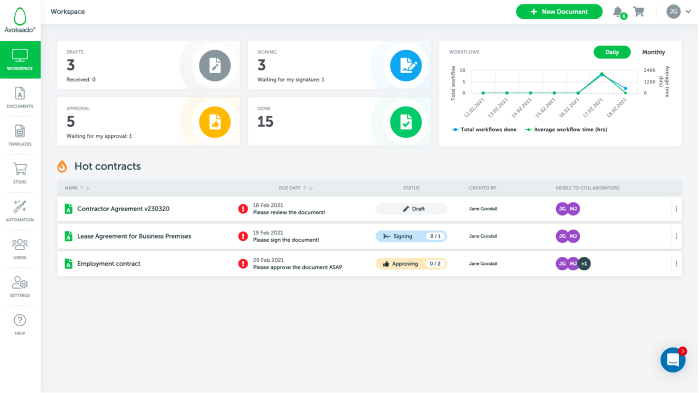
\includegraphics[width=13cm]{./assets/avokkado.png}
  \caption{รูปแสดงซอฟแวร์ของ Avokkado}\label{fig:avokkado}
\end{figure}

\newpage
\subsection{ContractSafe application}
\hspace*{1cm} ContractSafe \cite{BestDMS,WhatIsContractSafe} เป็น Document management system ที่มีจุดเด่นในเรื่องของการใช้ AI เป็นตัวช่วยในการค้นหาและสแกนเอกสาร ทำให้สามารถค้นหาและแสกนเอกสารได้อย่างรวดเร็ว อีกทั้งยังมีระบบรักษาความปลอดภัยของข้อมูลเอกสาร โดยผ่านมาตรฐานการรับรองของ SOC2 \\
\hspace*{1cm} ข้อดีของ ContractSafe มีดังนี้
\begin{itemize}
  \item มีการจัดการจัดเก็บที่ปลอดภัย และสามารถแสกนได้อย่างรวดเร็ว	
  \item สามารถจัดการกับสิทธิการเข้าถึงข้อมูลได้แลมีการติดตามที่ชัดเจน
  \item มีระบบการแจ้งเตือนทางอีกเมล และมีการเขียนรายงานที่อ่านง่ายไม่ซับซ้อน
\end{itemize}

\begin{figure}[!h]\centering
  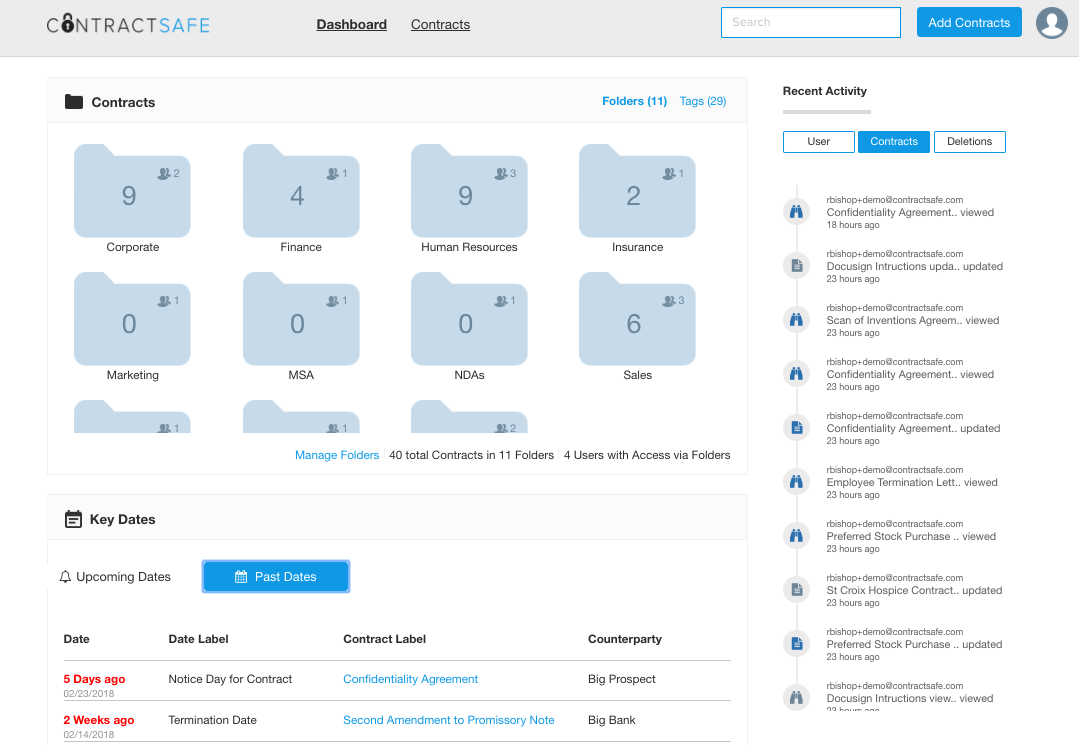
\includegraphics[width=13cm]{./assets/contractsafe.png}
  \caption{รูปแสดงซอฟแวร์ของ Contractsafe}\label{fig:contractsafe}
\end{figure}


\subsection{Laserfiche application}
\hspace*{1cm} Laserfiche \cite{WhatIsLaserFiche} สามารถปรับแต่งซอฟแวร์หรือกำหนดรูปแบบของซอฟแวร์ได้อย่างอิสระ เพื่อให้สอดคล้องกับความต้องการของแต่ละบริษัท ทำให้ลดข้อผิดพลาดที่อาจจะเกิดขึ้น และสามารถดำเนินการได้อย่างครบถ้วน ซึ่งจุดเด่นของ Laserfiche นั้นจะเป็นในรูปแบบของ Config Flow ก็คือรูปแบบการทำงานที่จะสามารถย้อนกลับมาแก้ไขไฟล์ได้ตลอดเวลา ซึ่งถ้าหากเจอข้อผิดพลาดก็ไม่ต้องยกเลิก หรือต้องเสียเวลาเริ่มต้นกระบวนการใหม่ทั้งหมด \\
\hspace*{1cm} โดยจุดเด่นของ Laserfiche จะมีดังนี้
\begin{itemize}
  \item ค้นหาเอกสารได้อย่างรวดเร็ว
  \item ค้นหาข้อมูลด้วย Text จากเอกสารสแกน
  \item จัดระเบียบข้อมูลและเอกสารได้ตามต้องการ
  \item สามารถย้อนกลับมาแก้ไขไฟล์ได้ตลอดเวลา
\end{itemize}

\begin{figure}[!h]\centering
  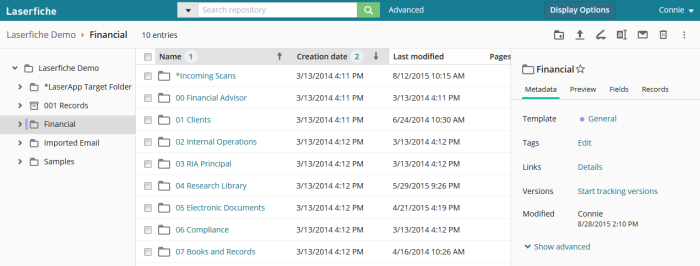
\includegraphics[width=13cm]{./assets/laserfiche.png}
  \caption{รูปแสดงซอฟแวร์ของ Laserfiche}\label{fig:laserfiche}
\end{figure}

\subsection{Amagno application}
\hspace*{1cm} Amagno \cite{WhatIsAmagno} คือเครื่องมือสำคัญสำหรับองค์กรเพื่อเอาไว้ใช้บริหารจัดการคอนเทนท์ต่าง ๆ ที่มีอยู่มากมายและกระจัดกระจาย ให้กลับมาเป็นระเบียบเรียบร้อย โดยจะสามารถตรวจสอบและค้นหาเอกสารได้อย่างรวดเร็ว อีกทั้งยังสามารถกำหนดสิทธิการเข้าถึงเพื่อเพิ่มความปลอดภัยให้กับข้อมูลที่สำคัญขององค์กร \\
\hspace*{1cm} โดยจุดเด่นของ Amagno มีดังนี้
\begin{itemize}
  \item ป้องกันเอกสารไม่ให้ถูกลบหรือแก้ไขซ้ำ
  \item ป้องกันเอกสารซ้ำด้วยการเปรียบเทียบเวอร์ชั่นเอกสารล่าสุด
  \item สแกนเอกสารกระดาษเข้าระบบได้โดยตรง
  \item รองรับไฟล์ข้อมูลเอกสารได้ทุกรูปแบบ
\end{itemize}
\begin{figure}[!h]\centering
  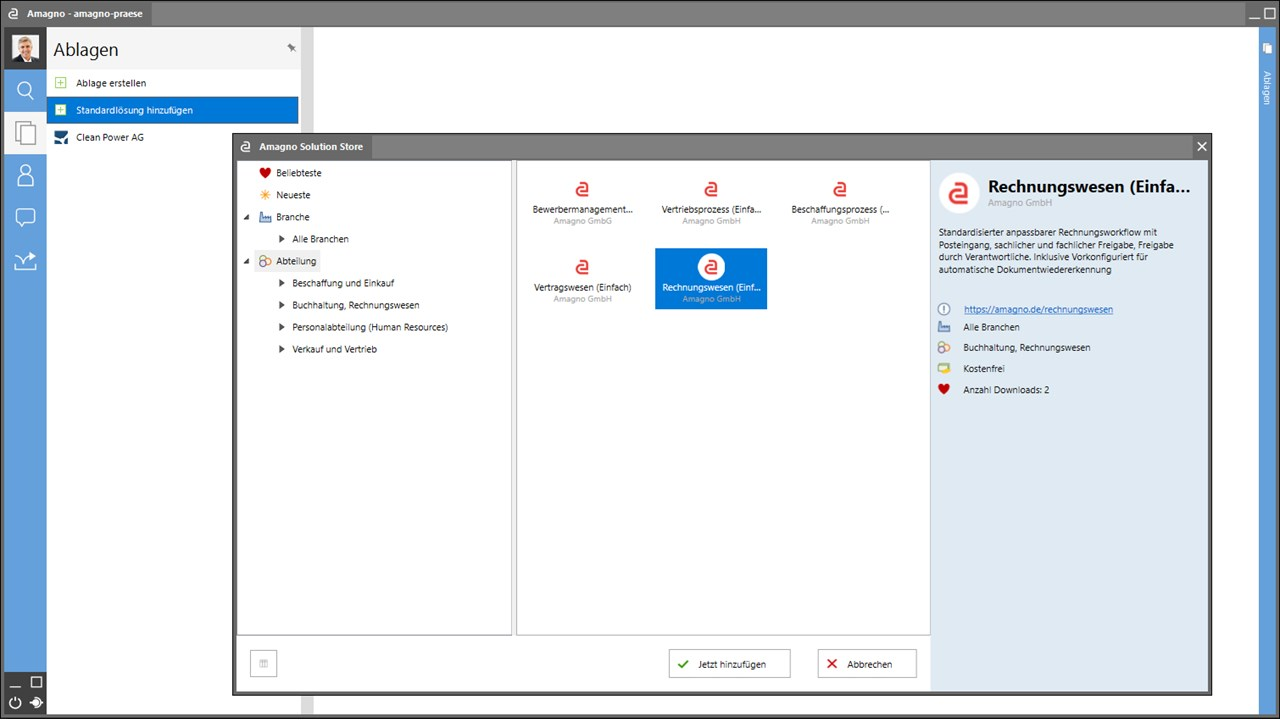
\includegraphics[width=13cm]{./assets/amagno.png}
  \caption{รูปแสดงซอฟแวร์ของ Amagno}\label{fig:amagno}
\end{figure}

\clearpage
\section{เปรียบเทียบผลิตภัณฑ์ที่เกี่ยวข้อง}
\hspace{1cm} การเปรียบเทียบผลิตภัณฑ์ที่มีความคล้ายคลึงและมีความเกี่ยวข้องกับระบบที่ทางคณะผู้จัดทำทำขึ้นในปริญญานิพนธ์นี้แสดงได้ดังตารางที่ \ref{tbl:productsTable} ดังนี้
\begin{table}[!ht]
    \begin{tabular}{|c|c|c|c|c|c|}
    \hline
                                           & D-LAW & Avokaado & ContractSafe & Laserfiche & Amagno \\ \hline
    ระบบค้นหา เอกสาร                       & \checkmark     & \checkmark        & \checkmark            & \checkmark          & \checkmark      \\ \hline
    ระบบจัดการสิทธิการเข้าถึงข้อมูล เอกสาร & \checkmark     &          & \checkmark            &            & \checkmark      \\ \hline
    ระบบเผยแพร่เอกสาร                      & \checkmark     &          & \checkmark            &            &        \\ \hline
    ระบบร่างเอกสาร                         & \checkmark     & \checkmark        &              &            &        \\ \hline
    ระบบสร้างกำหนดการ                      & \checkmark     &          &              &            &        \\ \hline
    รองรับ ภาษาไทย                         & \checkmark     &          &              & \checkmark          & \checkmark      \\ \hline
    \end{tabular}
    \caption{\centering  ตารางเปรียบเทียบผลิตภัณฑ์ใกล้เคียงกับ D-LAW} \label{tbl:productsTable}
\end{table}

\section{เทคนิคและเทคโนโลยีที่ใช้}
\subsection{Frontend framework}
\begin{itemize}
  \item \textbf{NextJS} \\
\hspace*{1cm} เป็น Framework ที่ใช้สำหรับเขียนเว็บ โดยพัฒนามาจาก React ซึ่ง ออกแบบมาให้ใช้งานง่ายมี learning curve ต่ำ โดยตัว NextJS มีคามโดดเด่นด้านการทำ SSR (Server-side-rendering) และยังมีการทำ Routing ที่เข้าใจได้ง่ายมี Folder structure ที่ชัดเจน  \\
\hspace*{1cm} เนื่องจาก NextJS มี learning curve ที่ต่ำ และไม่จำเป็นต้อง optimize มากนัก เนื่องจากตัว Framework ได้ทำการ optimize มาในบางส่วนแล้ว เลยทำให้สามารถเริ่ม ทำงานได้เลย และอยู่ในมาตรฐานของเว็บไซต์ทั่วไป \cite{WhaiIsNextJS}
  \item \textbf{Antd} \\
\hspace*{1cm} คือ React UI library ที่มี  Component ให้ใช้ที่ค่อนข้างครอบคลุม หลากหาย และสวยงาม ซึ่งสามารถรองรับ Responsive ได้เป็นอย่างดี \\
\hspace*{1cm} ดังนั้น เราจึงเลือกใช้ antd เพื่อที่จะมาลดเวลา การทำ Base component ต่าง ๆ ซึ่งคิดว่าในส่วนของการทำเว็บ ตัว Base component นั้นใช้เวลาในการ พัฒนามากที่สุด และ antd ยังสามารถ กำหนด Rule ต่าง ๆ เพื่อ handling error ต่าง ๆ ได้สะดวกขึ้น \cite{WhaiIsAntd}
  \item \textbf{Tailwind} \\
\hspace*{1cm} คือ Utility-First CSS Framework สำหรับจัดการ HTML Element โดยตรง ซึ่ง Tailwind ออกแบบมาให้เป็น low-level class ทำให้ตัวไฟล์มีขนาดที่เล็กมาก และจากที่ Tailwind มี class ให้ใช้ค่อนข้างครอบคลุม และการทำ Custom class element ได้ง่ายขึ้น และที่สำคัญ Tailwind เป็น CSS Framework ที่ทำ responsive ค่อนข้างง่าย \\
\hspace*{1cm} ดังนั้น การนำ Tailwind มาใช้ในการทำเว็บไซต์จะนำมาช่วยทำ layout ต่าง ๆ ในเว็บ และทำในส่วนของ custom class element ให้ง่าย และเร็วมากขึ้น \cite{WhaiIsTailwind}
\end{itemize}
\subsection{Backend framework}
\begin{itemize}
  \item \textbf{Go language} \\
  \hspace*{1cm} เป็นภาษาที่มีความเร็วสูง และมีความปลอดภัยสูง ซึ่งเป็นภาษาที่เหมาะสำหรับการทำ API อีกทั้งยังมีจุดเด่นในด้านของความง่ายในการอ่านและเขียน ที่สำคัญยังสามารถเขียนโค้ดให้เป็นในรูปแบบของ Concurrent Programming ได้ง่าย \cite{WhatIsGo, WhatIsConcurrentProgramming}
  \item \textbf{Gin framework} \\
\hspace*{1cm} เป็น web Framework ที่เขียนด้วยภาษา Golang ซึ่งมีประสิทธิภาพด้านความเร็วที่สูงมาก และเป็นที่นิยมในกลุ่มนักพัฒนา โดย Gin นั้นยังสามารถพัฒนาออกมาให้เป็นในรูปแบบของไมโคเซอวิสได้ อีกทั้งยังสามารถจัดการกับ error ที่เกิดขึ้นในระหว่าง HTTP request ได้อย่างง่ายดายโดย Gin  จะมีการเก็บรวมรวม error ไว้ซึ่งจะทำให้สามารถใช้ Middleware จัดการ error ต่อได้ง่าย \cite{WhatIsGin}
\end{itemize}
\subsection{Database}
\begin{itemize}
  \item \textbf{PostgreSQL} \\
\hspace*{1cm} เป็น RDBMS ที่ใช้งานอย่างแพร่หลาย และมีความสามารถหลากหลาย เช่น สามารถเก็บ Data type เป็น Array หรือ JSON ได้ และสามารถใช้งานได้ในรูปแบบของ Multi-Version Concurrency Control หรือ MVCC ทำให้สามารถใช้ PostgreSQL ในเวอร์ชันที่แตกต่างกันได้ เป็นต้น อีกทั้งยังเป็น Open source ทำให้สามารถนำไปแก้ไขหรือนำไปใช้งานได้ฟรี \cite{WhatIsPostgresQL}
  \item \textbf{Elasticsearch} \\
\hspace*{1cm} Elasticsearch \cite{WhatIsElasticsearch, ElasticsearchForSearchEngine} เป็น database ซึ่งเปิดตัวในปี 2010 โดยบริษัท Elasticsearch N.V. ที่มีเครื่องมือค้นหาและการวิเคราะห์ที่ถูกสร้างขึ้นบน Apache Lucene ซึ่งถูกพัฒนาด้วยภาษา Java โดย Elasticsearch สามารถเก็บข้อมูลได้หลายประเภททั้งข้อความ ตัวเลข structured data และ unstructured data และสิ่งที่ทำให้เป็นจุดเด่นคือเรื่องของความเร็วในการจัดเก็บ ค้นหา และวิเคราะห์ข้อมูลในปริมาณมาก ๆ ได้ ซึ่งเป็นความเร็วในหน่วยมิลลิวินาที เนื่องจาก Elasticsearch มีการเก็บข้อมูลอยู่ในรูปแบบ JSON และทาง Elasticsearch จะทำการแปลงเป็น index และจัดเก็บไว้ ถ้าให้เปรียบเทียบก็คือการนำข้อมูลมาจัดเรียงให้มีลักษณะคล้ายกับสารบัญ เมื่อทำการค้นหาจะทำให้ค้นหาได้ไว อีกทั้ง Elasticsearch ยังมีระบบ relevancy เป็นการทำให้ระบบรู้ว่าควรจะแสดงผลลัพธ์อะไรให้ตรงกับที่ต้องการมากที่สุดซึ่งมีการใช้วิธีการประเมินที่เรียกว่า Term Frequency-Inverse Document Frequency (TF-IDF) ก็คือ ยิ่งข้อความหรือคำที่หานั้นตรงมีอยู่ในเอกสารเยอะขนาดไหน ก็แสดงว่าเอกสารหรือข้อมูลชุดนั้นก็มีความเกี่ยวข้องมากและยิ่งจำนวนเอกสารที่มีในการค้นหามากเท่าไหร่แสดงว่า คำหรือข้อความที่ค้นหานั้นมีความสำคัญน้อยลง ซึ่งการใช้วิธีการประเมินนี้ทำให้ได้ผลลัพธ์ที่ออกมาได้รวดเร็ว ซึ่งสามารถใช้งานได้โดยการใช้ Elasticsearch API ในการค้นหาได้ แต่ Elasticsearch ไม่ใช่เป็นเพียงแต่ database ที่มีเอาไว้ใช้ในการเก็บข้อมูลและใช้ในการค้นหาเท่านั้น แต่ว่ายังมีระบบแสดงผลที่เรียกว่า Kibana ซึ่งจะแสดงผลให้เห็นข้อมูลต่าง ๆ ให้อยู่ในรูปแบบแผนภูมิ แผนที่ และฟิลเตอร์ได้
\end{itemize}
\subsection{Version control}
\begin{itemize}
  \item \textbf{Github} \\
\hspace*{1cm} เป็น Version control ซึ่งข้อดีของมันก็คือการเก็บข้อมูลไว้เป็นเวอร์ชันได้ ซึ่งเหมาะกับการทำงานกันเป็นทีม โดยไม่ว่าจะเป็นการแก้ไข ตรงไหนสมาชิกในทีมก็จะรู้ได้ทั้งหมด ซึ่ง github สามารถใช้งานในรูปแบบของ free plan ได้ \cite{WhatIsGithub}
\end{itemize} 

\subsection{Cloud}
\begin{itemize}
\item \textbf{Google cloud storage} \\
\hspace*{1cm} คือ บริการ Storage ของ Google cloud ที่ให้บริการฝากรูป, ไฟล์ ต่าง ๆ ประเภทข้อมูลที่เป็น Unstructure data ขนาดใหญ่ มีการเปิด API ในการจัดการไฟล์ต่าง ๆ ทำให้สามารถเขียนโปรแกรมเพื่ออัพโหลด หรือดาวโหลดไฟล์เพื่อนำมาใช้งานได้ \\
\hspace*{1cm} เนื่องจาก คณะผู้จัดทำมีการเก็บไฟล์ประเภทรูปและเอกสารต่าง ๆ เช่น รูปโปรไฟล์ผู้ใช้งาน เอกสารของทนาย จึงเลือกใช้ Google cloud storage ในเก็บข้อมูลเพื่อที่จะได้ไม่ต้องจัดการกับการจัดเก็บไฟล์ อีกทั้งในอนาคตยังสามารถ scale ได้ง่ายเพราะว่าไฟล์มีการ จัดเก็บอยู่บน Cloud ไม่ใช่เครื่องใดเครื่องหนึ่ง \cite{WhatIsGoogleStorage}
\item \textbf{Google cloud Virtual Machine} \\
\hspace*{1cm} คือ บริการ Virtual Machine ของ Google cloud เพื่อใช้ในการ deploy ทั้งหลังบ้านและ database และอีกเหตุผลที่ใช้ vm ของ google เพราะ google cloud มี service ต่าง ๆ อีกมากมายที่สามารถใช้งานได้ \cite{WhatIsVM,WhatIsGoogleCloudPlatform}
\item \textbf{Google calendar API} \\
\hspace*{1cm} คือ บริการ RESTful API ของ Google โดยจะให้บริการในรูปแบบปฏิทินและกรรม ทำให้สามารถทำการเชิญให้ผู้อื่นสามารถใช้หรือแชร์ปฏิทินร่วมกับผู้อื่นได้ โดยผู้ได้รับเชิญสามารถยอมรับหรือปฏิเสธคําเชิญได้ \cite{WhatIsGoogleCalendar}
\item \textbf{Google Vision} \\
\hspace*{1cm} Google vision  คือ บริการ Cloud Vision API ของ Google cloud โดยจะเป็น AI-ML ที่จะช่วยวิเคราะห์หรือสแกน รูปภาพสินค้า หรือเอกสารต่าง ๆ ให้ออกมาในรูปแบบตาม Model ที่เลือกใช้ \cite{WhatIsGoogleVision}
\end{itemize}

\subsection{Planning \& Discuss tools}
\begin{itemize}
\item \textbf{Trello} \\
\hspace*{1cm} Trello เป็นแอปพลิเคชันที่ใช้เพื่อจัดการวางแผนงานหรือขั้นตอนการทำงาน โดยจะทำเป็นลักษณะของ Kanban board ซึ่งสามารถติดตามสถานะต่าง ๆ และปริมาณงานได้ \cite{WhatIsTrello}
\item \textbf{Figma and FigJam} \\
\hspace*{1cm} Figma เป็นแอปพลิเคชันที่มีความสามารถในการออกแบบ flow และ UI ของเว็บแอปพลิเคชันอีกทั้ง ยังสามารถใช้งานได้ง่ายผ่าน Web browser ได้โดยตรง ซึ่ง FigJam เป็นอีกฟังก์ชันหนึ่งในตัว Figma ที่มีลักษณะเป็นไวท์บอร์ดสามารถที่จะเขียนข้อความต่าง ๆ ได้ โดยเหมาะที่จะมาใช้ในการระดมความคิด \cite{WhatIsFigma}
\item \textbf{Discord} \\
\hspace*{1cm} Discord เป็นแอปพลิเคชันที่ใช้สำหรับการสื่อสารที่สามารถสื่อสารได้ทั้งเสียงและข้อความโดยสามารถแบ่งแยกห้องออกมาเป็นหมวดหมู่ได้ \cite{WhatIsDiscord}
\end{itemize}

\hspace*{1cm}  จากการศึกษาข้อมูลของกาวิธีการดำเนินคดีของทนายความจะนำไปใช้ในการระบุหมวดหมู่ที่ใช้ในระบบและมีการใช้ RESTful API เป็นช่องทางในการติดต่อระหว่างส่วน Front-end และส่วน Back-end ซึ่งในระบบของเราก็จะมีการทำ Data visualization เพื่อให้บุคคลทั่วไปสามารถเข้ามาและสามารศึกษาข้อมูลได้ และอีกหนึ่งส่วนที่ใช้คือ OCR ซึ่งเป็นส่วนที่ใช้ในการแปลงรูปภาพของเราให้กลายเป็นข้อความเพื่อที่จะสามารถใช้ในการจัดการข้อมูลของระบบเราได้ และท้ายสุดเราเลือกใช้เทคโนโลยีต่าง ๆ ให้เหมาะสมกับระบบของเราประกอบกับความสนใจของผู้พัฒนา\\

% \hspace*{1} ซึ่งในปัจจุบันทนายนั้นทีเครื่องมือที่ใช้อยู่คือ Google drive เพื่อใช้จัดเก็บเอกสารและ File explorer ที่อยู่ในเครื่องคอมพิวเตอร์ window และทนายบางรายมีการใช้ Google calendar เพื่อใช้ในการบันทึกข้อมูลของแต่ละคนและจะมี notion เพื่อใช้ในการให้ลูกความได้ดูข้อมูลและนัดหมาย ซึ่งระบบของเรานั้นจะมีการใช้งานเบื้องต้นจะเหมือนกับการจัดไฟล์ให้เป็นระบบ อีกทั้งยังมีการทำเพิ่มความ 

%%%%%%%%%%%%%%%%%%%%%%%%%%%%%%%%%%%%%%%%%%%%%%%%%%%%%%%%%%%%
%%%%%%%%%%%%%%%%%%%%%%% CHAPTER3 %%%%%%%%%%%%%%%%%%%%%%%%%%%
%%%%%%%%%%%%%%%%%%%%%%%%%%%%%%%%%%%%%%%%%%%%%%%%%%%%%%%%%%%%
\chapter{วิธีการดำเนินงาน กระบวนการและการออกแบบ}

ในส่วนบทที่ 3 จะกล่าวถึงรายโครงสร้างของระบบหรือรูปแบบการออกแบบต่าง ๆ อาทิเช่น UML diagram, Usecase diagram เป็นต้น

\section{สถาปัตยกรรมระบบ}
\hspace*{1cm} เว็บแอปพลิเคชัน Document management system for lawyer สามารถแบ่งการทำงานได้เป็น 5 ส่วนย่อยแสดงดังรูป \ref{fig:systemArch} โดยมีสถาปัตยกรรม ดังนี้
\begin{enumerate}
  \item \textbf{Front-end} \\
  \hspace*{1cm} เป็นส่วนที่ใช้แสดง User interface เพื่อติดต่อกับ User โดยทำการต่อกับ Back-end โดยใช้ API โดยในส่วนนี้จะประกอบไปด้วย
  \begin{itemize}
    \item Document management system: สำหรับจัดการเคสและเอกสาร
    \item Appointment system: สำหรับส่งนัดหมายไปสู่ทนายและลูกความ
    \item Tracking system: สำหรับติดตามสถานะและวันนัดหมายของคดี
  \end{itemize}
  \item \textbf{Back-end} \\
  \hspace*{1cm} เป็นส่วนที่ใช้ในการประมวลผล และจัดการข้อมูลต่าง ๆ ซึ่งทำการเชื่อมต่อกับ Database และ Service ต่าง ๆ คือ OCR , Storage , Google calendar API เพื่อใช้ในการประมวลผลก่อนที่จะนำไปแสดงผลต่อในส่วนของ Front-end 
  \item \textbf{Database} \\
  \hspace*{1cm} เป็นส่วนที่ใช้ในการเก็บข้อมูลต่าง ๆ ของเว็บแอปพลิเคชัน เช่น ข้อมูลผู้ใช้ ข้อมูลไฟล์ ข้อมูลคดี ต่าง ๆ เป็นต้น โดยมีการใช้ Database อยู่ 2 ชนิด ก็คือ PostgreSQL และ ElasticSearch 
  \item \textbf{OCR} \\
  \hspace*{1cm} เป็นส่วนที่ใช้ในการจัดการแปลงไฟล์เอกสารหรือไฟล์รูปภาพให้อยู่ในรูปแบบข้อความเพื่อที่จะใช้ในการเก็บข้อมูลเข้า Database เพื่อใช้ในการค้นหา
  \item \textbf{Storage} \\
  \hspace*{1cm} เป็นส่วนที่ใช้ในการจัดเก็บไฟล์ต่าง ๆ ไม่ว่าจะเป็นไฟล์รูปภาพ หรือไฟล์เอกสารต่าง ๆ 
  \item \textbf{Google calendar API} \\
  \hspace*{1cm} เป็น Service ที่ใช้ในการสร้างและแก้ไขนัดหมายต่าง ๆ
\end{enumerate}

\begin{figure}[!ht]\centering
  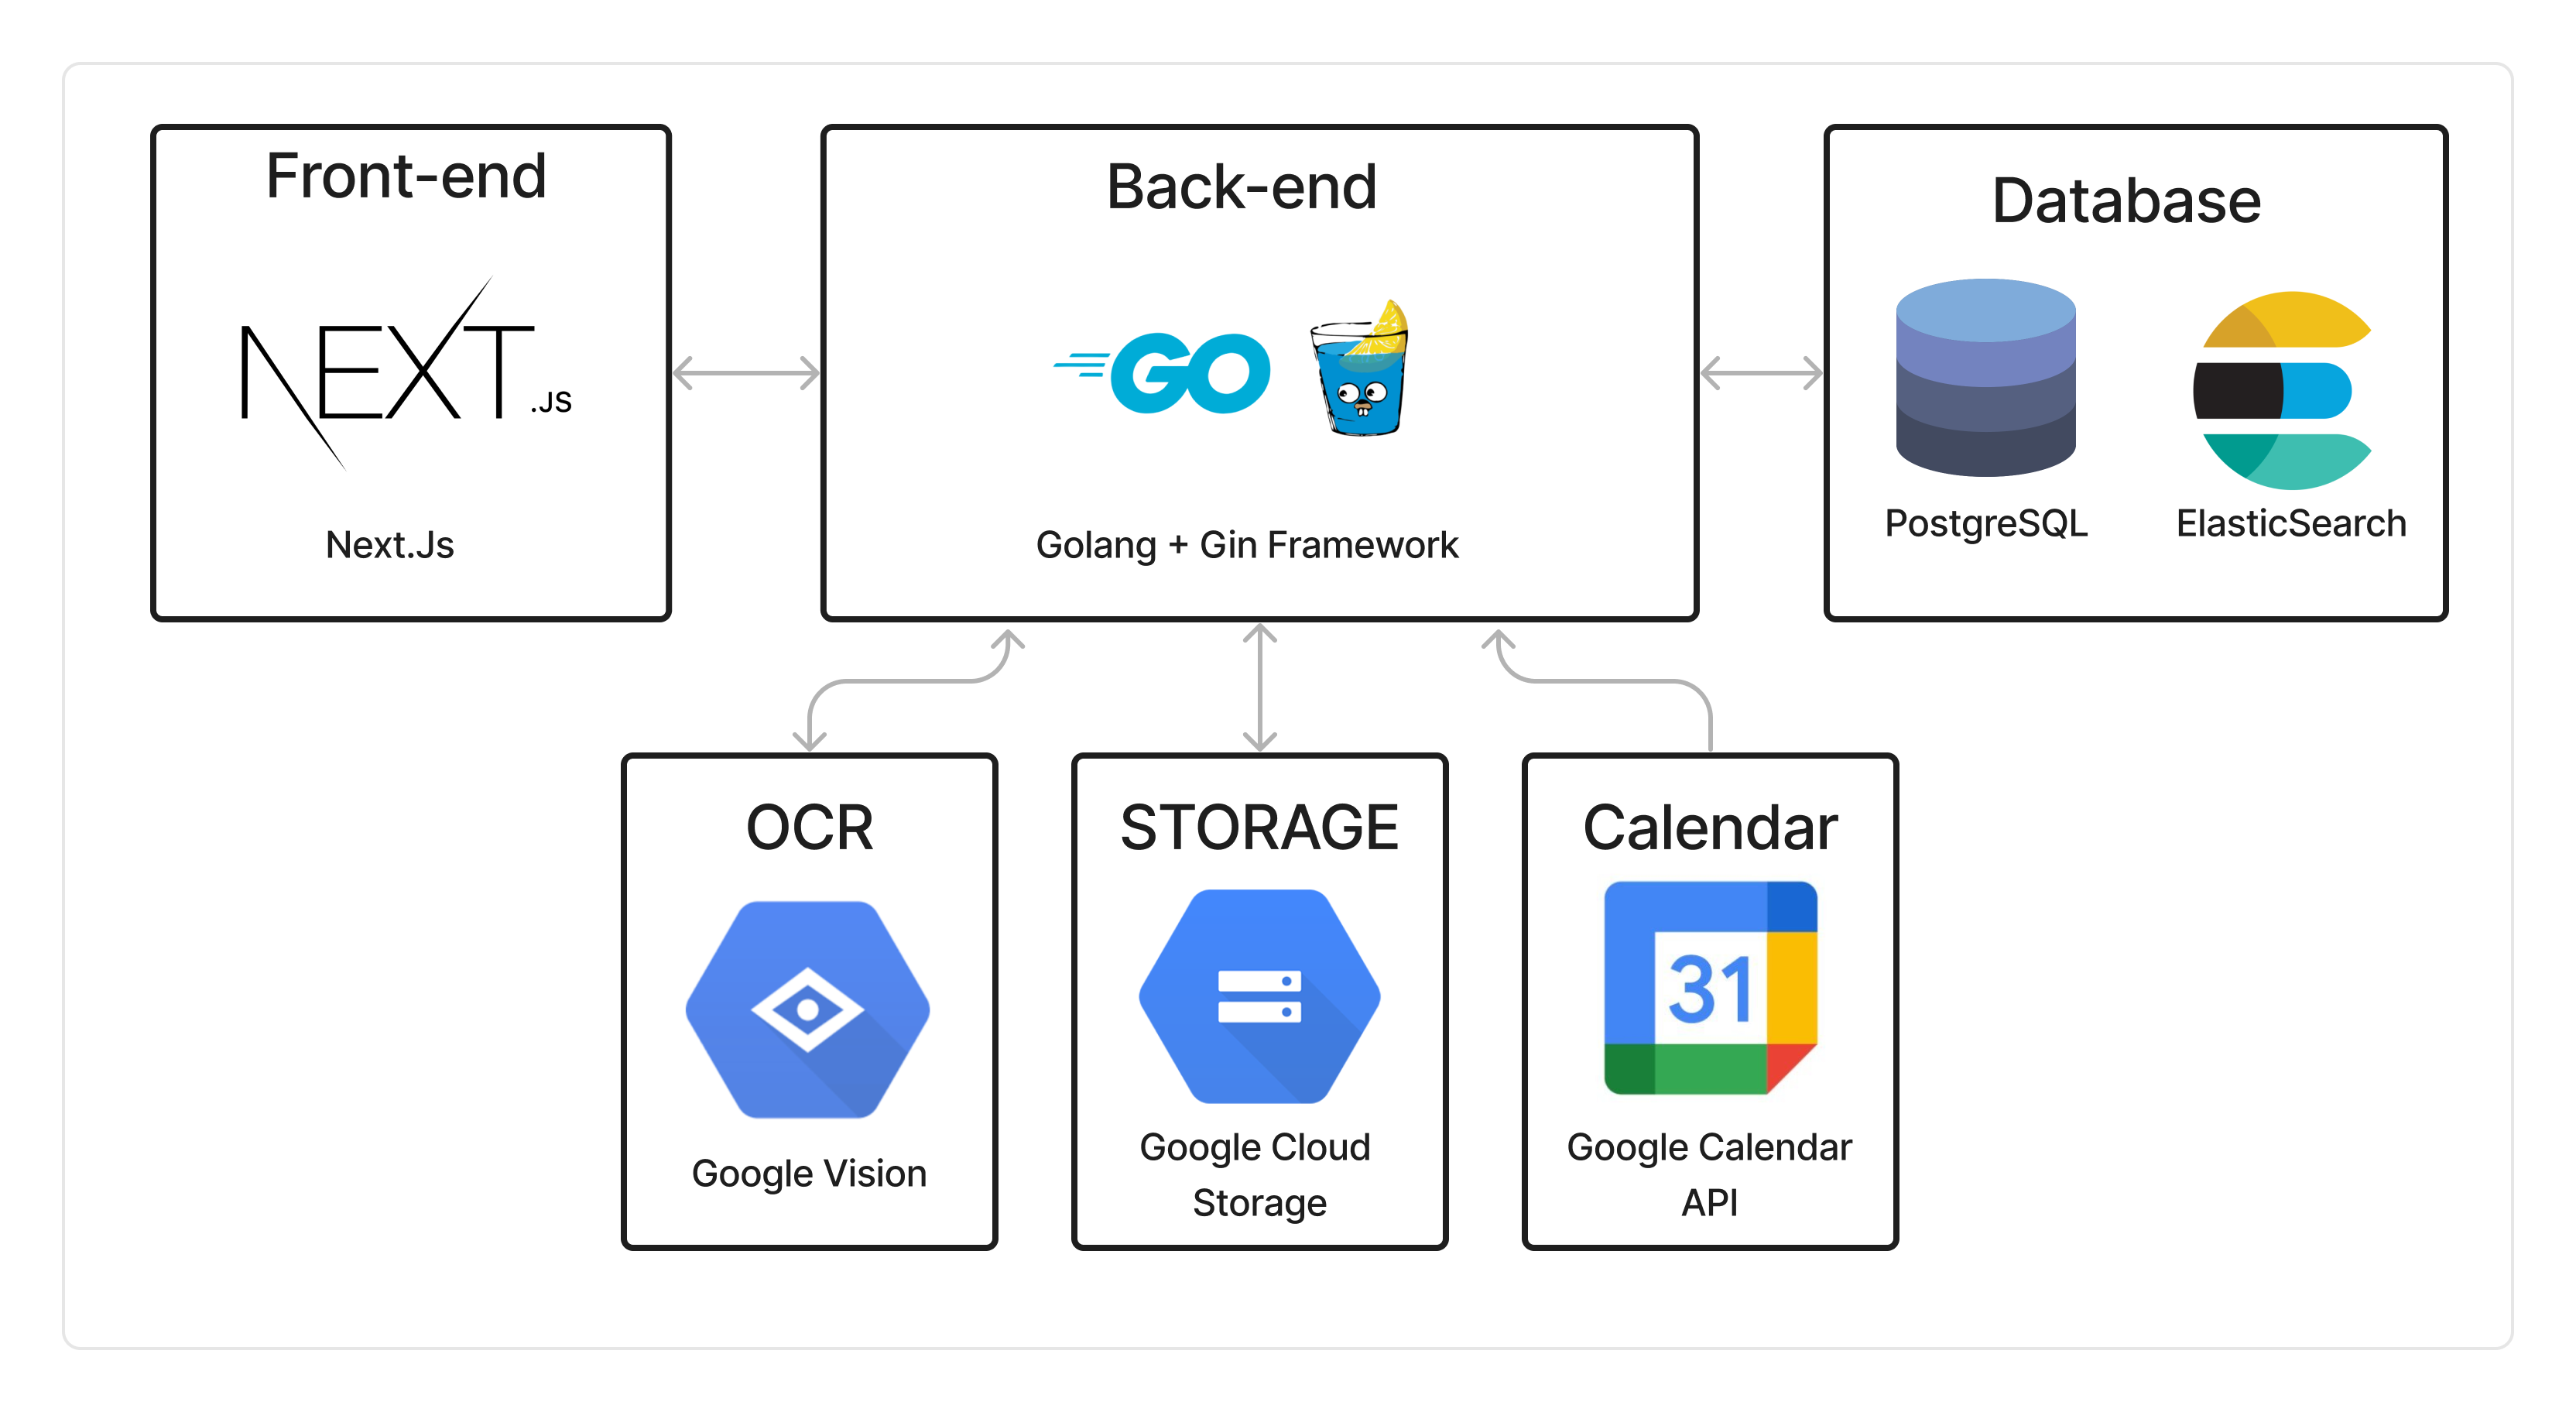
\includegraphics[width=13cm]{./assets/system-arch.png}
  \caption{รูปแสดงสถาปัตยกรรมระบบของซอฟแวร์}\label{fig:systemArch}
\end{figure}

\newpage

\section{ข้อกำหนดและความต้องการของระบบ}
\begin{enumerate}
  \item สามารถแสดงเคสโฟล์เดอร์ และไฟล์เอกสารต่าง ๆ รวมไปถึงสามารถสร้าง อัพโหลด ลบ เผยแพร่ รวมไปถึงจัดการสิทธการเข้าถึง เคสโฟล์เดอร์ได้
  \item สามารถค้นหาเอกสารผ่านคำค้นหา แท๊ก หรือชนิดของไฟล์เอกสารได้
  \item สามารถเข้าไปดูรายระเอียดเนื้อหาของไฟล์เอกสารได้
  \item สามารถกำหนดนัดหมาย และส่งนัดหมายไปยัง google calendar และ email ได้
  \item สามารถแก้ไขข้อมูลส่วนตัว รวมไปถึงเพิ่มหรือแก้ไขผู้ใช้งานในระบบได้
  \item สามารถค้นหาคดีต่าง ๆ โดยใชหมายเลขคดีดำ หรือหมายเลขคดีแดงได้ โดยจะแสดงรายละเอียดต่าง ๆ ของคดีที่ทำการค้นหา
  \item สามารถแสดงข้อมูลในรูปแบบของแผนภูมิรูปแบบต่าง ๆ ที่เกี่ยวข้องกับกฎหมาย หรือคดีต่าง ๆ
\end{enumerate}

\clearpage
\section{Navigation map}
\hspace*{1cm}โดย Navigation map จะแบ่งออกเป็น 2 ส่วน คือ ส่วนของผู้ใช้งานทั่วไปแสดงดังรูปที่ \ref{fig:navMapGuest} และส่วนของผู้ใช้งานที่เป็นทนายแสดงดังรูปที่ \ref{fig:navMapLawyer} \\

\hspace{1cm}โดยในส่วนของผู้ใช้งานทั่วไปเมื่อเข้าใช้งานเว็บแอปพลิเคชันจะเริ่มต้นที่หน้า Landing ซึ่งในหน้านี้มีจะมีการแสดงแผนที่จำลองหรือในรูปแบบแผนภูมิซึ่งจะสามารถไปยังหน้าอื่น ๆ ได้ 2 หน้า โดยมีหน้าแรกคือ 
หน้า Case search ซึ่งเป็นหน้าที่ใช้ในการติดตามโดยค้นหาจากเลขคดี และหน้า Appointment list จะเป็นหน้าที่สามารถดูนัดหมายที่ได้รับการเผยแพร่ได้  \\
\begin{figure}[!ht]\centering
    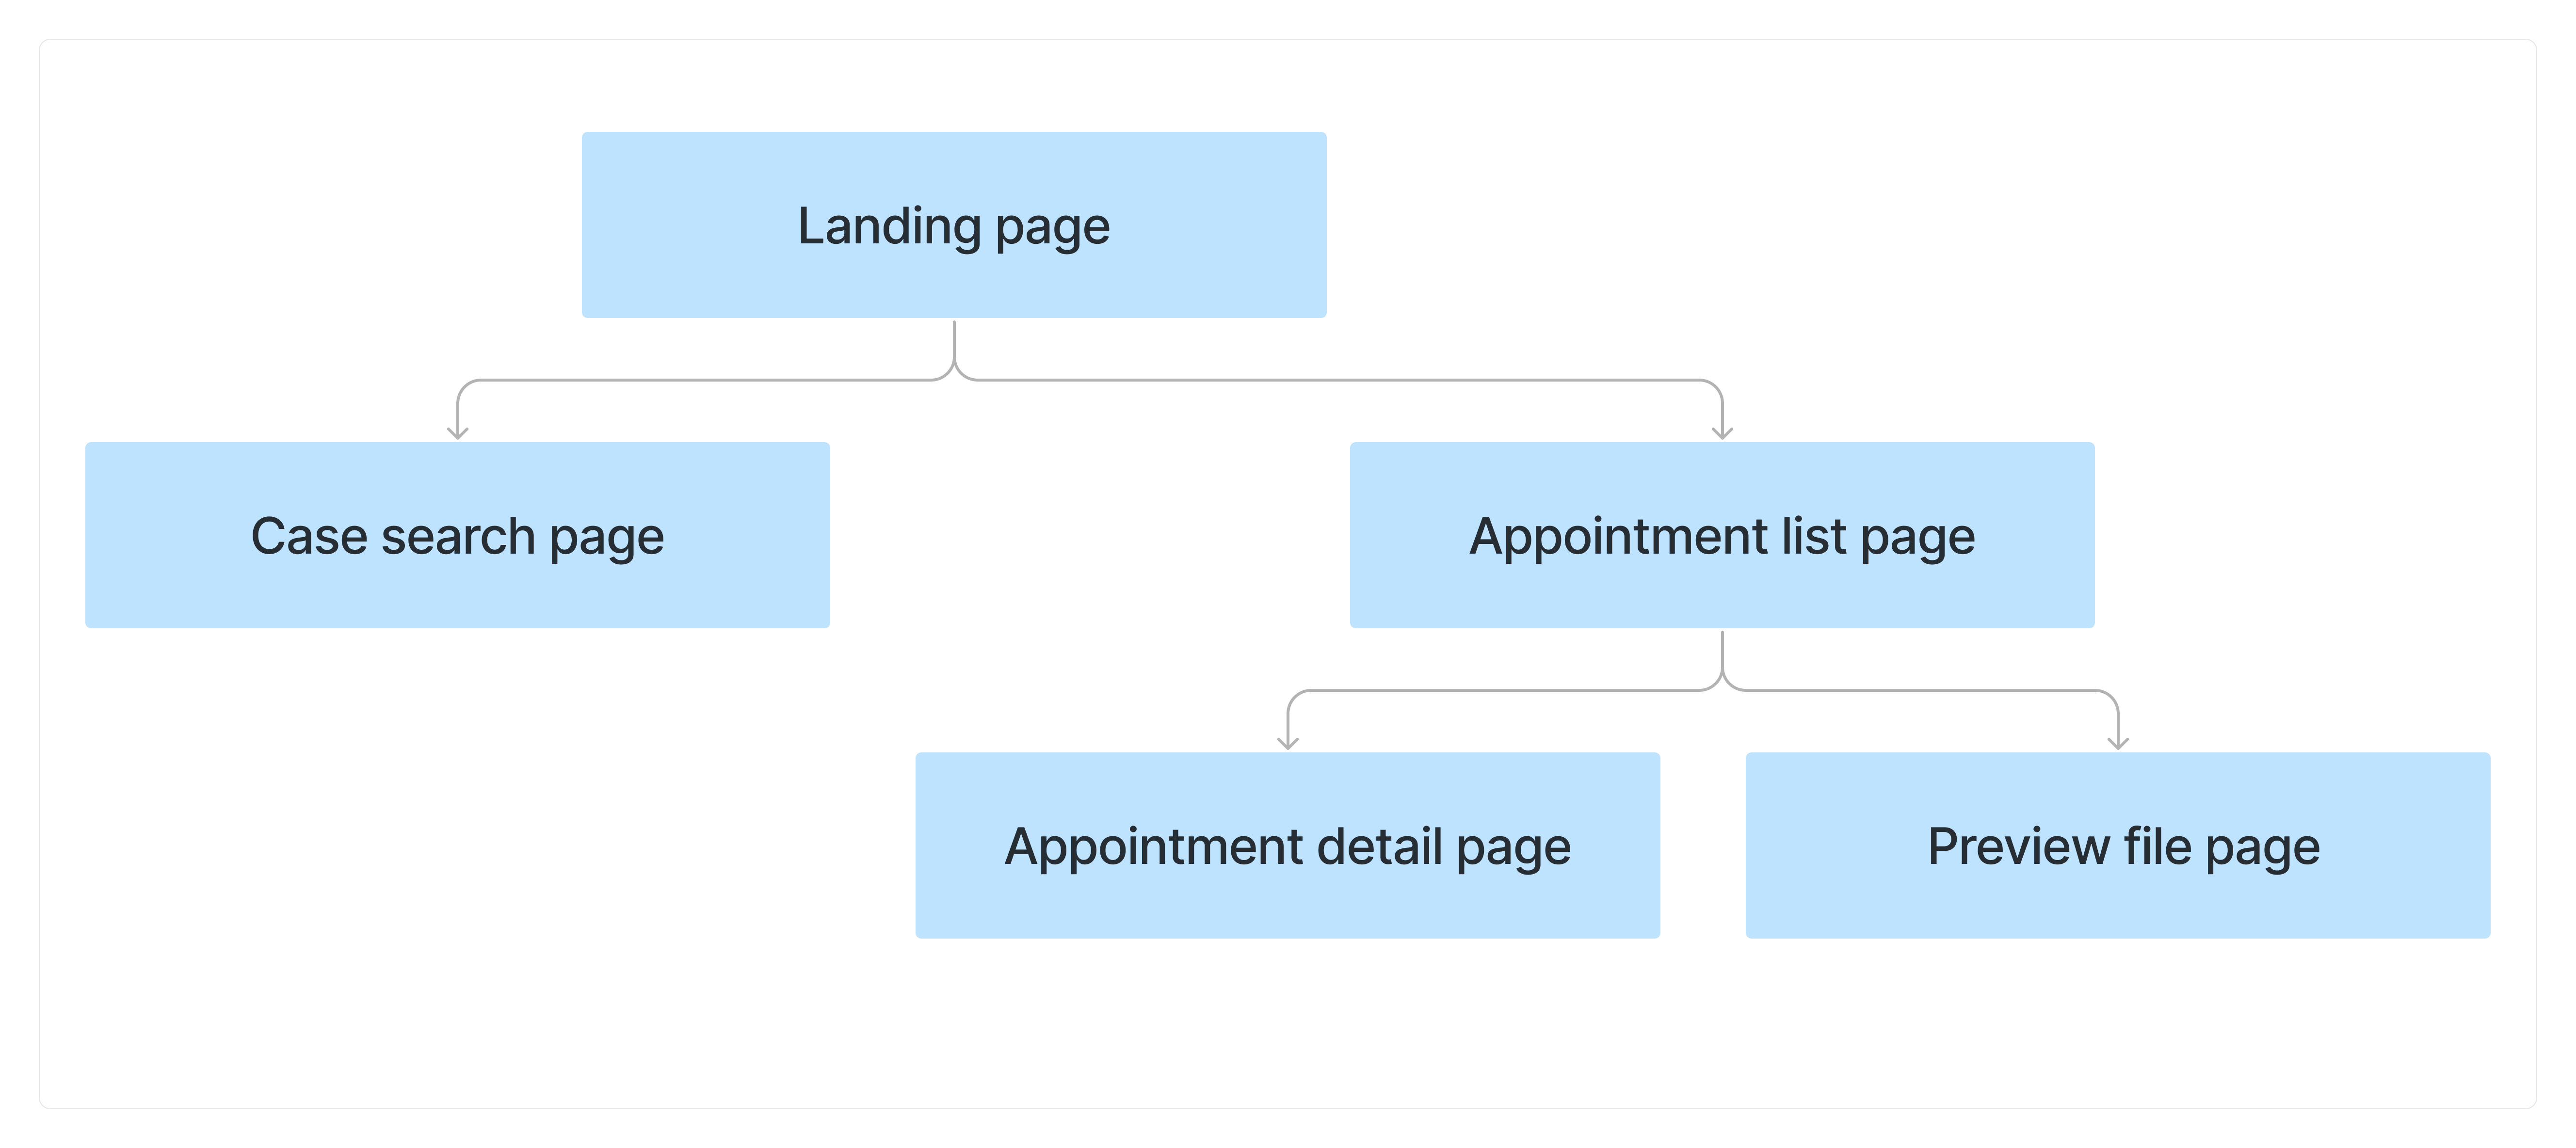
\includegraphics[width=13cm]{./assets/nav-map-guest.png}
    \caption{รูปแสดง Navigation map ของบุคคลทั่วไป}\label{fig:navMapGuest}

\end{figure}

\hspace{1cm}ในส่วนของทนายความจะเริ่มต้นที่หน้า Landing จากนั้นเข้ามาหน้า Login เมื่อเข้าสู่ระบบสำเร็จจะเข้ามาที่หน้า Home ซึ่งสามารถติดตามคดีต่าง ๆ จัดการเอกสาร รวมไปถึงการดูนัดหมายและตั้งค่าข้อมูลส่วนตัวได้ \\
\begin{figure}[!ht]\centering
    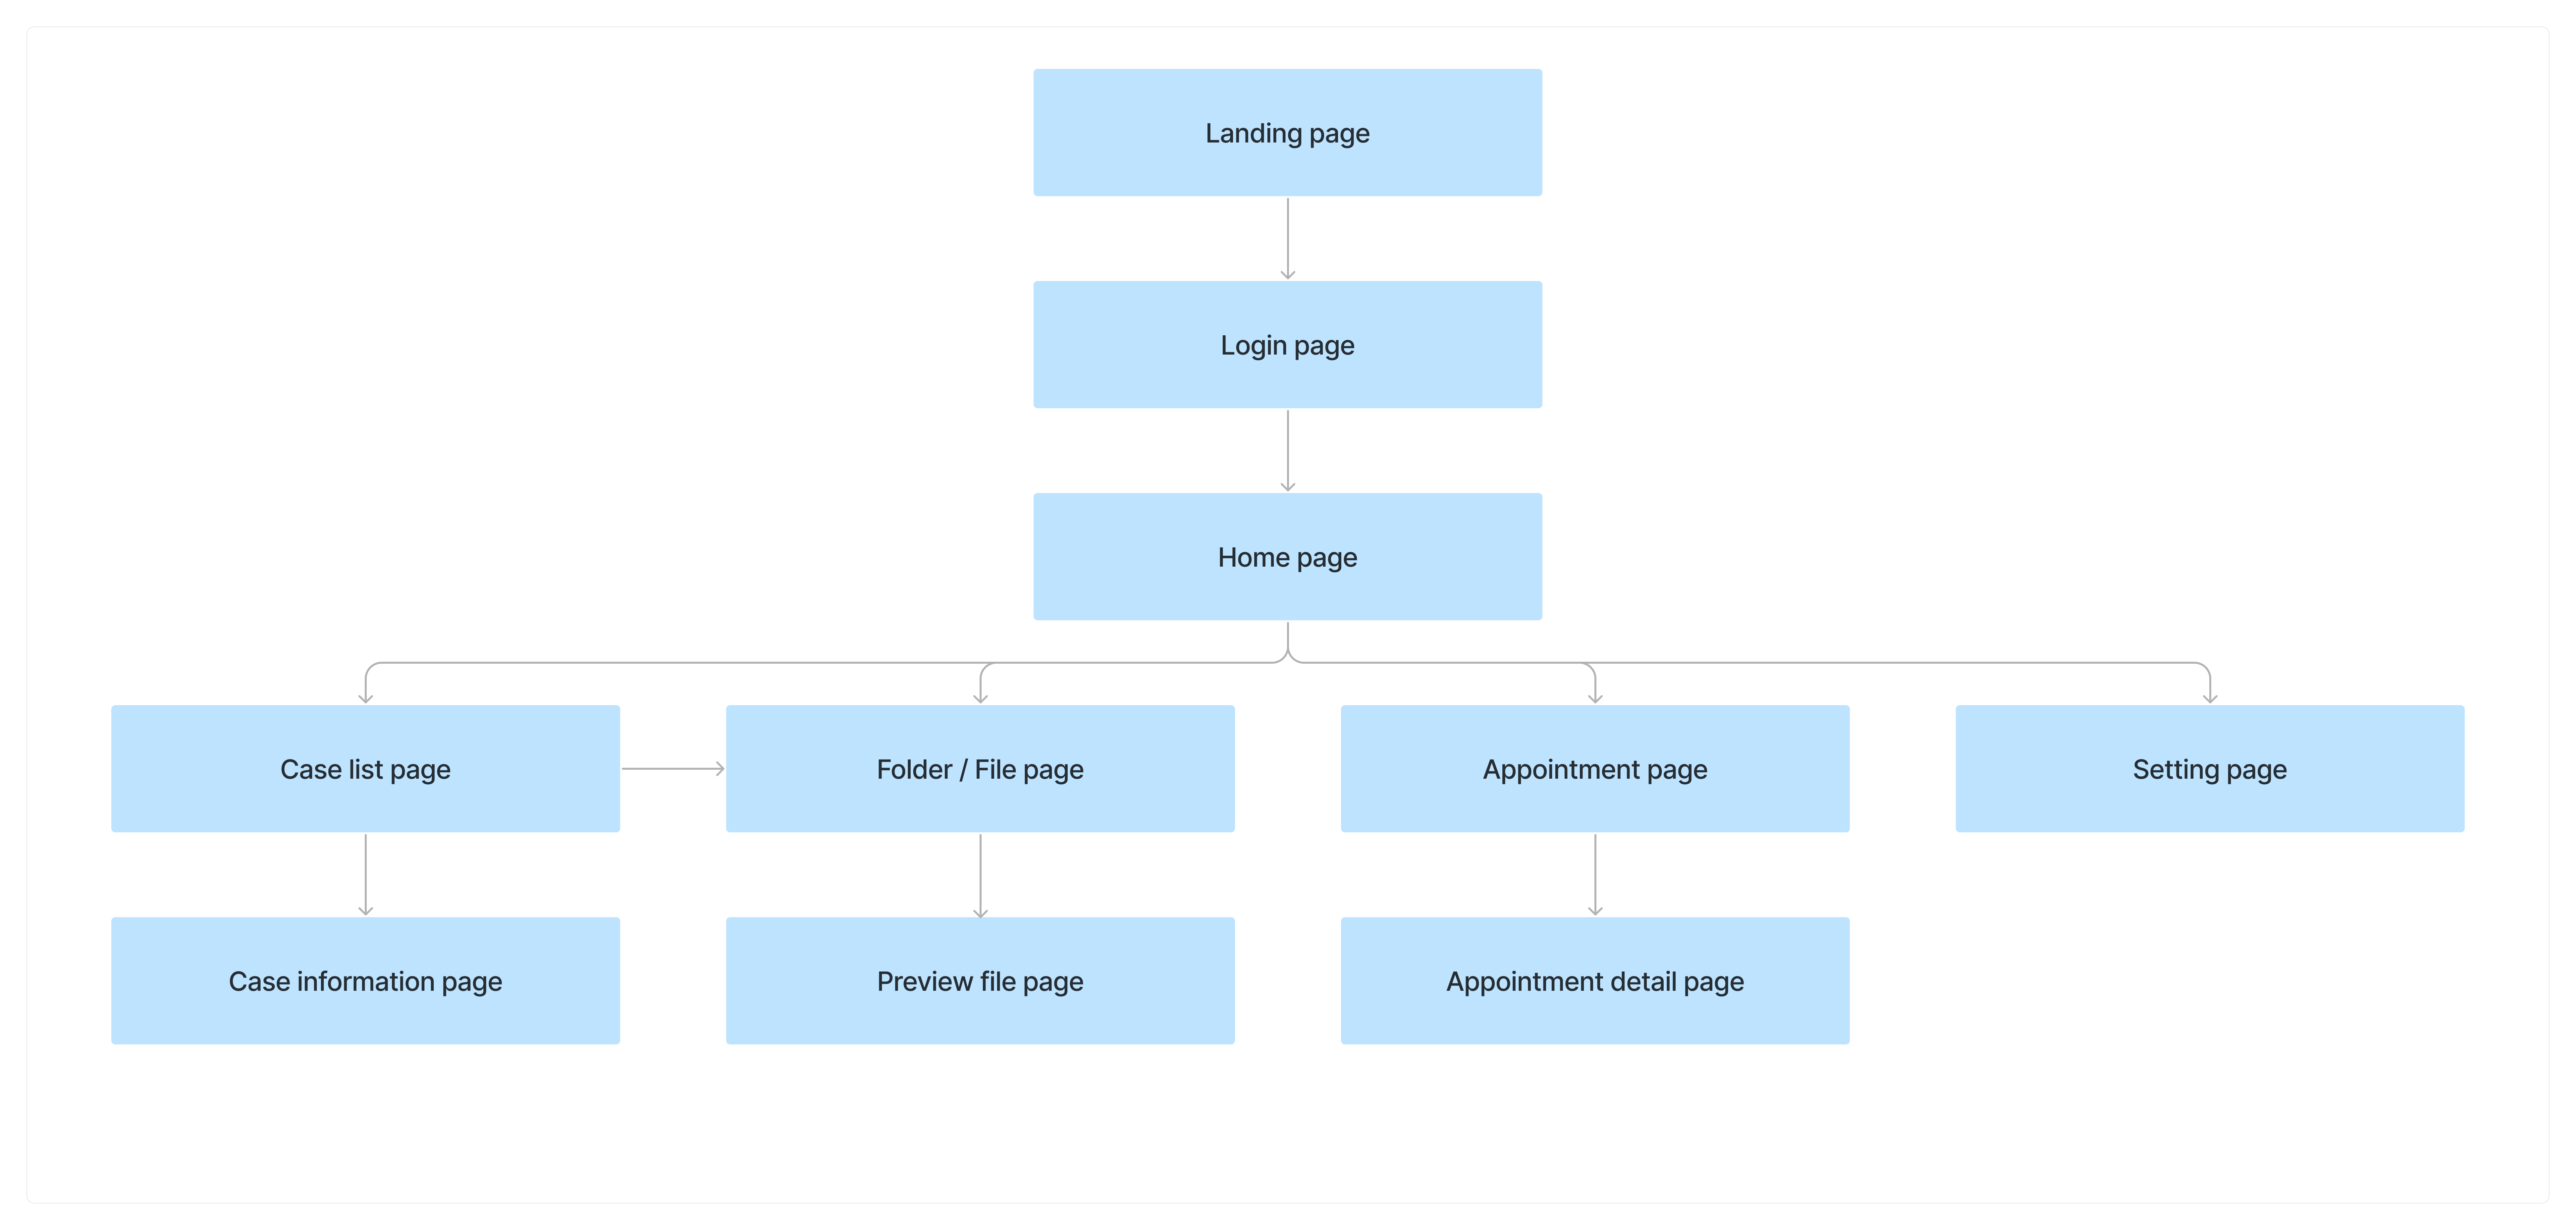
\includegraphics[width=13cm]{./assets/nav-map-lawyer.png}
    \caption{รูปแสดง Navigation map ของทนายความ}\label{fig:navMapLawyer}
\end{figure}

\clearpage
\newpage
\section{โครงสร้างฐานข้อมูล}
\hspace*{1cm}โครงสร้างฐานข้อมูลของเว็บแอปพลิเคชันแสดงดังรูป \ref{fig:erDiagram} โดยมีรายละเอียดของชนิดตัวแปรและคํา
อธิบายเพิ่มเติมดังตารางที่ \ref{tbl:dbFileType} - \ref{tbl:dbUser} ดังนี้
\begin{figure}[!ht]\centering
    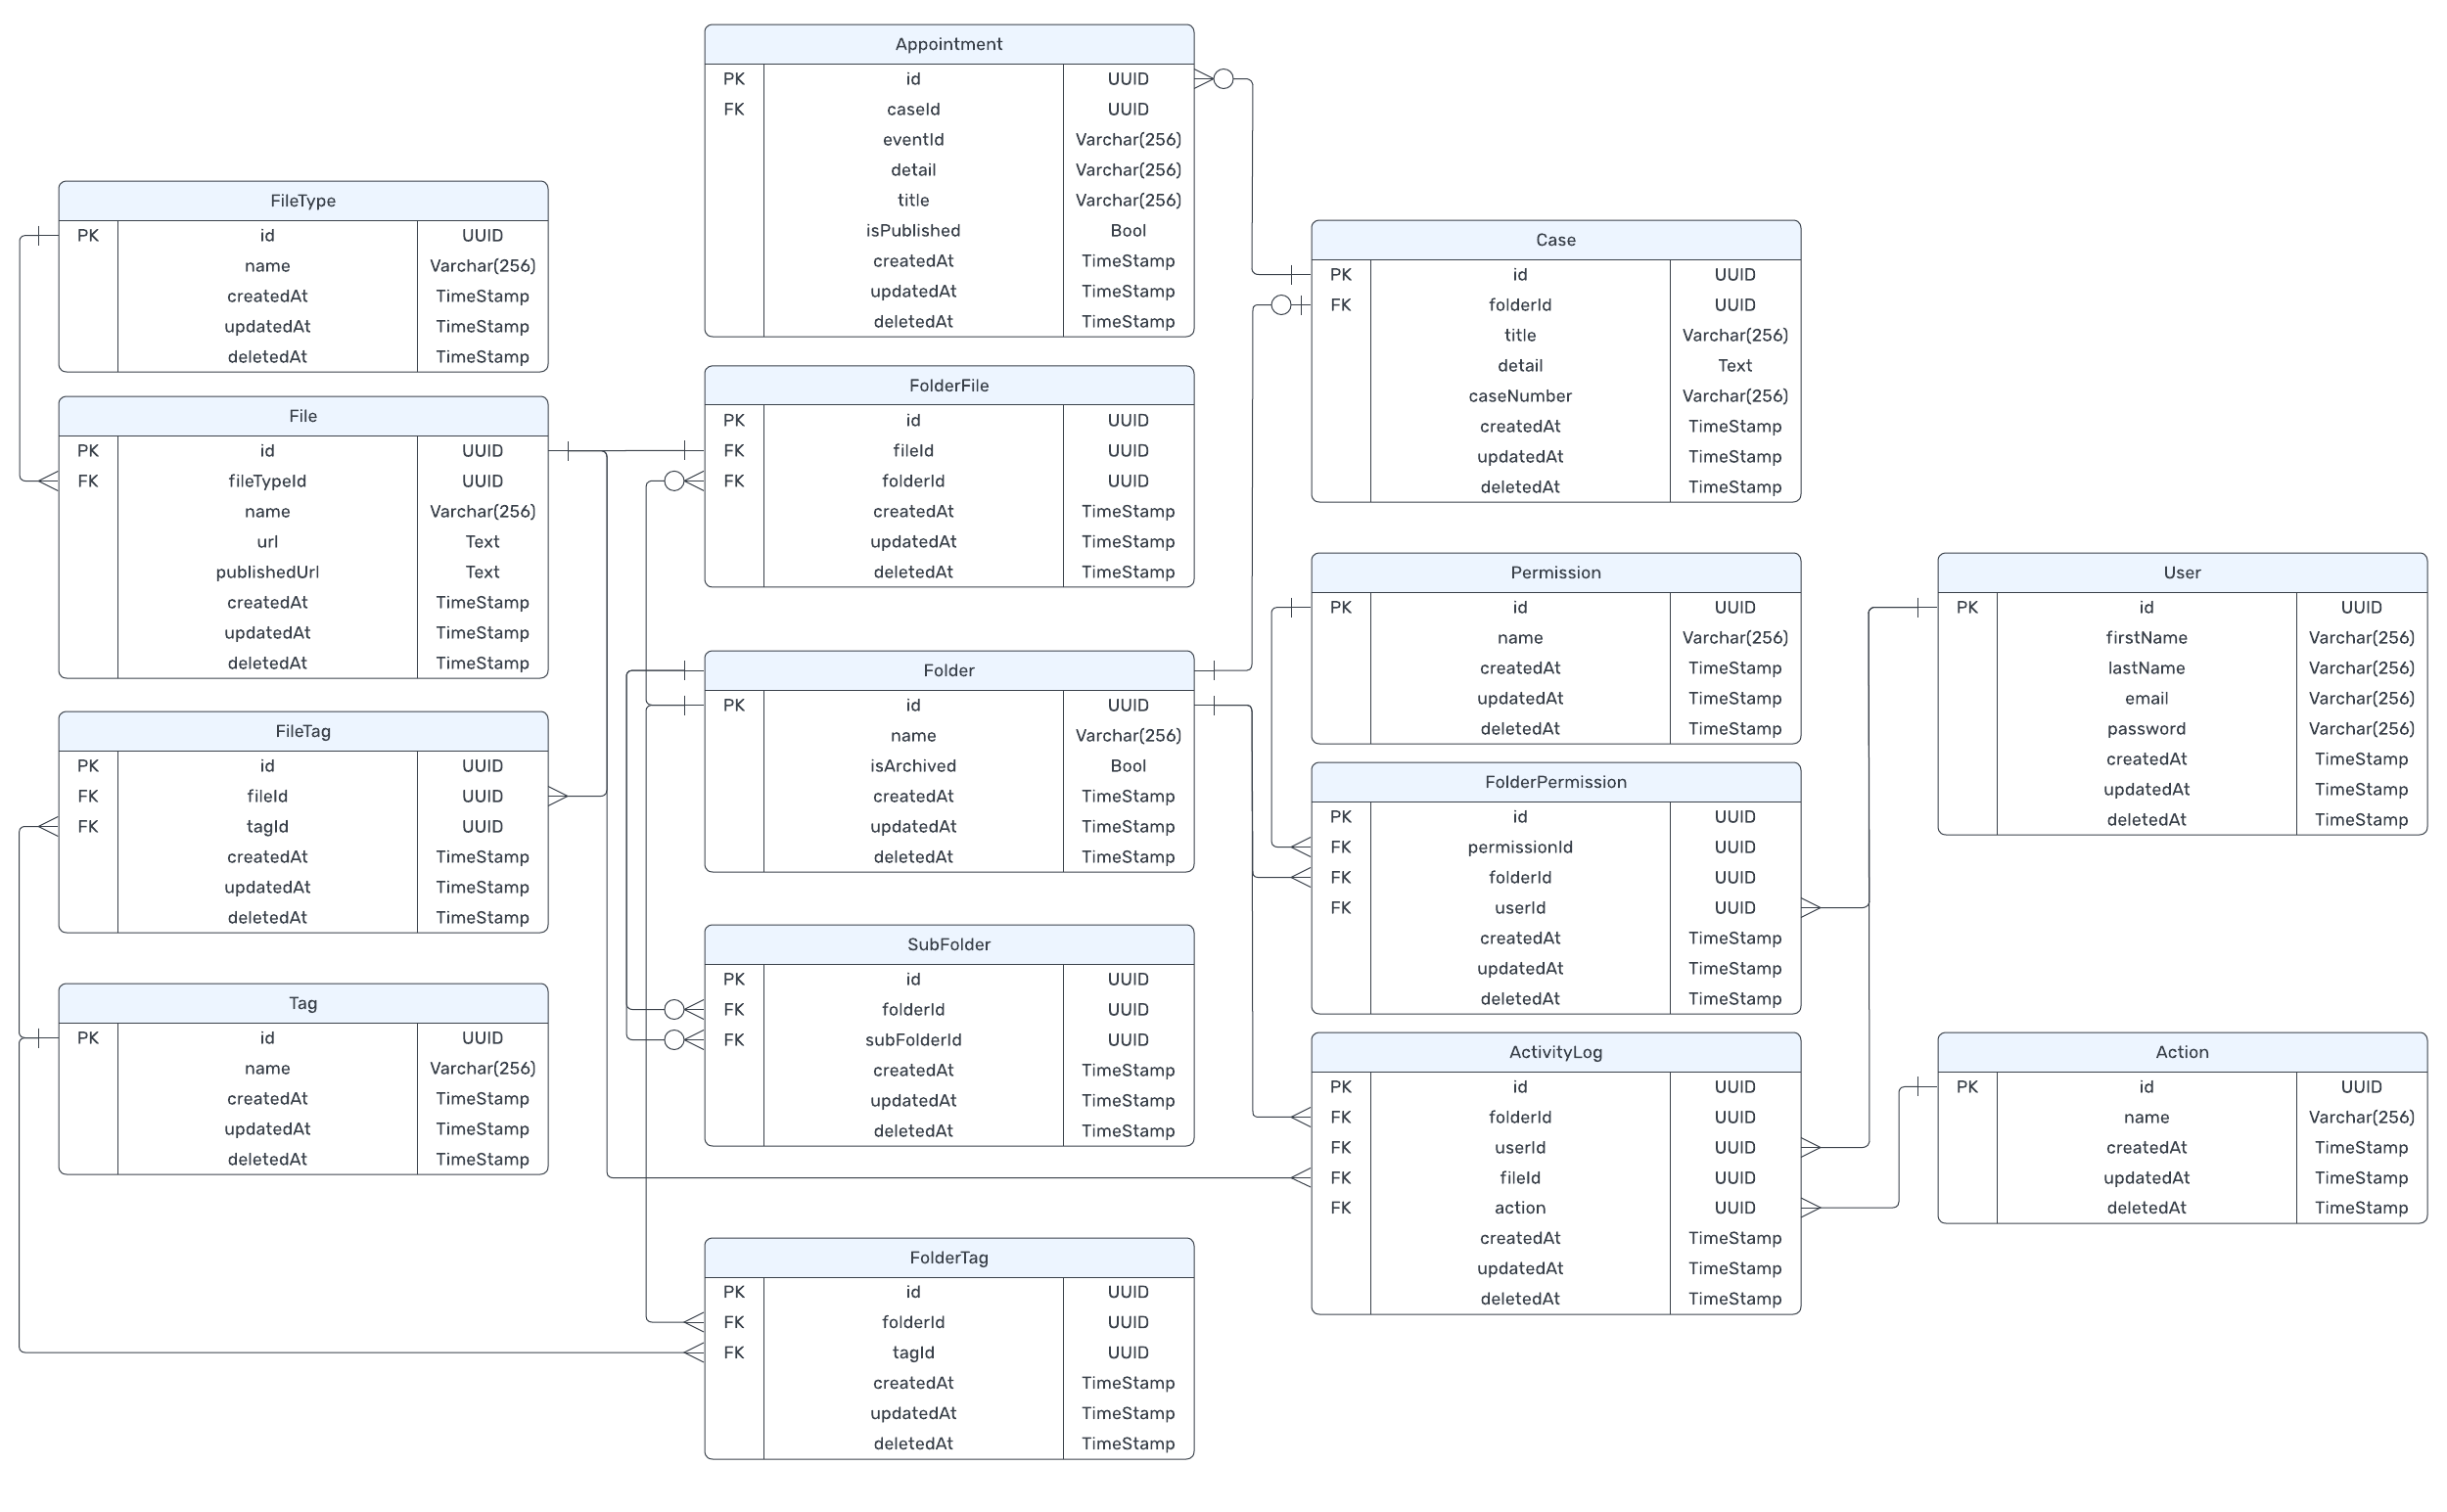
\includegraphics[width=15cm]{./assets/er-diagram.png}
    \caption{รูปแสดงโครงสร้างฐานข้อมูล}\label{fig:erDiagram}
\end{figure}
\begin{itemize}
\item \textbf{ตาราง FileType}\\
ตารางที่ใช้ในการบันทึกข้อมูล ประเภทของไฟล์ในระบบ เช่น ไฟล์ประเภทเอกสาร ไฟล์ประเภทรูปภาพ เป็นต้น โดยมีรายละเอียดดังตารางที่ \ref{tbl:dbFileType}
\begin{table}[!ht]
    \centering
    \begin{tabular}{|p{4cm}|p{2cm}|p{6cm}|}
    \hline
    \textbf{Attribute} & \textbf{Type} & \textbf{Description}   \\ \hline
    id                 & UUID          & ID ของประเภทไฟล์       \\ \hline
    name               & Varchar(256)   & ชื่อของประเภทของไฟล์   \\ \hline
    createdAt          & TimeStamp     & วันเวลาที่สร้าง        \\ \hline
    updatedAt          & TimeStamp     & วันเวลาที่อัพเดทล่าสุด \\ \hline
    deletedAt          & TimeStamp     & วันเวลาที่ลบ           \\ \hline
    \end{tabular}
    \caption{\centering  ตารางแสดงรายละเอียดของตาราง FileType} \label{tbl:dbFileType}
\end{table}


\item \textbf{ตาราง File}\\
ตารางที่ใช้ในการบันทึกข้อมูลรายละเอียดไฟล์ที่ได้จากผู้ใช้งาน โดยมีรายละเอียดดังตารางที่ \ref{tbl:dbFile}
\begin{table}[!ht]
    \centering
    \begin{tabular}{|p{4cm}|p{2cm}|p{6cm}|}
    \hline
    \textbf{Attribute} & \textbf{Type} & \textbf{Description}   \\ \hline
    id                 & UUID          & ID ของไฟล์                                                      \\ \hline
    name               & Varchar(256)   & ชื่อของประเภทของไฟล์                                            \\ \hline
    fileTypeId         & UUID          & ID ของประเภทของไฟล์                                             \\ \hline
    url                & text          & Url ของไฟล์ที่ได้จาก google storage                             \\ \hline
    publishedUrl       & text          & Url ของไฟล์ที่บุคคลที่ไม่ใช่ทนายใช้ในการเข้าถึงเอกสารและดาวโหลด \\ \hline
    createdAt          & TimeStamp     & วันเวลาที่สร้าง                                                 \\ \hline
    updatedAt          & TimeStamp     & วันเวลาที่อัพเดทล่าสุด                                          \\ \hline
    deletedAt          & TimeStamp     & วันเวลาที่ลบ                                                    \\ \hline
    \end{tabular}
    \caption{\centering  ตารางแสดงรายละเอียดของตาราง File} \label{tbl:dbFile}
\end{table}

\item \textbf{ตาราง Tag}\\
ตารางที่ใช้ในการบันทึกข้อมูลรายละเอียดของแท็กต่าง ๆ โดยมีรายละเอียดดังตารางที่ \ref{tbl:dbTag}
\begin{table}[!ht]
    \centering
    \begin{tabular}{|p{4cm}|p{2cm}|p{6cm}|}
    \hline
    \textbf{Attribute} & \textbf{Type} & \textbf{Description}   \\ \hline
    id                 & UUID          & ID ของ tag             \\ \hline
    name               & Varchar(256)   & ชื่อ tag               \\ \hline
    createdAt          & TimeStamp     & วันเวลาที่สร้าง        \\ \hline
    updatedAt          & TimeStamp     & วันเวลาที่อัพเดทล่าสุด \\ \hline
    deletedAt          & TimeStamp     & วันเวลาที่ลบ       \\ \hline
    \end{tabular}
    \caption{\centering  ตารางแสดงรายละเอียดของตาราง Tag} \label{tbl:dbTag}
\end{table}
\newpage
\item \textbf{ตาราง FileTag}\\
ตารางที่ใช้ในการบันทึกข้อมูลความสัมพันธ์ระหว่าง file กับ Tag โดยที่ว่า ใน 1 ไฟล์นั้นสามารถมีได้หลาย Tag โดยมีรายละเอียดดังตารางที่ \ref{tbl:dbFileTag}
\begin{table}[!ht]
    \centering
    \begin{tabular}{|p{4cm}|p{2cm}|p{6cm}|}
    \hline
    \textbf{Attribute} & \textbf{Type} & \textbf{Description}   \\ \hline
    id                 & UUID          & ID ของ file tag        \\ \hline
    fileId             & UUID          & ID ของ file            \\ \hline
    tagId              & UUID          & ID ของ tag             \\ \hline
    createdAt          & TimeStamp     & วันเวลาที่สร้าง        \\ \hline
    updatedAt          & TimeStamp     & วันเวลาที่อัพเดทล่าสุด \\ \hline
    deletedAt          & TimeStamp     & วันเวลาที่ลบ          \\ \hline
    \end{tabular}
    \caption{\centering  ตารางแสดงรายละเอียดของตาราง FileTag} \label{tbl:dbFileTag}
\end{table}

\item \textbf{ตาราง Folder}\\
ตารางที่ใช้ในการบันทึกข้อมูลรายละเอียดโฟลเดอร์โดยจะมี attribute ที่มีชื่อว่า isArchived มาใช้ในการบ่งบอกว่าโฟลเดอร์นี้สามารถใช้งานได้หรือไม่โดยมีรายละเอียดดังตารางที่ \ref{tbl:dbFolder}
\begin{table}[!ht]
    \centering
    \begin{tabular}{|p{4cm}|p{2cm}|p{6cm}|}
    \hline
    \textbf{Attribute} & \textbf{Type} & \textbf{Description}   \\ \hline
    id        & UUID        & ID ของ folder          \\ \hline
    name      & Varchar(256) & ชื่อ folder            \\ \hline
    isArchived         & Boolean          & เก็บถาวรหรือเป็น attribute ที่บ่งบอกถึงสถานะการใช้งานว่าใช้ได้หรือไม่ \\ \hline
    createdAt & TimeStamp   & วันเวลาที่สร้าง        \\ \hline
    updatedAt & TimeStamp   & วันเวลาที่อัพเดทล่าสุด \\ \hline
    deletedAt & TimeStamp   & วันเวลาที่ลบ             \\ \hline
    \end{tabular}
    \caption{\centering  ตารางแสดงรายละเอียดของตาราง Folder} \label{tbl:dbFolder}
\end{table}

\item \textbf{ตาราง FolderFile}\\
ตารางที่ใช้ในการบันทึกข้อมูลว่าโฟลเดอร์นั้น ๆ เก็บไฟล์อะไรไว้บ้าง โดยมีรายละเอียดดังตารางที่  \ref{tbl:dbFolderFile}
\begin{table}[!ht]
    \centering
    \begin{tabular}{|p{4cm}|p{2cm}|p{6cm}|}
    \hline
    \textbf{Attribute} & \textbf{Type} & \textbf{Description}   \\ \hline
    id        & UUID      & ID ของ folder file     \\ \hline
    flieId    & UUID      & ID ของ file            \\ \hline
    folderId  & UUID      & ID ของ folder          \\ \hline
    createdAt & TimeStamp & วันเวลาที่สร้าง        \\ \hline
    updatedAt & TimeStamp & วันเวลาที่อัพเดทล่าสุด \\ \hline
    deletedAt & TimeStamp & วันเวลาที่ลบ              \\ \hline
    \end{tabular}
    \caption{\centering  ตารางแสดงรายละเอียดของตาราง FolderFile} \label{tbl:dbFolderFile}
\end{table}
\newpage
\item \textbf{ตาราง SubFolder}\\
ตารางที่ใช้ในการบันทึกข้อมูลรายละเอียดไฟล์โดยมีรายละเอียดดังตารางที่ \ref{tbl:dbSubFolder}
\begin{table}[!ht]
    \centering
    \begin{tabular}{|p{4cm}|p{2cm}|p{6cm}|}
    \hline
    \textbf{Attribute} & \textbf{Type} & \textbf{Description}   \\ \hline
    id          & UUID      & ID ของ record                \\ \hline
    folderId    & UUID      & ID ของโฟลเดอร์ที่อยู่ด้านนอก \\ \hline
    subFolderId & UUID      & ID ของโฟลเดอร์ที่อยู่ด้านใน  \\ \hline
    createdAt   & TimeStamp & วันเวลาที่สร้าง              \\ \hline
    updatedAt   & TimeStamp & วันเวลาที่อัพเดทล่าสุด       \\ \hline
    deletedAt   & TimeStamp & วันเวลาที่ลบ                \\ \hline  
    \end{tabular}
    \caption{\centering  ตารางแสดงรายละเอียดของตาราง SubFolder} \label{tbl:dbSubFolder}
\end{table}

\item \textbf{ตาราง FolderTag}\\
ตารางที่ใช้ในการบันทึกข้อมูลรายละเอียดไฟล์โดยมีรายละเอียดดังตารางที่ \ref{tbl:dbFolderTag}
\begin{table}[!ht]
    \centering
    \begin{tabular}{|p{4cm}|p{2cm}|p{6cm}|}
    \hline
    \textbf{Attribute} & \textbf{Type} & \textbf{Description}   \\ \hline
    id        & UUID      & ID ของ record          \\ \hline
    folderId  & UUID      & ID ของ folder          \\ \hline
    tagId     & UUID      & ID ของ tag             \\ \hline
    createdAt & TimeStamp & วันเวลาที่สร้าง        \\ \hline
    updatedAt & TimeStamp & วันเวลาที่อัพเดทล่าสุด \\ \hline
    deletedAt & TimeStamp & วันเวลาที่ลบ     \\ \hline
    \end{tabular}
    \caption{\centering  ตารางแสดงรายละเอียดของตาราง FolderTag} \label{tbl:dbFolderTag}
\end{table}

\item \textbf{ตาราง Case}\\
ตารางที่ใช้ในการบันทึกข้อมูลรายละเอียดคดีในแต่ละคดี โดยมีรายละเอียดดังตารางที่ \ref{tbl:dbCase}
\begin{table}[!ht]
    \centering
    \begin{tabular}{|p{4cm}|p{2cm}|p{6cm}|}
    \hline
    \textbf{Attribute} & \textbf{Type} & \textbf{Description}   \\ \hline
    id         & UUID        & ID ของ case                 \\ \hline
    folderId   & UUID        & ID ของ folder ที่เชื่อมอยู่ \\ \hline
    title      & Varchar(256) & ชื่อคดี                     \\ \hline
    detail     & text        & รายละเอียดคดี               \\ \hline
    caseNumber & Varchar(256) & เลขคดี                      \\ \hline
    createdAt  & TimeStamp   & วันเวลาที่สร้าง             \\ \hline
    updatedAt  & TimeStamp   & วันเวลาที่อัพเดทล่าสุด      \\ \hline
    deletedAt  & TimeStamp   & วันเวลาที่ลบ     \\ \hline
    \end{tabular}
    \caption{\centering  ตารางแสดงรายละเอียดของตาราง Case} \label{tbl:dbCase}
\end{table}

\newpage
\item \textbf{ตาราง Appointment}\\
ตารางที่ใช้ในการบันทึกการนัดหมาย โดยจะมี attribute isPublished มาใช้ในการบ่งบอกว่า นัดหมายในครั้งนี้สามารถเปิดเผยสู่สาธารณะได้หรือไม่ และมี eventId ที่ได้มาจากการสร้าง event ผ่าน Google calendar api โดยมีรายละเอียดดังตารางที่  \ref{tbl:dbAppointment}
\begin{table}[!ht]
    \centering
    \begin{tabular}{|p{4cm}|p{2cm}|p{6cm}|}
    \hline
    \textbf{Attribute} & \textbf{Type} & \textbf{Description}   \\ \hline
    id          & UUID        & ID ของ appointment                        \\ \hline
    caseId      & UUID        & ID ของ case                               \\ \hline
    eventId     & Varchar(256) & ID ของ event ที่ใช้ใน google calendar api \\ \hline
    detail      & Varchar(256) & รายละเอียดของการนัดหมาย                   \\ \hline
    title       & Varchar(256) & ชื่อของการนัดหมาย                         \\ \hline
    isPublished & Boolean        & เปิดเผยสู่สาธารณะหรือไม่                  \\ \hline
    createdAt   & TimeStamp   & วันเวลาที่สร้าง                           \\ \hline
    updatedAt   & TimeStamp   & วันเวลาที่อัพเดทล่าสุด                    \\ \hline
    deletedAt   & TimeStamp   & วันเวลาที่ลบ             \\ \hline
    \end{tabular}
    \caption{\centering  ตารางแสดงรายละเอียดของตาราง Appointment} \label{tbl:dbAppointment}
\end{table}


\item \textbf{ตาราง Permission}\\
ตารางที่ใช้ในการบันทึกข้อมูลรายสิทธิในการเข้าถึงที่มีอยู่ในระบบ โดยมีรายละเอียดดังตารางที่ \ref{tbl:dbPermission}
\begin{table}[!ht]
    \centering
    \begin{tabular}{|p{4cm}|p{2cm}|p{6cm}|}
    \hline
    \textbf{Attribute} & \textbf{Type} & \textbf{Description}   \\ \hline
    id        & UUID        & ID ของ permission      \\ \hline
    name      & Varchar(256) & ชื่อของ permission     \\ \hline
    createdAt & TimeStamp   & วันเวลาที่สร้าง        \\ \hline
    updatedAt & TimeStamp   & วันเวลาที่อัพเดทล่าสุด \\ \hline
    deletedAt & TimeStamp   & วันเวลาที่ลบ                \\ \hline
    \end{tabular}
    \caption{\centering  ตารางแสดงรายละเอียดของตาราง Permission} \label{tbl:dbPermission}
\end{table}

\item \textbf{ตาราง FolderPermission}\\
ตารางที่ใช้ในการบันทึกข้อมูลรายละเอียดไฟล์ที่เชื่อมความสัมพันธ์ระหว่างสิทธิของผู้ใช้งานกับโฟลเดอร์ โดยมีรายละเอียดดังตารางที่ \ref{tbl:dbFolderPermission}
\begin{table}[!ht]
    \centering
    \begin{tabular}{|p{4cm}|p{2cm}|p{6cm}|}
    \hline
    \textbf{Attribute} & \textbf{Type} & \textbf{Description}   \\ \hline
    id           & UUID      & ID ของ folder appointment \\ \hline
    permissionId & UUID      & ID ของ permission         \\ \hline
    folderId     & UUID      & ID ของ folder             \\ \hline
    userId       & UUID      & ID ของ user               \\ \hline
    createdAt    & TimeStamp & วันเวลาที่สร้าง           \\ \hline
    updatedAt    & TimeStamp & วันเวลาที่อัพเดทล่าสุด    \\ \hline
    deletedAt    & TimeStamp & วันเวลาที่ลบ            \\ \hline
    \end{tabular}
    \caption{\centering  ตารางแสดงรายละเอียดของตาราง FolderPermission} \label{tbl:dbFolderPermission}
\end{table}
\newpage
\item \textbf{ตาราง ActivityLog}\\
ตารางที่ใช้ในการบันทึกข้อมูลการอัพเดทไฟล์ที่เกิดขึ้นในแต่ละโฟลเดอร์ โดยมีรายละเอียดดังตารางที่ \ref{tbl:dbActivityLog}
\begin{table}[!ht]
    \centering
    \begin{tabular}{|p{4cm}|p{2cm}|p{6cm}|}
    \hline
    \textbf{Attribute} & \textbf{Type} & \textbf{Description}   \\ \hline
    id        & UUID      & ID ของ activity log                 \\ \hline
    folderId  & UUID      & ID ของ folder ที่ถูกทำการอัพเดทไฟล์ \\ \hline
    userId    & UUID      & ID ของ user ที่ทำการอัพเดทไฟล์      \\ \hline
    flieId    & UUID      & ID ของ file ที่ถูกทำการอัพเดท       \\ \hline
    actionId  & UUID      & ID ของ action ที่ทำ                 \\ \hline
    createdAt & TimeStamp & วันเวลาที่สร้าง                     \\ \hline
    updatedAt & TimeStamp & วันเวลาที่อัพเดทล่าสุด              \\ \hline
    deletedAt & TimeStamp & วันเวลาที่ลบ                      \\ \hline
    \end{tabular}
    \caption{\centering  ตารางแสดงรายละเอียดของตาราง ActivityLog} \label{tbl:dbActivityLog}
\end{table}
\item \textbf{ตาราง Action}\\
ตารางที่ใช้ในการบันทึกข้อมูลรายละเอียดของการทำ activity เช่น สร้าง อัพเดท ลบ โดยมีรายละเอียดดังตารางที่ \ref{tbl:dbAction}
\begin{table}[!ht]
    \centering
    \begin{tabular}{|p{4cm}|p{2cm}|p{6cm}|}
    \hline
    \textbf{Attribute} & \textbf{Type} & \textbf{Description}   \\ \hline
    id        & UUID        & ID ของ action          \\ \hline
    name      & Varchar(256) & ชื่อของ action         \\ \hline
    createdAt & TimeStamp   & วันเวลาที่สร้าง        \\ \hline
    updatedAt & TimeStamp   & วันเวลาที่อัพเดทล่าสุด \\ \hline
    deletedAt & TimeStamp   & วันเวลาที่ลบ          \\ \hline    
    \end{tabular}
    \caption{\centering  ตารางแสดงรายละเอียดของตาราง Action} \label{tbl:dbAction}
\end{table}

\item \textbf{ตาราง User}\\
ตารางที่ใช้ในการบันทึกข้อมูลรายละเอียดผู้ใช้งาน โดยมีรายละเอียดดังตารางที่ \ref{tbl:dbUser}
\begin{table}[!ht]
    \centering
    \begin{tabular}{|p{4cm}|p{2cm}|p{6cm}|}
    \hline
    \textbf{Attribute} & \textbf{Type} & \textbf{Description}   \\ \hline
    id        & UUID        & ID ของ user            \\ \hline
    firstName & Varchar(256) & ชื่อจริง               \\ \hline
    lastName  & Varchar(256) & นามสกุล                \\ \hline
    email     & Varchar(256) & อีเมล์                 \\ \hline
    password  & Varchar(256) & รหัสผ่าน               \\ \hline
    createdAt & TimeStamp   & วันเวลาที่สร้าง        \\ \hline
    updatedAt & TimeStamp   & วันเวลาที่อัพเดทล่าสุด \\ \hline
    deletedAt & TimeStamp   & วันเวลาที่ลบ                \\ \hline
    \end{tabular}
    \caption{\centering  ตารางแสดงรายละเอียดของตาราง User} \label{tbl:dbUser}
\end{table}
\end{itemize}
% \clearpage
\newpage
\section{Use case diagram}
\begin{figure}[!ht]\centering
    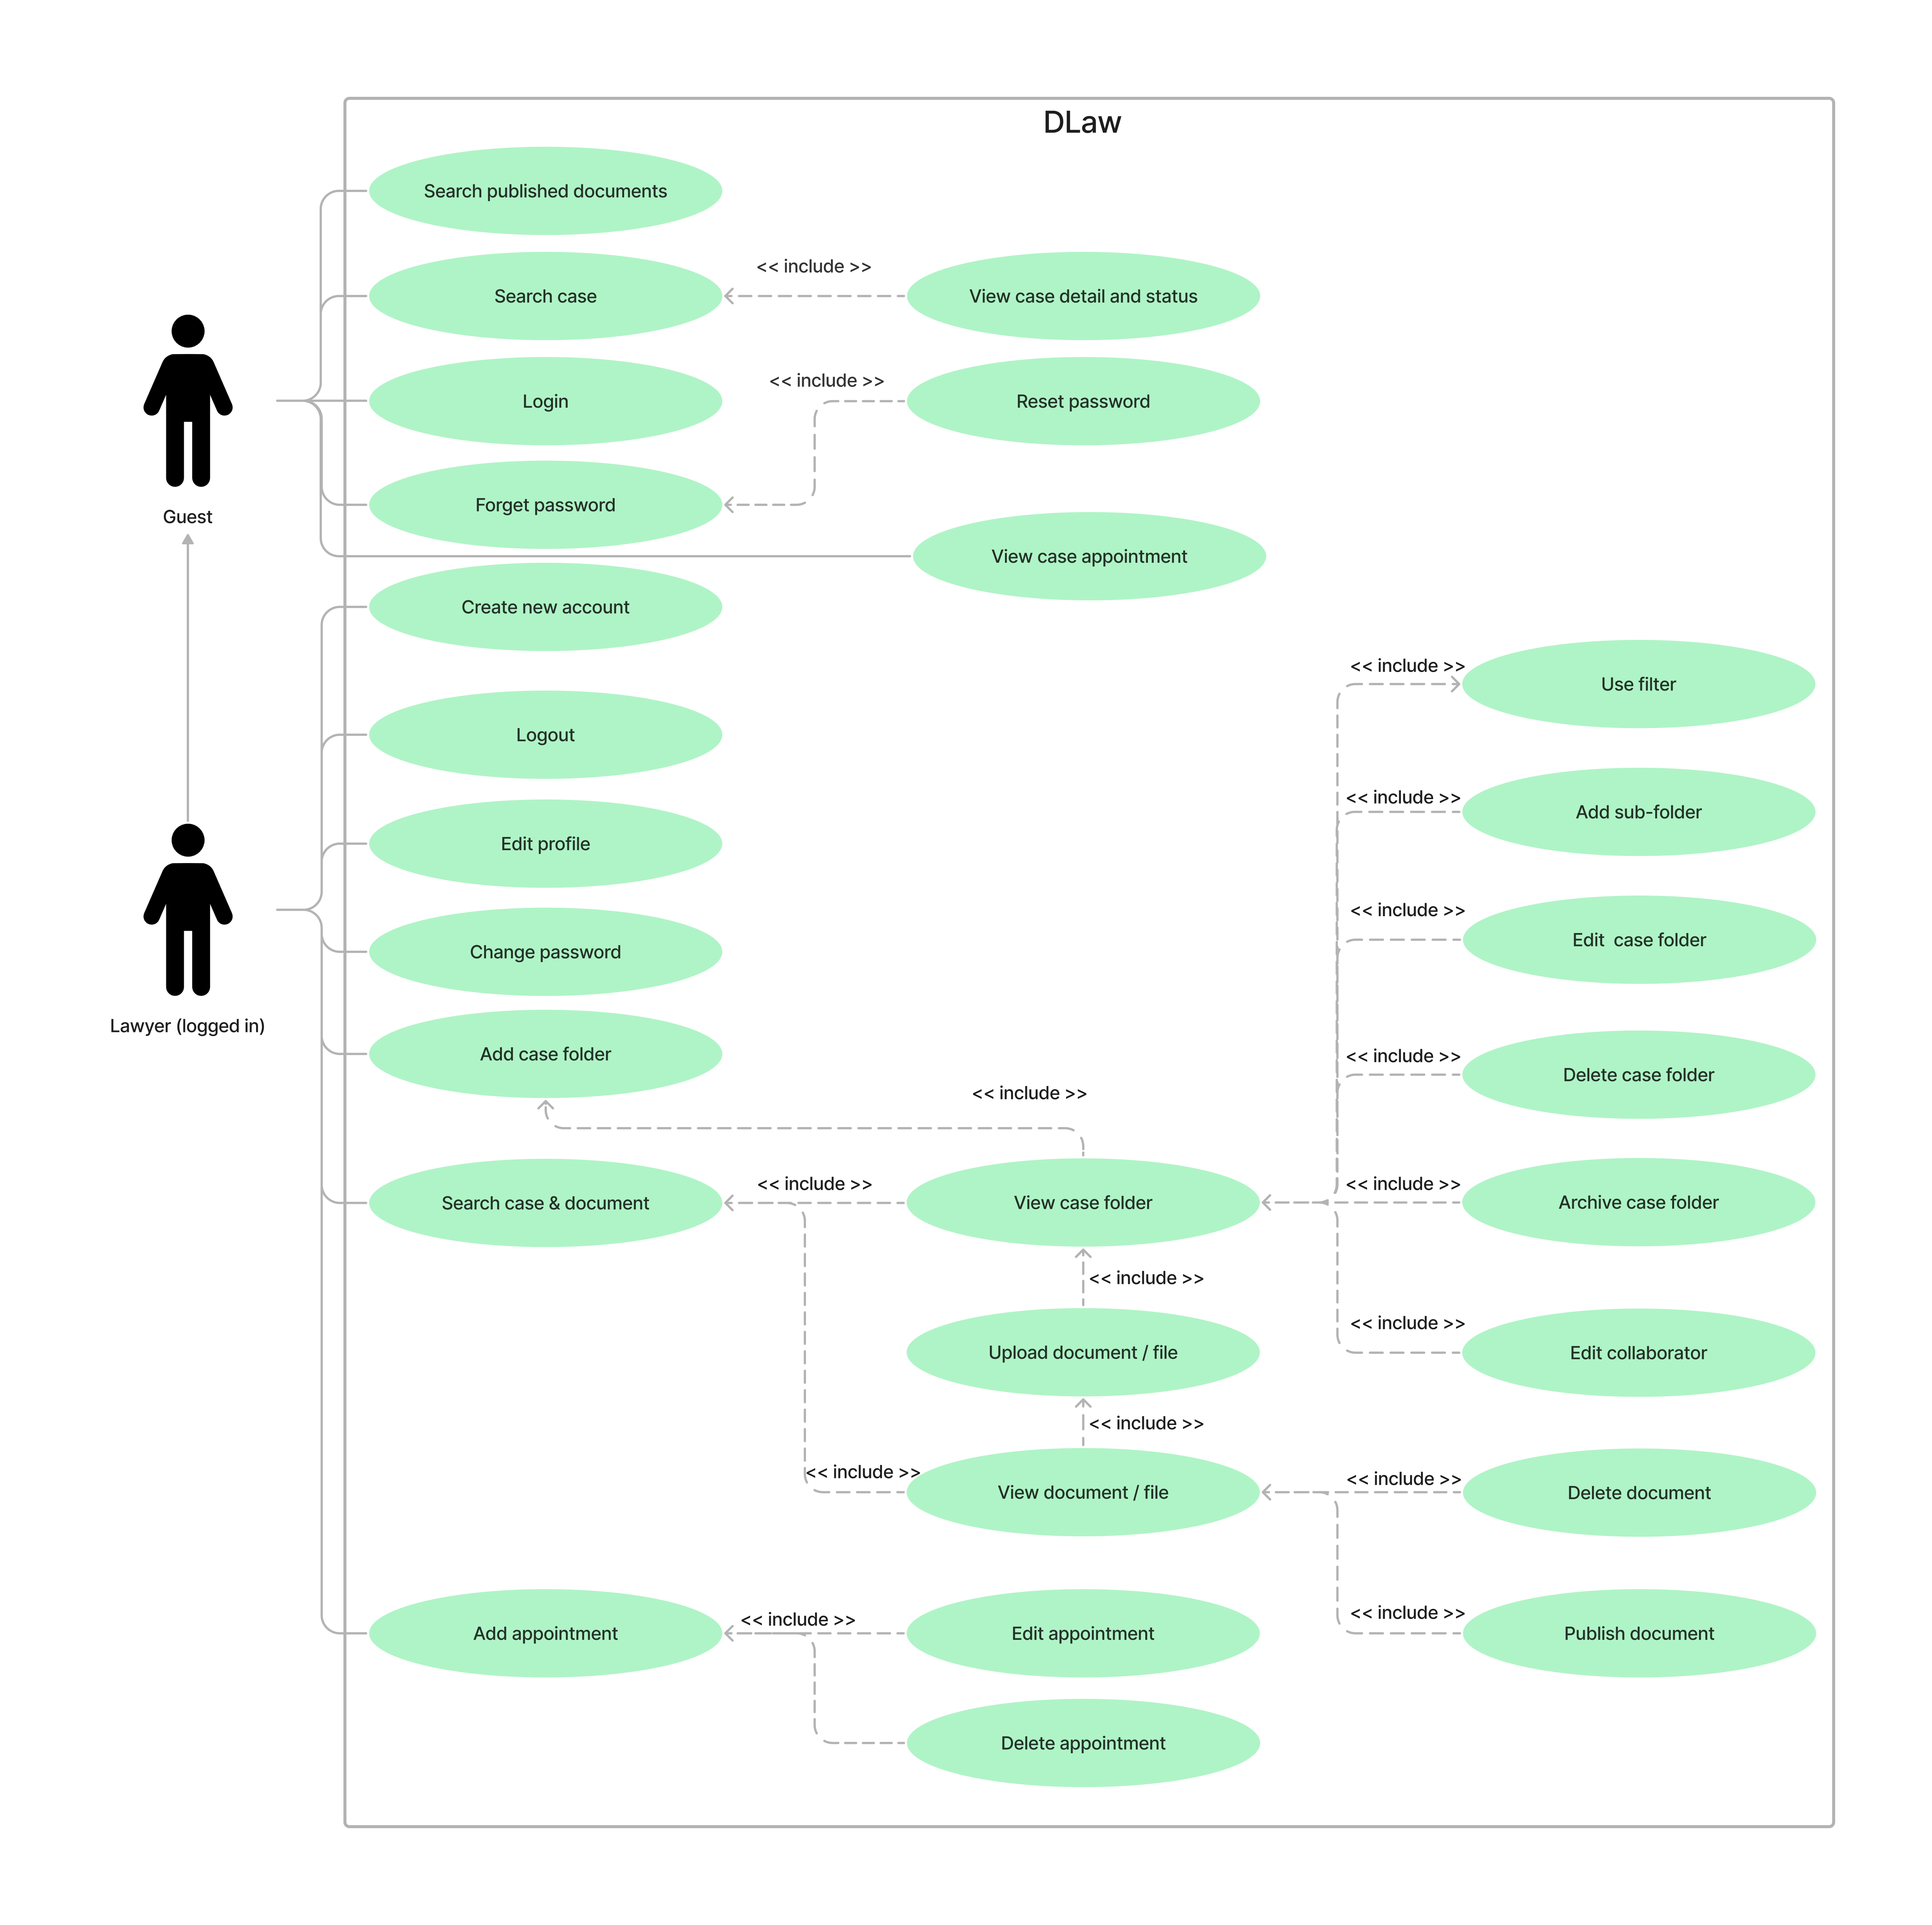
\includegraphics[width=16cm]{./assets/use-case-diagram.png}
    \caption{รูปแสดง Use case diagram แสดงการทำงานของระบบ}\label{fig:usecaseDiagram}
\end{figure}

\hspace*{1cm}จากรูปที่ \ref{fig:usecaseDiagram} แสดง Use case digram การทำงานจะถูกแบ่งออกเป็น 2 ส่วน คือ ส่วนของผู้ใช้งานทั่วไป และ ส่วนของทนาย ซึ่งมีความแตกต่างกัน คือ 
\begin{itemize}
    \item ผู้ใช้งานทั่วไปสามารถเข้าถึงเอกสารหรือนัดหมายที่ถูกเปิดเผยสู่สาธารณะได้ 
    \item ผู้ใช้งานที่เข้าสู่ระบบหรือ ทนายสามารเข้าถึงการจัดการเอกสารต่าง ๆ และนัดหมายที่ตนเองมีสิทธิ์ในคดีนั้น ๆ ได้ และฟังก์ชันพื้นฐานเช่น การเปลี่ยนรหัสผ่าน การแก้ไขโปรไฟล์ และสุดท้ายคือ การเพิ่ม user ใหม่ 
\end{itemize}


\clearpage
\section{Use case narrative}
\hspace*{1cm}จากรูปที่ \ref{fig:usecaseDiagram} ซึ่งมี usecase ต่าง ๆ โดยจะมีการอธิบายรายละเอียดเพิ่มเติม ดังนี้
\begin{itemize}
    \item \textbf{Search case }\\
    
    \begin{table}[!ht]
        \centering
        \begin{tabular}{|p{5cm}|p{10cm}|}
            \hline
            \multicolumn{1}{|l|}{Use case}      & Search case                        \\ \hline
            \multicolumn{1}{|l|}{Actor}         & Guest                                  \\ \hline
            \multicolumn{1}{|l|}{Goal}          & ผู้ใช้สามารถเห็นคดีที่ต้องการค้นหา \\ \hline
            \multicolumn{1}{|l|}{Pre-condition} & -                                      \\ \hline
            \multicolumn{1}{|l|}{Flow of event} &
              \begin{tabular}[c]{@{}l@{}}1. ผู้ใช้กดเมนูค้นหาคดี\\ 2. ผู้ใช้กรอกหมายเลขคดีดำหรือหมายเลขคดีแดง\\ 3. ผู้ใช้กดปุ่มค้นหา\\ 4. ระบบตรวจสอบข้อมูลและถูกต้อง\\ 5. ระบบดึงข้อมูลจาก API \\ 6. ระบบแสดงรายละเอียดคดี \end{tabular} \\ \hline
            \multicolumn{2}{|l|}{Extension scenario (a)}                                 \\ \hline
            \multicolumn{2}{|l|}{\begin{tabular}[c]{@{}l@{}}4a. ระบบตรวจสอบไม่ถูกต้อง\\ 5a. เว็บแสดงข้อความแจ้งเตือน\end{tabular}} \\ \hline
            \multicolumn{2}{|l|}{Extension scenario (b)}                                 \\ \hline
            \multicolumn{2}{|l|}{\begin{tabular}[c]{@{}l@{}}5b. ระบบดึงข้อมูลจาก API ไม่สำเร็จ\\ 6b. เว็บแสดงข้อความแจ้งเตือน\end{tabular}} \\ \hline
        \end{tabular}

        \caption{\centering  ตารางแสดงรายละเอียด Use case Search case } \label{tbl:usecaseSearchCase}
    \end{table}
    \item \textbf{View case detail and status}
     \begin{table}[!ht]
        \centering
        \begin{tabular}{|p{5cm}|p{10cm}|}
            \hline
            \multicolumn{1}{|l|}{Use case}      & View case detail and status                        \\ \hline
            \multicolumn{1}{|l|}{Actor}         & Guest                                  \\ \hline
            \multicolumn{1}{|l|}{Goal}          & ผู้ใช้สามารถเห็นรายละเอียดคดีเพิ่มเติม \\ \hline
            \multicolumn{1}{|l|}{Pre-condition} & ผู้ใช้ทำการค้นหาคดีพบ                                      \\ \hline
            \multicolumn{1}{|l|}{Flow of event} &
              \begin{tabular}[c]{@{}l@{}}1.กดบริเวณคดี\\ 2.ระบบแสดงรายละเอียดเพิ่มเติม  \end{tabular} \\ \hline
        \end{tabular}

        \caption{\centering  ตารางแสดงรายละเอียด Use case View case detail and status } \label{tbl:usecaseViewCaseDetail}
    \end{table}
    \newpage
    \item \textbf{View case appointment}
    \begin{table}[!ht]
        \centering
        \begin{tabular}{|p{5cm}|p{10cm}|}
            \hline
            \multicolumn{1}{|l|}{Use case}      & View case appointment                        \\ \hline
            \multicolumn{1}{|l|}{Actor}         & Guest                                  \\ \hline
            \multicolumn{1}{|l|}{Goal}          & ผู้ใช้สามารถเห็นรายละเอียดการนัดหมายที่ได้รับการเผยแพร่ \\ \hline
            \multicolumn{1}{|l|}{Pre-condition} & -                                      \\ \hline
            \multicolumn{1}{|l|}{Flow of event} &
              \begin{tabular}[c]{@{}l@{}}1. ผู้ใช้กดเมนู นัดหมาย \\2. ระบบทำการดึงข้อมูลจาก Database \\ 3. ระบบแสดงการนัดหมายที่ทำการเผยแพร่  \end{tabular} \\ \hline
        \end{tabular}

        \caption{\centering  ตารางแสดงรายละเอียด Use case View case appointment } \label{tbl:usecaseViewCaseAppointment}
    \end{table} 
    \item \textbf{Forget password}
    \begin{table}[!ht]
        \centering
        \begin{tabular}{|p{5cm}|p{10cm}|}
            \hline
            \multicolumn{1}{|l|}{Use case}      & Forget password                        \\ \hline
            \multicolumn{1}{|l|}{Actor}         & Guest                                  \\ \hline
            \multicolumn{1}{|l|}{Goal}          & ผู้ใช้ได้รับลิงค์สำหรับ reset password \\ \hline
            \multicolumn{1}{|l|}{Pre-condition} & -                                      \\ \hline
            \multicolumn{1}{|l|}{Flow of event} &
              \begin{tabular}[c]{@{}l@{}}1. ผู้ใช้กดปุ่ม Forget password\\ 2. ผู้ใช้กรอก Email\\ 3. ผู้ใช้กดยืนยัน\\ 4. ระบบตรวจสอบข้อมูลและถูกต้อง\\ 5. ลิงค์สำหรับ reset password ถูกส่งผ่านทางอีเมล์\end{tabular} \\ \hline
            \multicolumn{2}{|l|}{Extension scenario (a)}                                 \\ \hline
            \multicolumn{2}{|l|}{\begin{tabular}[c]{@{}l@{}}4a. ระบบตรวจสอบไม่ถูกต้อง\\ 5a. เว็บแสดงข้อความแจ้งเตือน\end{tabular}} \\ \hline
        \end{tabular}

        \caption{\centering  ตารางแสดงรายละเอียด Use case Forget password } \label{tbl:usecaseForgetPassword}
    \end{table}
    \item \textbf{Reset password}
    \begin{table}[!ht]
        \centering
        \begin{tabular}{|p{5cm}|p{10cm}|}
            \hline
            \multicolumn{1}{|l|}{Use case}      & Reset password                                     \\ \hline
            \multicolumn{1}{|l|}{Actor}         & Guest                                              \\ \hline
            \multicolumn{1}{|l|}{Goal}          & ผู้ใช้เปลี่ยนรหัสผ่านได้                           \\ \hline
            \multicolumn{1}{|l|}{Pre-condition} & ผู้ใช้ต้องได้รับลิงค์ reset password ผ่านทางอีเมล์ \\ \hline
            \multicolumn{1}{|l|}{Flow of event} &
            \begin{tabular}[c]{@{}l@{}}1. ผู้ใช้กดลิงค์ reset password ผ่านทางอีเมล์\\ 2. ผู้ใช้กรอก New password\\ 3. ผู้ใช้กรอก Confirm password\\ 4. ผู้ใช้กดยืนยัน\\ 5. ระบบทำการแก้ไขข้อมูล\\ 6. ผู้ใช้เปลี่ยนรหัสผ่านสำเร็จ\end{tabular} \\ \hline
            \multicolumn{2}{|l|}{Extension scenario (a)}                                             \\ \hline
            \multicolumn{2}{|l|}{\begin{tabular}[c]{@{}l@{}}4a. ระบบตรวจสอบพบว่า New password และ Confirm password ไม่เหมือนกัน\\ 5a. เว็บแสดงข้อความแจ้งเตือน\end{tabular}} \\ \hline

        \end{tabular}

        \caption{\centering  ตารางแสดงรายละเอียด Use case Reset password } \label{tbl:usecaseResetPassword}
    \end{table}
    \clearpage
    \item \textbf{Login}
    \begin{table}[!ht]
        \centering
        \begin{tabular}{|p{5cm}|p{10cm}|}
            \hline
            \multicolumn{1}{|l|}{Use case}      & Login                      \\ \hline
            \multicolumn{1}{|l|}{Actor}         & Guest                      \\ \hline
            \multicolumn{1}{|l|}{Goal}          & ผู้ใช้สามารถเข้าสู่ระบบได้ \\ \hline
            \multicolumn{1}{|l|}{Pre-condition} & -                          \\ \hline
            \multicolumn{1}{|l|}{Flow of event} &

            
              \begin{tabular}[c]{@{}l@{}}1. ผู้ใช้กรอกอีเมล์\\ 2. ผู้ใช้กรอกรหัสผ่าน\\ 3. ผู้ใช้กดปุ่ม Login\\ 4. ระบบตรวจสอบข้อมูลและถูกต้อง\\ 5. ผู้ใช้เข้าสู่ระบบ\end{tabular} \\ \hline
            \multicolumn{2}{|l|}{Extension scenario (a)}                     \\ \hline
            \multicolumn{2}{|l|}{\begin{tabular}[c]{@{}l@{}}4a. ระบบตรวจสอบไม่ถูกต้อง\\ 5a. เว็บแสดงข้อความ\end{tabular}} \\ \hline


        \end{tabular}

        
        \caption{\centering  ตารางแสดงรายละเอียด Use case Login } \label{tbl:usecaseLogin}
    \end{table}
    \item \textbf{Logout}
    \begin{table}[!ht]
        \centering
        \begin{tabular}{|p{5cm}|p{10cm}|}
            \hline
            \multicolumn{1}{|l|}{Use case}      & Logout           \\ \hline
            \multicolumn{1}{|l|}{Actor}         & Lawyer           \\ \hline
            \multicolumn{1}{|l|}{Goal}          & ผู้ใช้ออกจากระบบ \\ \hline
            \multicolumn{1}{|l|}{Pre-condition} & -                \\ \hline
            \multicolumn{1}{|l|}{Flow of event} & \begin{tabular}[c]{@{}l@{}}1. ผู้ใช้กดรูป profile\\ 2. ผู้ใช้กดเมนู logout\\ 3. ผู้ใช้ออกจากระบบสำเร็จ\end{tabular} \\ \hline
        
        \end{tabular}

        \caption{\centering  ตารางแสดงรายละเอียด Use case Logout } \label{tbl:usecaseLogout}
    \end{table}
    \item \textbf{Create new account}
    \begin{table}[!ht]
        \centering
        \begin{tabular}{|p{5cm}|p{10cm}|}
            \hline
            \multicolumn{1}{|l|}{Use case}                         & Create new account                                                                    \\ \hline
            \multicolumn{1}{|l|}{Actor}                            & Lawyer                                                                            \\ \hline
            \multicolumn{1}{|l|}{Goal}                             & ผู้ใช้ต้องการที่จะสร้าง account ใหม่ให้สำเร็จคนอื่นในองค์กรใช้                    \\ \hline
            \multicolumn{1}{|l|}{Pre-condition}                    & -                                                                                 \\ \hline
            \multicolumn{1}{|l|}{Flow of event} &
              \begin{tabular}[c]{@{}l@{}}1. กดเมนู setting\\ 2. กดแถบ Create user\\ 3. ระบบแสดงฟอร์มสำหรับ create account\\ 4. ผู้ใช้กรอกชื่อนามสกุล\\ 5. ผู้ใช้กรอกอีเมล์\\ 6. ผู้ใช้กรอกรหัสผ่าน\\ 7. ผู้ใช้กดยืนยัน\\ 8. ระบบทำการตรวจสอบข้อมูลและถูกต้อง\\ 9. ระบบทำการบันทึกข้อมูลลง Database\\ 10. ระบบแจ้งเตือนสถานะทำสำเร็จ\end{tabular} \\ \hline
            \multicolumn{2}{|l|}{Extension scenario (a)}                                                                                               \\ \hline
            \multicolumn{2}{|l|}{\begin{tabular}[c]{@{}l@{}}8a. ระบบทำการตรวจสอบข้อมูลและไม่ถูกต้อง\\ 9a. ระบบทำการแจ้งเตือนสถานะผิดพลาด\end{tabular}} \\ \hline
        \end{tabular}

        \caption{\centering  ตารางแสดงรายละเอียด Use case Create new account } \label{tbl:usecaseCreateNewAccount}
    \end{table}
    \clearpage
    \item \textbf{Edit profile}
    \begin{table}[!ht]
        \centering
        \begin{tabular}{|p{5cm}|p{10cm}|}
            \hline
            \multicolumn{1}{|l|}{Use case}      & Edit profile             \\ \hline
            \multicolumn{1}{|l|}{Actor}         & Lawyer                   \\ \hline
            \multicolumn{1}{|l|}{Goal}          & ผู้ใช้แก้ไขข้อมูลโปรไฟล์ \\ \hline
            \multicolumn{1}{|l|}{Pre-condition} & -                        \\ \hline
            \multicolumn{1}{|l|}{Flow of event} &
            \begin{tabular}[c]{@{}l@{}}1. กดเมนู setting\\ 2. ผู้ใช้กรอกข้อมูลที่ต้องการเปลี่ยน\\ 3. ผู้ใช้กดยืนยัน\\ 4. ระบบทำการตรวจสอบข้อมูลและถูกต้อง\\ 5. ระบบทำการแก้ไขข้อมูลใน Database\\ 6. ระบบแจ้งเตือนสถานะทำสำเร็จ\end{tabular} \\ \hline
            \multicolumn{2}{|l|}{Extension scenario (a)}                   \\ \hline
            \multicolumn{2}{|l|}{\begin{tabular}[c]{@{}l@{}}4a. ระบบทำการตรวจสอบข้อมูลและไม่ถูกต้อง\\ 5a. ระบบทำการแจ้งเตือนสถานะผิดพลาด\end{tabular}} \\ \hline
        \end{tabular}

        \caption{\centering  ตารางแสดงรายละเอียด Use case Edit profile } \label{tbl:usecaseEditProfile}
    \end{table}
    \item \textbf{Change password}
    \begin{table}[!ht]
        \centering
        \begin{tabular}{|p{5cm}|p{10cm}|}
            \hline
            \multicolumn{1}{|l|}{Use case}                                               & Change password                                             \\ \hline
            \multicolumn{1}{|l|}{Actor}                                                  & Lawyer                                                      \\ \hline
            \multicolumn{1}{|l|}{Goal}                                                   & ผู้ใช้แก้ไขรหัสผ่าน                                         \\ \hline
            \multicolumn{1}{|l|}{Pre-condition}                                          & -                                                           \\ \hline
            \multicolumn{1}{|l|}{Flow of event} &
              \begin{tabular}[c]{@{}l@{}}1. กดเมนู setting\\ 2. ผู้ใช้กรอกรหัสผ่านปัจจุบัน\\ 3. ผู้ใช้กรอกรหัสผ่านที่ต้องการเปลี่ยน\\ 4. ผู้ใช้กรอกรหัสผ่านที่ต้องการเปลี่ยนซ้ำ\\ 5. ระบบทำการตรวจสอบข้อมูลและถูกต้อง\\ 6. ระบบทำการแก้ไขข้อมูลใน Database\\ 7. ระบบแจ้งเตือนสถานะทำสำเร็จ\end{tabular} \\ \hline
            \multicolumn{2}{|l|}{Extension scenario (a)}                                                                                               \\ \hline
            \multicolumn{2}{|l|}{\begin{tabular}[c]{@{}l@{}}5a. ระบบทำการตรวจสอบข้อมูลและไม่ถูกต้อง\\ 6a. ระบบทำการแจ้งเตือนสถานะผิดพลาด\end{tabular}} \\ \hline
            
        \end{tabular}

        \caption{\centering  ตารางแสดงรายละเอียด Use case Change password } \label{tbl:usecaseChangePassword}
    \end{table}
    \item \textbf{View case folder}
    \begin{table}[!ht]
        \centering
        \begin{tabular}{|p{5cm}|p{10cm}|}
            \hline
            \multicolumn{1}{|l|}{Use case}      & View case folder                                   \\ \hline
            \multicolumn{1}{|l|}{Actor}         & Lawyer                                             \\ \hline
            \multicolumn{1}{|l|}{Goal}          & ผู้ใช้เข้าสู่ folder คดีเพื่อดูเอกสารที่อยู่ภายใต้ \\ \hline
            \multicolumn{1}{|l|}{Pre-condition} & -                                                  \\ \hline
            \multicolumn{1}{|l|}{Flow of event} &
            \begin{tabular}[c]{@{}l@{}}1. ผู้ใช้กดเมนู document\\ 2. ผู้ใช้กดที่ folder ที่ต้องการ\\ 3. ระบบดึงข้อมูลจาก Database\\ 4. ระบบแสดงข้อมูลที่อยู่ในโฟลเดอร์\end{tabular} \\ \hline

        \end{tabular}

        \caption{\centering  ตารางแสดงรายละเอียด Use case View case folder } \label{tbl:usecaseViewCaseFolder}
    \end{table}
    \clearpage
    \item \textbf{Add case folder}
    \begin{table}[!ht]
        \centering
        \begin{tabular}{|p{5cm}|p{10cm}|}
            \hline
            \multicolumn{1}{|l|}{Use case}                                & Add case folder                                                            \\ \hline
            \multicolumn{1}{|l|}{Actor}                                   & Lawyer                                                                     \\ \hline
            \multicolumn{1}{|l|}{Goal}                                    & ผู้มีโฟลเดอร์คดีใหม่เพื่อใช้ในการเก็บข้อมูลต่าง ๆ                           \\ \hline
            \multicolumn{1}{|l|}{Pre-condition}                           & -                                                                          \\ \hline
            \multicolumn{1}{|l|}{Flow of event} &
            \begin{tabular}[c]{@{}l@{}}1. กดเมนู document\\ 2. กดปุ่ม new case\\ 3. ผู้ใช้กรอกชื่อเคส\\ 4. ผู้ใช้กรอกหมายเลขคดี\\ 5. ผู้ใช้กดปุ่ม Add case\\ 6. ระบบตรวจสอบข้อมูลและถูกต้อง\\ 7. ระบบทำการเพิ่มข้อมูลลงใน Database \\ 8. ระบบแจ้งเตือนสถานะทำสำเร็จและเพิ่มคดีลงในลิสต์\end{tabular} \\ \hline
            \multicolumn{2}{|l|}{Extension scenario (a)}                                                                                               \\ \hline
            \multicolumn{2}{|l|}{\begin{tabular}[c]{@{}l@{}}6a. ระบบทำการตรวจสอบข้อมูลและไม่ถูกต้อง\\ 7a. ระบบทำการแจ้งเตือนสถานะผิดพลาด\end{tabular}} \\ \hline
            
        \end{tabular}

        \caption{\centering  ตารางแสดงรายละเอียด Use case Add case folder } \label{tbl:usecaseAddCaseFolder}
    \end{table}
    \item \textbf{Search case and document}
    \begin{table}[!ht]
        \centering
        \begin{tabular}{|p{5cm}|p{10cm}|}
            \hline
            \multicolumn{1}{|l|}{Use case}      & Search case and document                        \\ \hline
            \multicolumn{1}{|l|}{Actor}         & Lawyer                                  \\ \hline
            \multicolumn{1}{|l|}{Goal}          & ผู้้ใช้เห็นไฟล์หรือโฟลเดอร์ที่ใกล้เคียงกับคำที่ค้นหา \\ \hline
            \multicolumn{1}{|l|}{Pre-condition} & -                                      \\ \hline
            \multicolumn{1}{|l|}{Flow of event} &
              \begin{tabular}[c]{@{}l@{}}1. ผู้ใช้กดบริเวณช่อง Search documents \\ 2. ผู้ใช้กรอกคำที่ต้องการค้นหา \\ 3. ระบบทำการดึงข้อมูลจาก Database \\4. ระบบแสดงไฟล์หรือโฟลเดอร์ที่ได้รับ \end{tabular} \\ \hline
            \multicolumn{2}{|l|}{Extension scenario (a)}                                 \\ \hline
            \multicolumn{2}{|l|}{\begin{tabular}[c]{@{}l@{}}3a. ผู้ใช้ทำการเพิ่มประเภทของไฟล์ \\ 4a. ระบบทำการดึงข้อมูลจาก Database \\5a. ระบบแสดงไฟล์หรือโฟลเดอร์ที่ได้รับโดยแสดงเฉพาะประเภทของไฟล์ที่เลือกเท่านั้น\end{tabular}} \\ \hline
            \multicolumn{2}{|l|}{Extension scenario (b)}                                 \\ \hline
            \multicolumn{2}{|l|}{\begin{tabular}[c]{@{}l@{}}3a. ผู้ใช้ทำการเพิ่ม tags \\ 4a. ระบบทำการดึงข้อมูลจาก Database \\5a. ระบบแสดงไฟล์หรือโฟลเดอร์ที่ได้รับโดยแสดงเฉพาะประเภทของ tags ที่เลือกเท่านั้น\end{tabular}} \\ \hline
        \end{tabular}

        \caption{\centering  ตารางแสดงรายละเอียด Use case Search case and document } \label{tbl:usecaseSearchCaseDoc}
    \end{table}

    \clearpage
    \item \textbf{Add appointment}
    \begin{table}[!ht]
        \centering
        \begin{tabular}{|p{5cm}|p{10cm}|}
            \hline
            \multicolumn{1}{|l|}{Use case}      & Add appointment                        \\ \hline
            \multicolumn{1}{|l|}{Actor}         & Lawyer                        \\ \hline
            \multicolumn{1}{|l|}{Goal}          & ผู้ใช้เพิ่มนัดหมายสำเร็จ \\ \hline
            \multicolumn{1}{|l|}{Pre-condition} & -                                      \\ \hline
            \multicolumn{1}{|l|}{Flow of event} &
              \begin{tabular}[c]{@{}l@{}}1. ผู้ใช้กดเมนู Appointment \\2. ผู้ใช้กดปุ่ม New appointment \\3. ผู้ใช้กรอกคดีที่ต้องการนัดหมาย \\4. ผู้ใช้กรอกข้อมูลเพิ่มเติม  \\5. ผู้ใช้กดปุ่ม next \\6. ผู้ใช้กรอกอีเมล์ของผู้ที่เกี่ยวข้อง \\7. ผู้ใช้กดปุ่ม next \\8. ผู้ใช้เลือกวันและเวลาที่นัดหมาย \\9. ผู้ใช้กดปุ่ม next \\10. ระบบทำการบันทึกข้อมูลลง Database และเรียกใช้ API \\11. ระบบแสดงหน้าสำเร็จ   \end{tabular} \\ \hline
        \end{tabular}

        \caption{\centering  ตารางแสดงรายละเอียด Use case View case detail and status } \label{tbl:usecaseAddApointment}
    \end{table}
    \item \textbf{Upload document / file}
    \begin{table}[!ht]
        \centering
        \begin{tabular}{|p{5cm}|p{10cm}|}
            \hline
            \multicolumn{1}{|l|}{Use case}      & Upload document / file                        \\ \hline
            \multicolumn{1}{|l|}{Actor}         & Lawyer                 \\ \hline
            \multicolumn{1}{|l|}{Goal}          & ผู้ใช้อัปโหลดไฟล์สู่โฟลเดอร์ \\ \hline
            \multicolumn{1}{|l|}{Pre-condition} & ผู้ใช้ต้องอยู่ในหน้าโฟลเดอร์ที่เลือก                                      \\ \hline
            \multicolumn{1}{|l|}{Flow of event} & 
              \begin{tabular}[c]{@{}l@{}}1. กดปุ่ม upload file\\2. ผู้ใช้กดบริเวณไอคอนเพื่อเลือกไฟล์ \\3. ผู้ใช้เลือกไฟล์ที่ต่องการอัปโหลด \\4. ผู้ใช้กดปุ่ม Upload \\5. ระบบทำการบันทึกข้อมูลลงใน Database และจัดเก็บไฟล์ \\6. ระบบแสดงผลดำเนินการสำเร็จ\end{tabular} \\ \hline
            \multicolumn{2}{|l|}{Extension scenario (a)}                                 \\ \hline
            \multicolumn{2}{|l|}{\begin{tabular}[c]{@{}l@{}}2a. ลากไฟล์จากเครื่องคอมพิวเตอร์มาสู่บริเวณอัปโหลด\\ 3a. เหมือนข้อ 3. \end{tabular}} \\ \hline

        \end{tabular}

        \caption{\centering  ตารางแสดงรายละเอียด Use case Upload document or file } \label{tbl:usecaseUploadDocument}
    \end{table}
    \item \textbf{View document / file}
    \begin{table}[!ht]
        \centering
        \begin{tabular}{|p{5cm}|p{10cm}|}
            \hline
            \multicolumn{1}{|l|}{Use case}      & View document / file                        \\ \hline
            \multicolumn{1}{|l|}{Actor}         & Lawyer                                  \\ \hline
            \multicolumn{1}{|l|}{Goal}          & เปิดไฟล์สำเร็จ \\ \hline
            \multicolumn{1}{|l|}{Pre-condition} & ผู้ใช้อยู่ในหน้าโฟลเดอร์ที่มีไฟล์ที่ต้องการเปิดอยู่                                      \\ \hline
            \multicolumn{1}{|l|}{Flow of event} &
              \begin{tabular}[c]{@{}l@{}}1. ผู้ใช้กดบริเวณไฟล์ \\2. ระบบแสดงไฟล์หรือเอกสาร \end{tabular} \\ \hline
        \end{tabular}

        \caption{\centering  ตารางแสดงรายละเอียด Use case View document or file } \label{tbl:usecaseViewDocument}
    \end{table}
    \clearpage
    \item \textbf{Edit appointment}
    \begin{table}[!ht]
        \centering
        \begin{tabular}{|p{5cm}|p{10cm}|}
            \hline
            \multicolumn{1}{|l|}{Use case}      & Edit appointment                        \\ \hline
            \multicolumn{1}{|l|}{Actor}         & Lawyer                                  \\ \hline
            \multicolumn{1}{|l|}{Goal}          & สามารถแก้ไขนัดหมายที่เคยสร้างขึ้นได้ \\ \hline
            \multicolumn{1}{|l|}{Pre-condition} & ผู้ใช้เคยสร้างนัดหมายมาก่อนและนัดหมายที่สร้างนั้นยังไม่ถึงกำหนด                                      \\ \hline
            \multicolumn{1}{|l|}{Flow of event} &
            \begin{tabular}[c]{@{}l@{}}1. ผู้ใช้กดปุ่ม 3 จุด \\ 2. ระบบแสดงเมนู \\ 3. ผู้ใช้กดปุ่มแก้ไข \\4. ผู้ใช้กรอกข้อมูลที่ต้องการแก้ไข \\5. ผู้ใช้กดปุ่ม Update \\6. ระบบทำการตรวจสอบข้อมูลและถูกต้อง\\7.ระบบทำการอัพเดทข้อมูลใน Database แก้ไขข้อมูลใน Google Calendar \end{tabular} \\ \hline
              
            \multicolumn{2}{|l|}{Extension scenario (a)}                                 \\ \hline
            \multicolumn{2}{|l|}{\begin{tabular}[c]{@{}l@{}}6a. ระบบตรวจสอบไม่ถูกต้อง\\ 7a. เว็บแสดงข้อความแจ้งเตือน\end{tabular}} \\ \hline
        \end{tabular}

        \caption{\centering  ตารางแสดงรายละเอียด Use case Edit appointment } \label{tbl:usecaseEditAppointment}
    \end{table}

    \item \textbf{Delete appointment}
    \begin{table}[!ht]
        \centering
        \begin{tabular}{|p{5cm}|p{10cm}|}
            \hline
            \multicolumn{1}{|l|}{Use case}      & Delete appointment                        \\ \hline
            \multicolumn{1}{|l|}{Actor}         & Lawyer                                  \\ \hline
            \multicolumn{1}{|l|}{Goal}          & สามารถแก้ไขนัดหมายที่เคยสร้างขึ้นได้ \\ \hline
            \multicolumn{1}{|l|}{Pre-condition} & ผู้ใช้เคยสร้างนัดหมายมาก่อนและนัดหมายที่สร้างนั้นยังไม่ถึงกำหนด                                      \\ \hline
            \multicolumn{1}{|l|}{Flow of event} &
            \begin{tabular}[c]{@{}l@{}}1. ผู้ใช้กดปุ่ม 3 จุด \\ 2. ระบบแสดงเมนู \\ 3. ผู้ใช้กดปุ่มลบ \\4. ระบบทำการถามยืนยัน \\5. ผู้ใช้กดยืนยัน \\6. ระบบทำการอัพเดทข้อมูลใน Database และแก้ไขใน Google Calendar \\ 7. ระบบแสดงผลดำเนินการสำเร็จ \end{tabular} \\ \hline
            \multicolumn{2}{|l|}{Extension scenario (a)}                                 \\ \hline
            \multicolumn{2}{|l|}{\begin{tabular}[c]{@{}l@{}}5a. ผู้ใช้กดยกเลิก \end{tabular}} \\ \hline
        \end{tabular} 

        \caption{\centering  ตารางแสดงรายละเอียด Use case Delete appointment } \label{tbl:usecaseDeleteAppointment}
    \end{table}
    \clearpage
    \item \textbf{Add sub folder}
    \begin{table}[!ht]
        \centering
        \begin{tabular}{|p{5cm}|p{10cm}|}
            \hline
            \multicolumn{1}{|l|}{Use case}      & Add sub folder                       \\ \hline
            \multicolumn{1}{|l|}{Actor}         & Lawyer                               \\ \hline
            \multicolumn{1}{|l|}{Goal}          & ผู้ใช้ได้รับโฟลเดอร์รอง              \\ \hline
            \multicolumn{1}{|l|}{Pre-condition} & ผู้ใช้ต้องอยู่ในหน้า folder ที่เลือก \\ \hline
            \multicolumn{1}{|l|}{Flow of event} &
              \begin{tabular}[c]{@{}l@{}}1. ผู้ใช้กดปุ่มไอคอนโฟลเดอร์\\ 2. ระบบแสดง Popup สำหรับสร้างโฟลเดอร์\\ 3. ผู้ใช้กรอกชื่อโฟลเดอร์\\ 4. ผู้ใช้กดปุ่ม Add folder\\ 5. ระบบทำการตรวจสอบข้อมูลและถูกต้อง\\ 6. ระบบทำการบันทึกข้อมูลลงใน Database\\ 7. ระบบแจ้งเตือนสถานะทำสำเร็จและเพิ่มโฟลเดอร์ลงในลิสต์\end{tabular} \\ \hline
            \multicolumn{2}{|l|}{Extension scenario (a)}                               \\ \hline
            \multicolumn{2}{|l|}{\begin{tabular}[c]{@{}l@{}}5a. ระบบทำการตรวจสอบข้อมูลและไม่ถูกต้อง\\ 6a. ระบบทำการแจ้งเตือนสถานะผิดพลาด และเหตุผล\end{tabular}} \\ \hline
            

        \end{tabular}

        \caption{\centering  ตารางแสดงรายละเอียด Use case Add sub folder } \label{tbl:usecaseAddSubFolder}
    \end{table}
    \item \textbf{Edit case folder}
    \begin{table}[!ht]
        \centering
        \begin{tabular}{|p{5cm}|p{10cm}|}
            \hline
            \multicolumn{1}{|l|}{Use case}                                           & Edit case folder                                                          \\ \hline
            \multicolumn{1}{|l|}{Actor}                                              & Lawyer                                                                    \\ \hline
            \multicolumn{1}{|l|}{Goal}                                               & ผู้ใช้เปลี่ยนแปลงข้อมูลคดี                                                \\ \hline
            \multicolumn{1}{|l|}{Pre-condition}                                      & ผู้ใช้ต้องอยู่ในหน้าคดีรวม                                      \\ \hline
            \multicolumn{1}{|l|}{Flow of event} &
              \begin{tabular}[c]{@{}l@{}}1. ผู้ใช้กดปุ่ม 3 จุดของคดีที่เลือก \\ 2. ระบบแสดงเมนู\\ 3. ผู้ใช้กด Edit \\ 4. ผู้ใช้กรอกข้อมูลที่ต้องการแก้ไข\\ 5. ระบบทำการตรวจสอบข้อมูลและถูกต้อง\\ 6. ระบบทำการบันทึกข้อมูลลงใน Database\\ 7. ระบบแจ้งเตือนสถานะทำสำเร็จ\end{tabular} \\ \hline
            \multicolumn{2}{|l|}{Extension scenario (a)}        \\ \hline
            \multicolumn{2}{|l|}{\begin{tabular}[c]{@{}l@{}}5a. ระบบทำการตรวจสอบข้อมูลและไม่ถูกต้อง\\ 6a. ระบบทำการแจ้งเตือนสถานะผิดพลาด และเหตุผล\end{tabular}} \\ \hline            

        \end{tabular}
        \caption{\centering  ตารางแสดงรายละเอียด Use case Edit case folder } \label{tbl:usecaseEditCaseFolder}
    \end{table}
    \clearpage
    \item \textbf{Delete case folder}

    \begin{table}[!ht]
        \centering
        \begin{tabular}{|p{5cm}|p{10cm}|}
            \hline
            \multicolumn{1}{|l|}{Use case}                                           & Delete case folder                                                          \\ \hline
            \multicolumn{1}{|l|}{Actor}                                              & Lawyer                                                                    \\ \hline
            \multicolumn{1}{|l|}{Goal}                                               & ผู้ใช้ลบคดีสำเร็จ                                                \\ \hline
            \multicolumn{1}{|l|}{Pre-condition}                                      & ผู้ใช้ต้องอยู่ในหน้าคดีรวม                                      \\ \hline
            \multicolumn{1}{|l|}{Flow of event} &
              \begin{tabular}[c]{@{}l@{}}1. ผู้ใช้กดปุ่ม 3 จุดของคดีที่เลือก \\ 2. ระบบแสดงเมนู \\ 3. ผู้ใช้กดปุ่ม Delete \\4. ระบบทำการถามยืนยัน \\5. ผู้ใช้กดยืนยัน \\6. ระบบทำการอัพเดทข้อมูลใน Database และลบไฟล์ที่เก็บไว้ \\ 7. ระบบแสดงผลดำเนินการสำเร็จ\end{tabular} \\ \hline
            \multicolumn{2}{|l|}{Extension scenario (a)}        \\ \hline
            \multicolumn{2}{|l|}{\begin{tabular}[c]{@{}l@{}}5a. ผู้ใช้กดยกเลิก\end{tabular}} \\ \hline            

        \end{tabular}
        \caption{\centering  ตารางแสดงรายละเอียด Use case Delete case folder } \label{tbl:usecaseDeleteCaseFolder}
    \end{table}

    \item \textbf{Archive case folder}
    \begin{table}[!ht]
        \centering
        \begin{tabular}{|p{5cm}|p{10cm}|}
            \hline
            \multicolumn{1}{|l|}{Use case}                                           & Archive case folder                                                          \\ \hline
            \multicolumn{1}{|l|}{Actor}                                              & Lawyer                                                                    \\ \hline
            \multicolumn{1}{|l|}{Goal}                                               & เก็บบันทึกคดี                                                \\ \hline
            \multicolumn{1}{|l|}{Pre-condition}                                      & ผู้ใช้ต้องอยู่ในหน้าคดีรวม                                      \\ \hline
            \multicolumn{1}{|l|}{Flow of event} &
              \begin{tabular}[c]{@{}l@{}}1. ผู้ใช้กดปุ่ม 3 จุดของคดีที่เลือก \\ 2. ระบบแสดงเมนู \\ 3. ผู้ใช้กดปุ่ม Archive \\4. ระบบทำการถามยืนยัน \\5. ผู้ใช้กดยืนยัน \\6. ระบบทำการอัพเดทข้อมูลใน Database \\ 7. ระบบแสดงผลดำเนินการสำเร็จ\end{tabular} \\ \hline
            \multicolumn{2}{|l|}{Extension scenario (a)}        \\ \hline
            \multicolumn{2}{|l|}{\begin{tabular}[c]{@{}l@{}}5a. ผู้ใช้กดยกเลิก\end{tabular}} \\ \hline            

        \end{tabular}
        \caption{\centering  ตารางแสดงรายละเอียด Use case Archive case folder} \label{tbl:usecaseArchiveFolder}
    \end{table}

    \item \textbf{Edit collaborator}
    \begin{table}[!ht]
        \centering
        \begin{tabular}{|p{5cm}|p{10cm}|}
            \hline
            \multicolumn{1}{|l|}{Use case}                                           & Edit collaborator folder                                                          \\ \hline
            \multicolumn{1}{|l|}{Actor}                                              & Lawyer                                                                    \\ \hline
            \multicolumn{1}{|l|}{Goal}                                               & แก้ไขบุคคลที่มีสิทธิในคดี                                                \\ \hline
            \multicolumn{1}{|l|}{Pre-condition}                                      & ผู้ใช้ต้องอยู่ในหน้าคดีที่ต้องการจัดการสิทธิ์ และผู้ใช้ต้องเป็นคนสร้างคดี                                     \\ \hline
            \multicolumn{1}{|l|}{Flow of event} &
              \begin{tabular}[c]{@{}l@{}}1. กดปุ่มไอคอนรูปคน \\ 2. ระบบแสดง popup \\ 3. ผู้ใช้ทำการกรอกอีเมล์ของทนายที่ต้องการให้สิทธิ \\4. ผู้ใช้ทำการเลือกสิทธิ์ที่ต้องการให้ \\5. ผู้ใช้กดปุ่ม Send \\6. ระบบทำการอัพเดทข้อมูลใน Database \\ 7. ระบบแสดงผลดำเนินการสำเร็จ\end{tabular} \\ \hline

        \end{tabular}
        \caption{\centering  ตารางแสดงรายละเอียด Use case Edit collaborator} \label{tbl:usecaseEditCollab}
    \end{table}
    \clearpage
    \item \textbf{Delete document / file}

    \begin{table}[!ht]
        \centering
        \begin{tabular}{|p{5cm}|p{10cm}|}
            \hline
            \multicolumn{1}{|l|}{Use case}                                           & Delete document / file                                                          \\ \hline
            \multicolumn{1}{|l|}{Actor}                                              & Lawyer                                                                    \\ \hline
            \multicolumn{1}{|l|}{Goal}                                               & ลบเอกสาร                                                \\ \hline
            \multicolumn{1}{|l|}{Pre-condition}                                      & ผู้ใช้อยู่ในหน้าโฟลเดอร์ที่มีไฟล์ที่ต้องการลบอยู่                                     \\ \hline
            \multicolumn{1}{|l|}{Flow of event} &
              \begin{tabular}[c]{@{}l@{}}1. กดปุ่ม 3 จุด \\ 2. ระบบแสดงเมนู \\ 3. ผู้ใช้กดปุ่ม Delete \\4. ระบบทำการถามยืนยัน \\5. ผู้ใช้กดยืนยัน \\6. ระบบทำการอัพเดทข้อมูลใน Database และลบไฟล์ที่เก็บไว้ \\ 7. ระบบแสดงผลดำเนินการสำเร็จ\end{tabular} \\ \hline
        \end{tabular}
        \caption{\centering  ตารางแสดงรายละเอียด Use case Delete document } \label{tbl:usecaseDeleteDocument}
    \end{table}
    \item \textbf{Publish document / file}
    \begin{table}[!ht]
        \centering
        \begin{tabular}{|p{5cm}|p{10cm}|}
            \hline
            \multicolumn{1}{|l|}{Use case}                                           & Publish document / file                                                          \\ \hline
            \multicolumn{1}{|l|}{Actor}                                              & Lawyer                                                                    \\ \hline
            \multicolumn{1}{|l|}{Goal}                                               & เผยแพร่เอกสาร                                                \\ \hline
            \multicolumn{1}{|l|}{Pre-condition}                                      & ผู้ใช้อยู่หน้าไฟล์อยู่                                      \\ \hline
            \multicolumn{1}{|l|}{Flow of event} &
              \begin{tabular}[c]{@{}l@{}}1. กดปุ่ม Publish \\ 2. ระบบแสดง popup \\ 3. ผู้ใช้ทำการเลือกรูปแบบการเผยแพร่ให้ทุกคน \\4. ระบบทำการสร้างลิงค์ไฟล์ใหม่ \\5. ระบบทำการเผยแพร่ไฟล์\end{tabular} \\ \hline

        \end{tabular}
        \caption{\centering  ตารางแสดงรายละเอียด Use case Publish document } \label{tbl:usecasePublishDocument}
    \end{table}
\end{itemize}

\clearpage
\section{Sequence diagram}
\hspace*{1cm}จะมีการเขียนการทำงานอย่างเป็นลำดับขั้นตอนบาง Use case ที่มีความซับซ้อนออกมาซึ่งสามารถดูได้จากรูปที่ \ref{fig:sqCreateCase} - \ref{fig:sqChangePassword}

\begin{itemize}

    \item \textbf{Create case}\\
    เป็น sequence diagram ที่แสดงลำดับการทำงานของการสร้างคดีต่าง ๆ ที่ต้องการจัดเก็บเอกสาร โดยมีรายละเอียดดังรูปที่ \ref{fig:sqCreateCase} ดังนี้
    \begin{figure}[!ht]\centering
        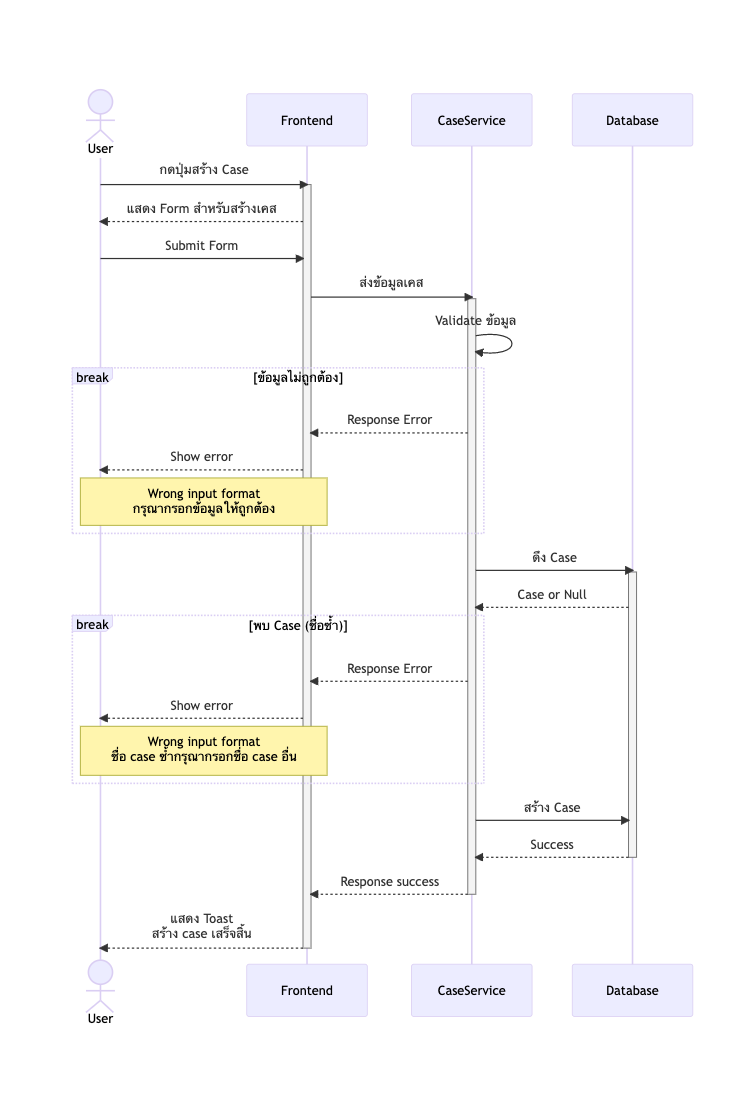
\includegraphics[width=15cm, trim={0 3cm 0 3cm},clip]{./assets/sequence-diagram/create-case.png}
        \caption{รูปแสดง Sequence diagram ของ Create case}\label{fig:sqCreateCase}
    \end{figure}

    \newpage
    \item \textbf{Archive case} \\
    เป็น sequence diagram ที่แสดงลำดับการทำงานของการเก็บคดีที่ได้จบไปเรียบร้อยแล้ว โดยมีรายละเอียดดังรูปที่ \ref{fig:sqArchiveCase} ดังนี้ 
    \begin{figure}[!ht]\centering
        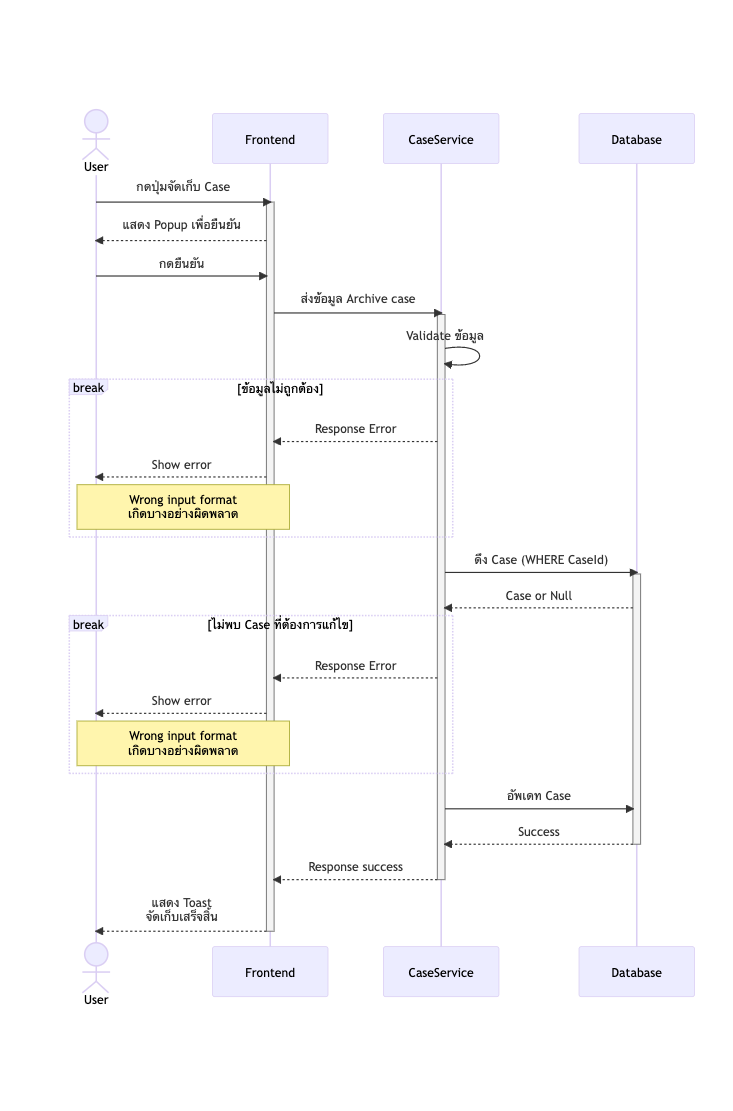
\includegraphics[width=15cm, trim={1cm 3cm 0.5cm 3cm},clip]{./assets/sequence-diagram/archive-case.png}
        \caption{รูปแสดง Sequence diagram ของ Archive case}\label{fig:sqArchiveCase}
    \end{figure}

    \newpage
    \item \textbf{Delete case} \\
    เป็น sequence diagram ที่แสดงลำดับการทำงานของการลบคดีที่ไม่ต้องการเก็บไว้ โดยมีรายละเอียดดังรูปที่ \ref{fig:sqDeleteCase} ดังนี้ 
    \begin{figure}[!ht]\centering
        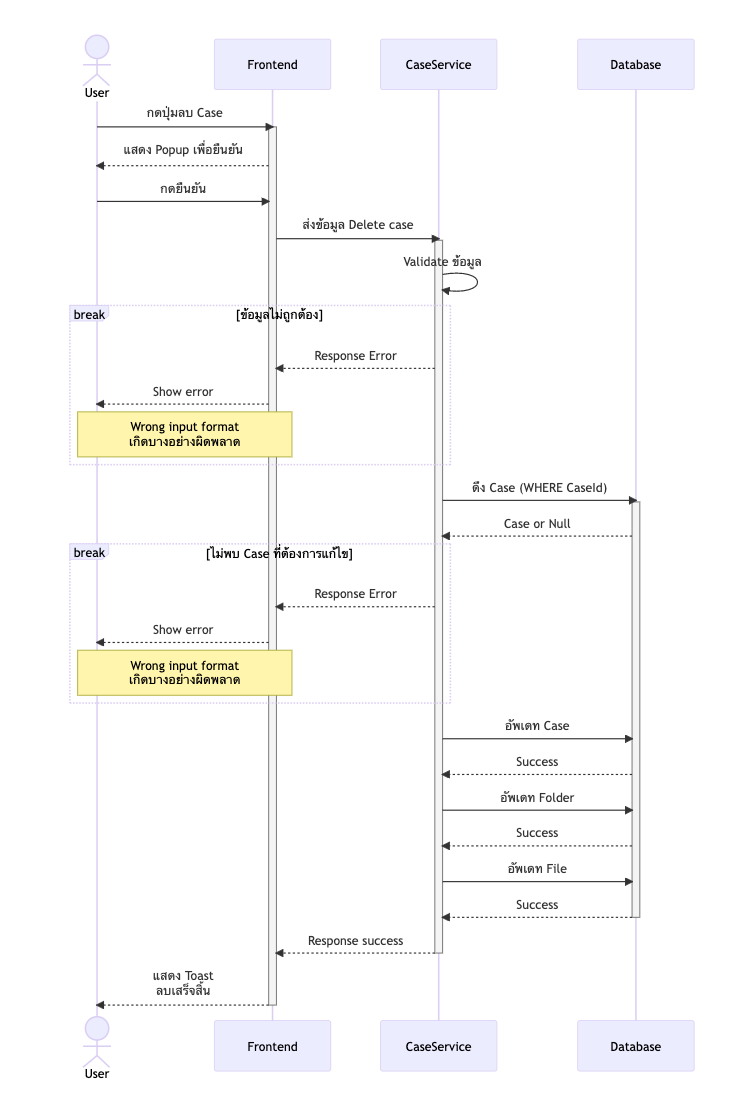
\includegraphics[width=14cm, trim={1.5cm 1cm 1 1cm},clip]{./assets/sequence-diagram/delete-case.png}
        \caption{รูปแสดง Sequence diagram ของ Delete case}\label{fig:sqDeleteCase}
    \end{figure}

    \newpage
    \item \textbf{Search file} \\
    เป็น sequence diagram ที่แสดงลำดับการทำงานของการค้นหาไฟล์ที่ต้องการ โดยมีรายละเอียดดังรูปที่ \ref{fig:sqSearchFile} ดังนี้
    \begin{figure}[!ht]\centering
        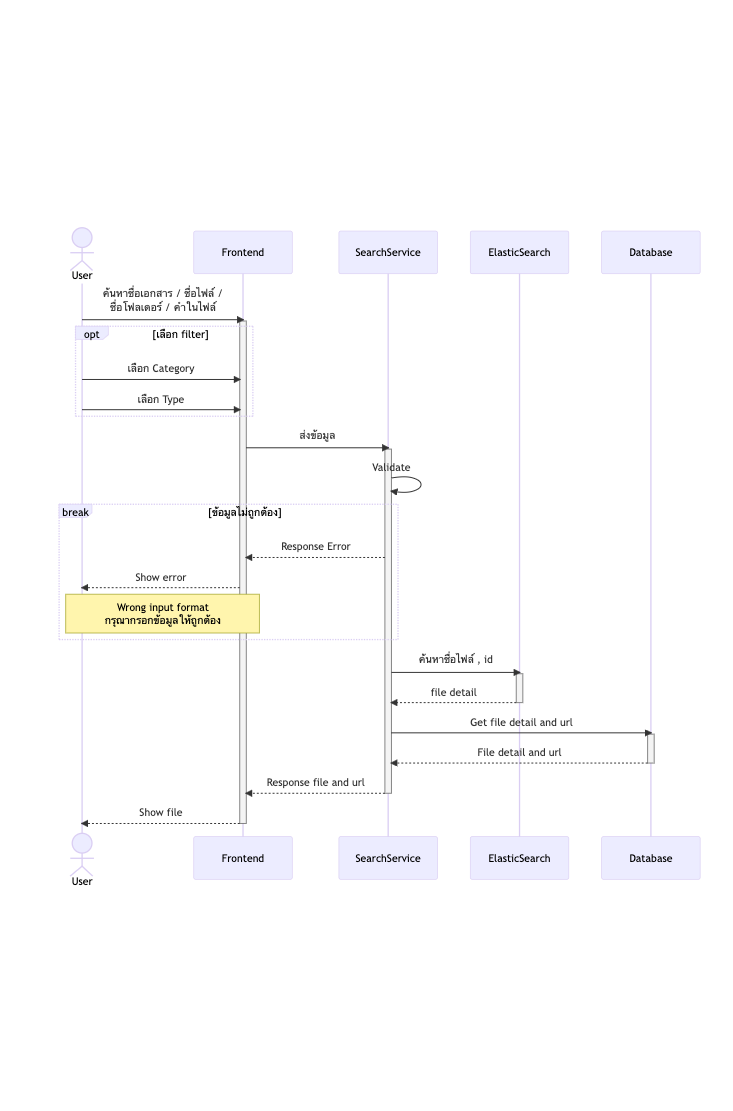
\includegraphics[width=15cm, trim={1cm 7.2cm 0.5cm 7.3cm},clip]{./assets/sequence-diagram/search-file.png}
        \caption{รูปแสดง Sequence diagram ของ Search file}\label{fig:sqSearchFile}
    \end{figure}

    \newpage
    \item \textbf{Upload file} \\
    เป็น sequence diagram ที่แสดงลำดับการทำงานของการอัพโหลดไฟล์เข้าสู่ระบบ โดยมีรายละเอียดดังรูปที่ \ref{fig:sqUploadFile} ดังนี้
    \begin{figure}[!ht]\centering
        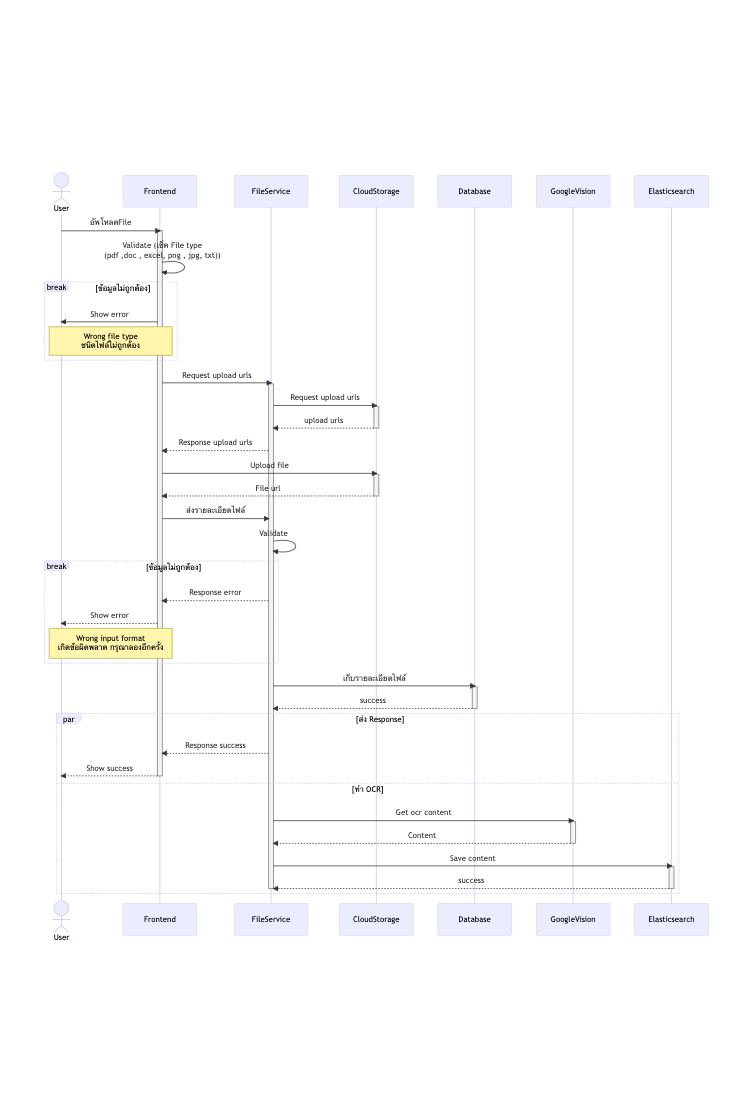
\includegraphics[width=15cm, trim={1cm 6cm 0.5cm 6cm},clip]{./assets/sequence-diagram/upload-file.png}
        \caption{รูปแสดง Sequence diagram ของ Upload file}\label{fig:sqUploadFile}
    \end{figure}


    \newpage
    \item \textbf{Create appointment} \\
    เป็น sequence diagram ที่แสดงลำดับการทำงานของการสร้างนัดหมายกับลูกความ โดยมีรายละเอียดดังรูปที่ \ref{fig:sqCreateEvent} ดังนี้
    \begin{figure}[!ht]\centering
        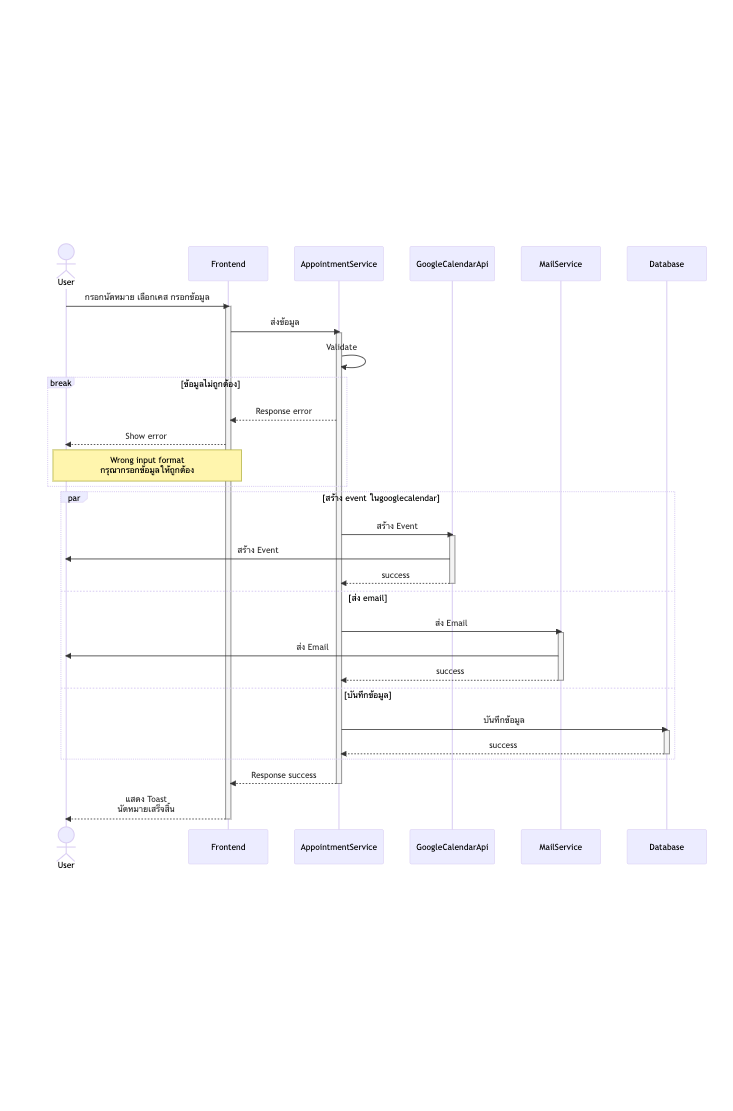
\includegraphics[width=15cm, trim={0 7cm 0 7cm},clip]{./assets/sequence-diagram/create-event.png}
        \caption{รูปแสดง Sequence diagram ของ Create appointment}\label{fig:sqCreateEvent}
    \end{figure}

    \newpage
    \item \textbf{Edit appointment} \\
    เป็น sequence diagram ที่แสดงลำดับการทำงานของการแก้ไขนัดหมายกับลูกความ โดยมีรายละเอียดดังรูปที่ \ref{fig:sqEditEvent} ดังนี้
    \begin{figure}[!ht]\centering
        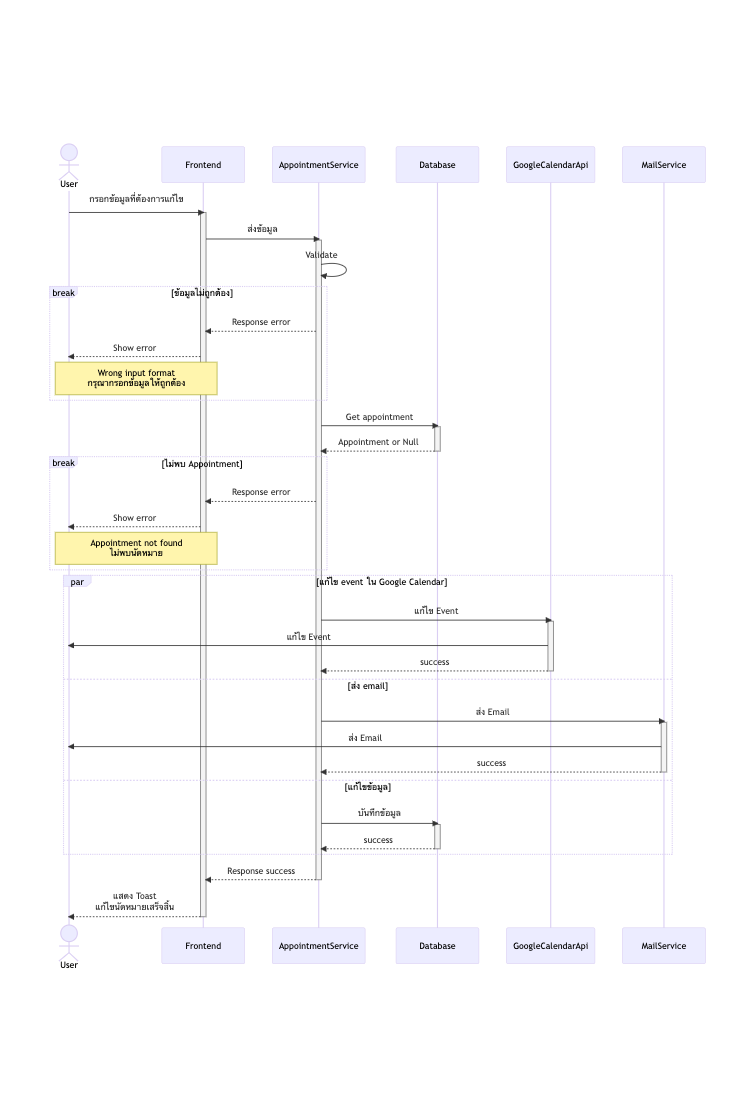
\includegraphics[width=15cm, trim={1cm 5cm 0.5cm 5cm},clip]{./assets/sequence-diagram/edit-event.png}
        \caption{รูปแสดง Sequence diagram ของ Edit appointment}\label{fig:sqEditEvent}
    \end{figure}

    \newpage
    \item \textbf{Create user} \\
    เป็น sequence diagram ที่แสดงลำดับการทำงานของการสร้างผู้ใช้งานใหม่ โดยมีรายละเอียดดังรูปที่ \ref{fig:sqCreateUser} ดังนี้
    \begin{figure}[!ht]\centering
        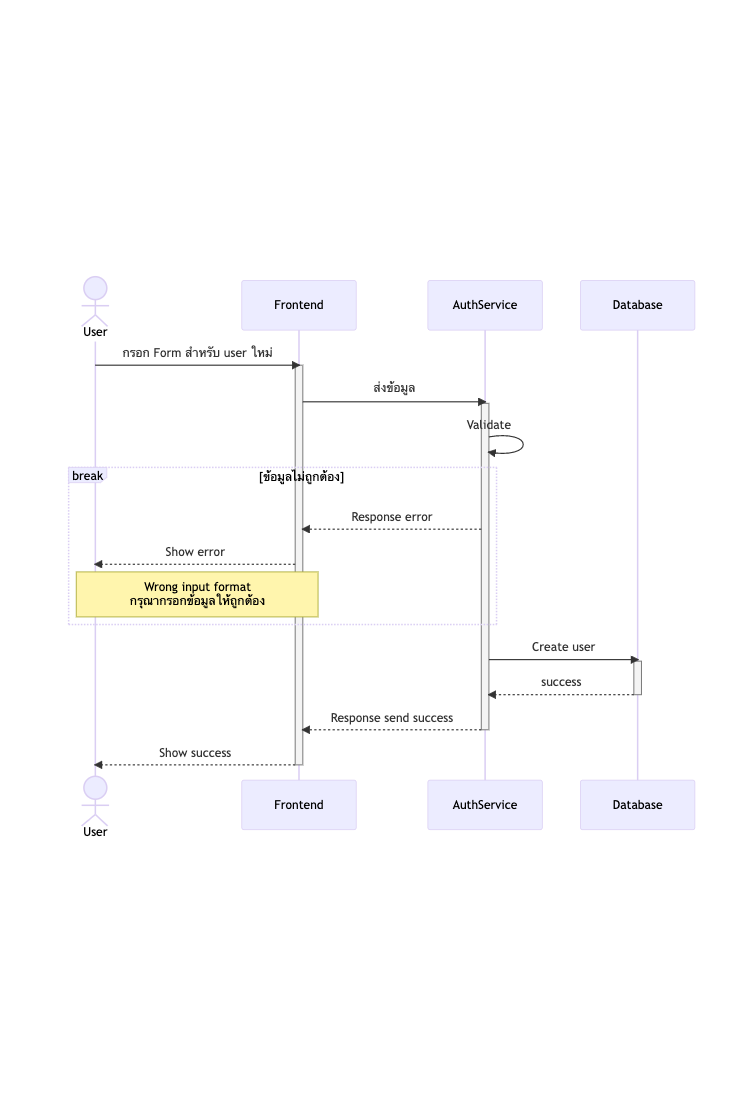
\includegraphics[width=15cm, trim={1cm 9cm 0.5cm 9cm},clip]{./assets/sequence-diagram/create-user.png}
        \caption{รูปแสดง Sequence diagram ของ Create user}\label{fig:sqCreateUser}
    \end{figure}

    \newpage
    \item \textbf{Edit profile} \\
    เป็น sequence diagram ที่แสดงลำดับการทำงานของการแก้ไขข้อมูลส่วนตัว โดยมีรายละเอียดดังรูปที่ \ref{fig:sqEditProfile} ดังนี้
    \begin{figure}[!ht]\centering
        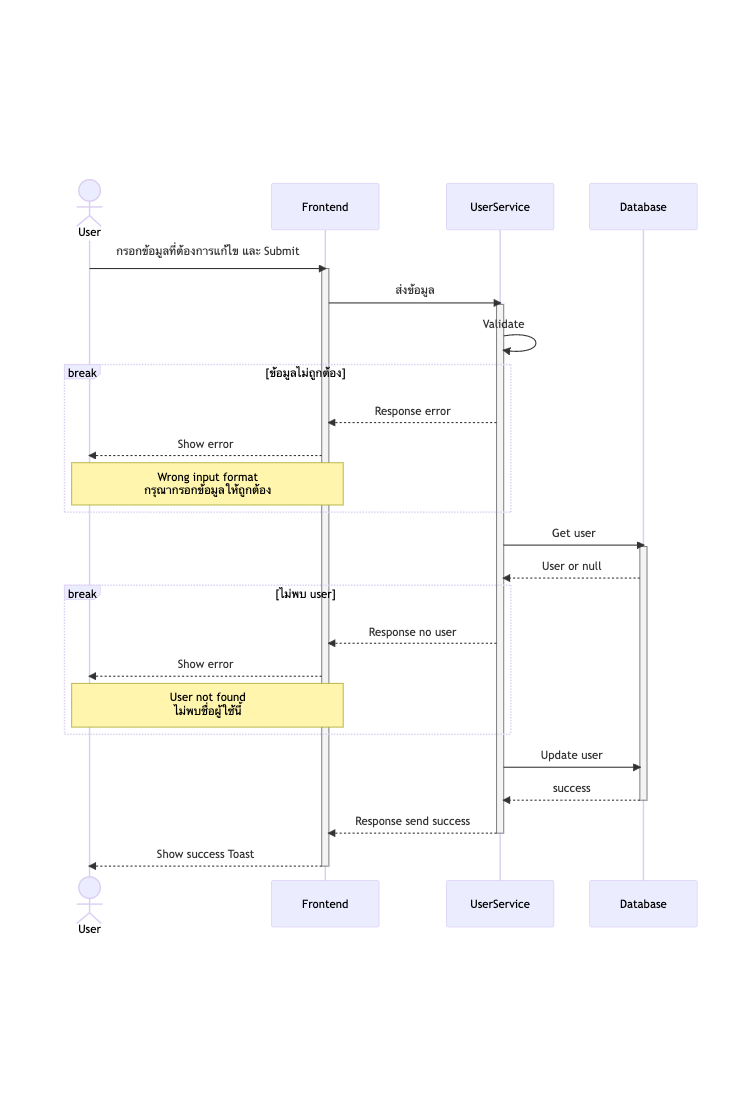
\includegraphics[width=15cm, trim={0 6cm 0 6cm},clip]{./assets/sequence-diagram/edit-profile.png}
        \caption{รูปแสดง Sequence diagram ของ Edit profile}\label{fig:sqEditProfile}
    \end{figure}

    \newpage
    \item \textbf{Login} \\
    เป็น sequence diagram ที่แสดงลำดับการทำงานของการเข้าสู่ระบบ โดยมีรายละเอียดดังรูปที่ \ref{fig:sqLogin} ดังนี้
    \begin{figure}[!ht]\centering
        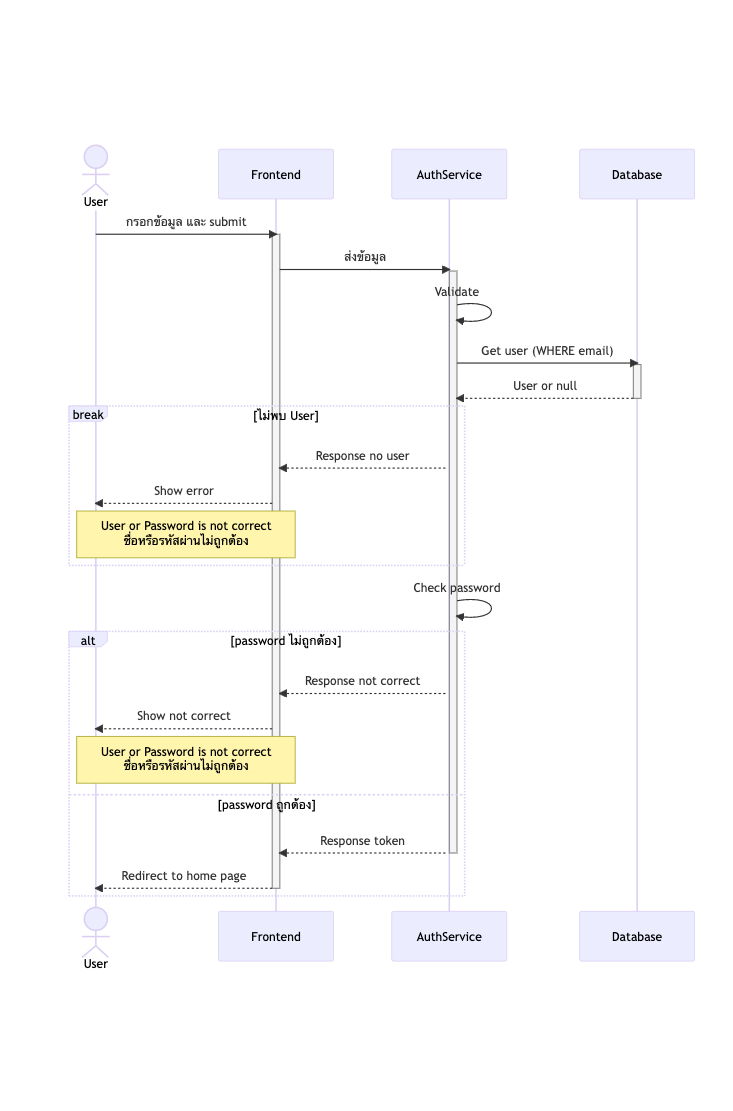
\includegraphics[width=15cm, trim={1cm 5cm 0.5cm 5cm},clip]{./assets/sequence-diagram/login.png}
        \caption{รูปแสดง Sequence diagram ของ Login}\label{fig:sqLogin}
    \end{figure}

    \newpage
    \item \textbf{Forget password} \\
    เป็น sequence diagram ที่แสดงลำดับการทำงานของการเปลี่ยนรหัสผ่าน โดยมีรายละเอียดดังรูปที่ \ref{fig:sqForgetPassword} ดังนี้
    \begin{figure}[!ht]\centering
        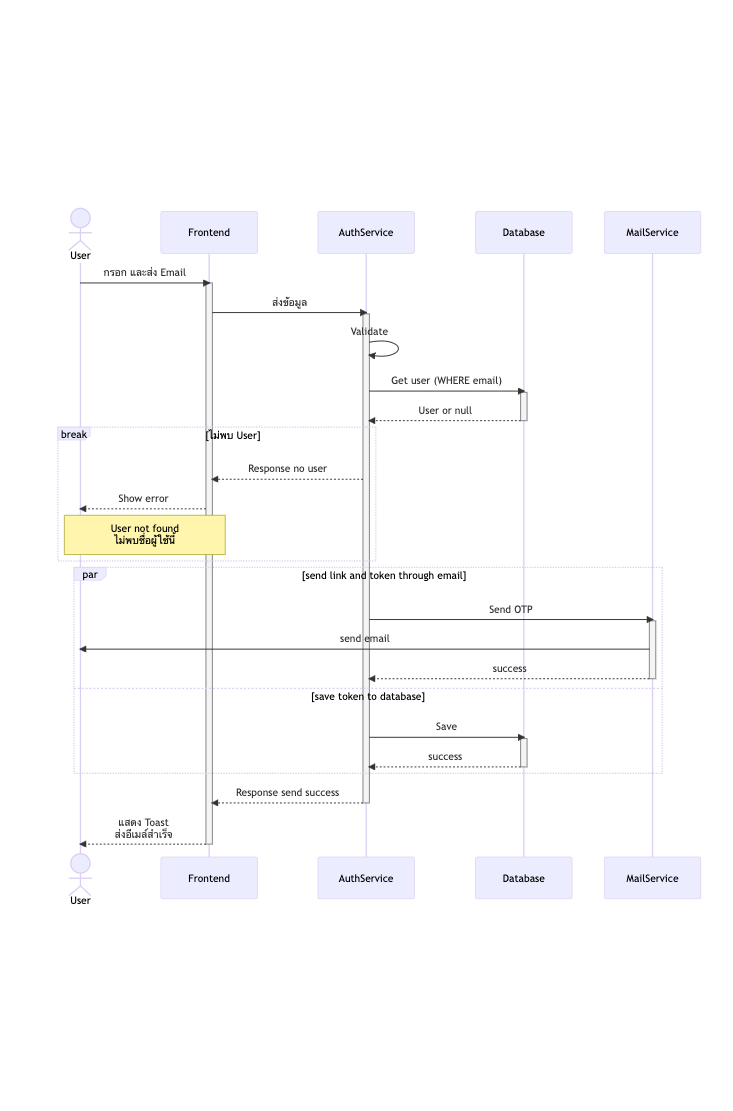
\includegraphics[width=15cm, trim={0 7cm 0 7cm},clip]{./assets/sequence-diagram/forget-password.png}
        \caption{รูปแสดง Sequence diagram ของ Forget password}\label{fig:sqForgetPassword}
    \end{figure}

    
    \newpage
    \item \textbf{Reset password} \\
    เป็น sequence diagram ที่แสดงลำดับการทำงานของการรีเซ็ตรหัสผ่าน โดยมีรายละเอียดดังรูปที่ \ref{fig:sqResetPassword} ดังนี้
    \begin{figure}[!ht]\centering
        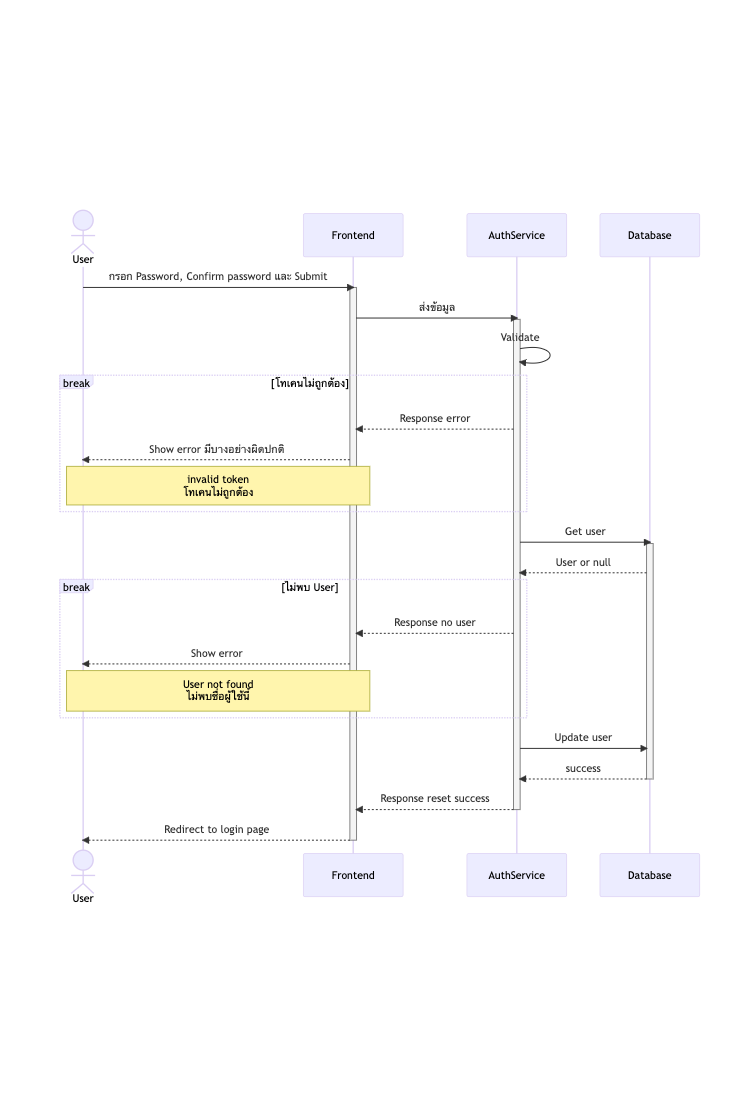
\includegraphics[width=15cm, trim={1cm 7cm 0.5cm 7cm},clip]{./assets/sequence-diagram/reset-password.png}
        \caption{รูปแสดง Sequence diagram ของ Reset password}\label{fig:sqResetPassword}
    \end{figure}

        
    \newpage
    \item \textbf{Change password}\\
    เป็น sequence diagram ที่แสดงลำดับการทำงานของการเปลี่ยนรหัสผ่าน โดยมีรายละเอียดดังรูปที่ \ref{fig:sqChangePassword} ดังนี้
    \begin{figure}[!ht]\centering
        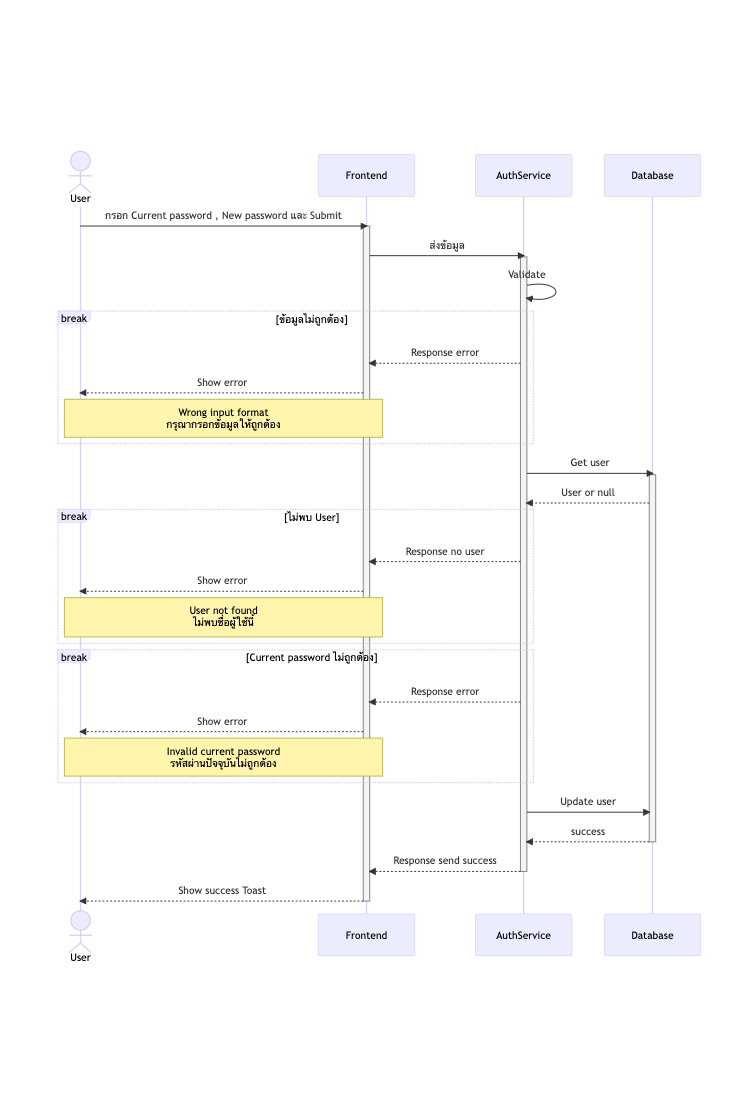
\includegraphics[width=15cm, trim={1cm 5cm 0.5cm 5cm},clip]{./assets/sequence-diagram/change-password.png}
        \caption{รูปแสดง Sequence diagram ของ Change password}\label{fig:sqChangePassword}
    \end{figure}

    
\end{itemize}
\newpage
\section{User Interface Design}
\subsection{Base Component}
\hspace*{1cm} เป็นส่วนประกอบหลักที่ถูกใช้ในหน้าต่าง ๆ โดยจะมีทั้ง ตารางแสดงโฟล์เดอร์ ไฟล์ และช่องค้นหาข้อมูลรวมไปถึงแสดงการใช้ฟังก์ชันต่าง ๆ ดังนี้
\begin{itemize}
  \item \textbf{Case folder component} \\
\hspace*{1cm} เป็นส่วนประกอบหลัก ที่ประกอบไปด้วยตารางแสดงข้อมูลโฟล์เดอร์ และแสดงการใช้ฟังก์ชันต่าง ๆ ดังรูป \ref{fig:folder-component} - \ref{fig:delete-folder} ดังนี้
\begin{figure}[!h]\centering
  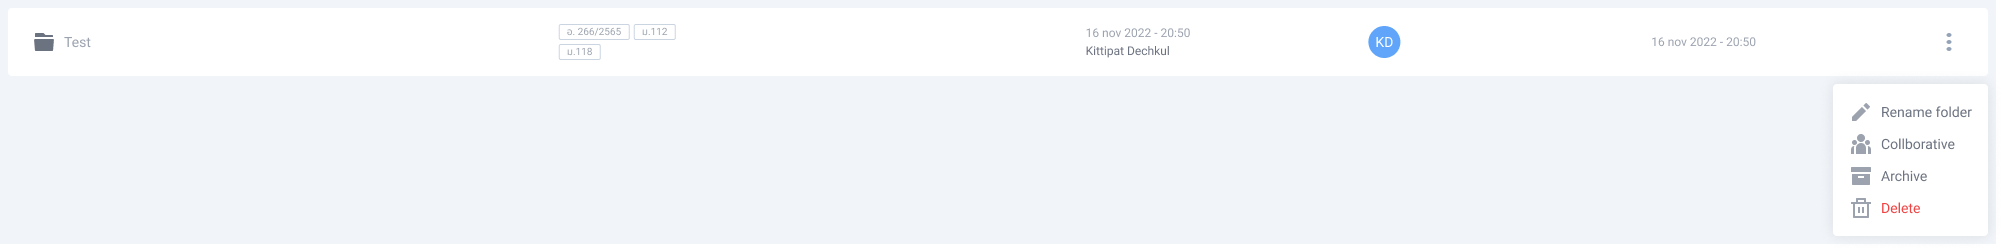
\includegraphics[width=13cm]{./assets/userinterface/folder-component.png}
  \caption{รูปแสดงการออกแบบตารางแสดงข้อมูลโฟล์เดอร์}\label{fig:folder-component}
\end{figure}

\begin{figure}[!h]\centering
  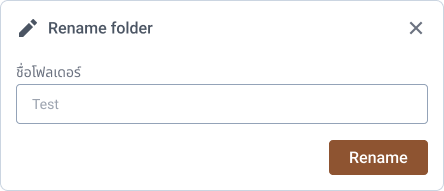
\includegraphics[width=8cm]{./assets/userinterface/rename-folder.png}
  \caption{รูปแสดงการออกแบบหน้าแก้ไขชื่อโฟล์เดอร์}\label{fig:rename-folder}
\end{figure}

\begin{figure}[!h]\centering
  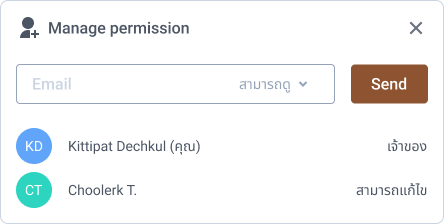
\includegraphics[width=8cm]{./assets/userinterface/manage-folder-permission.png}
  \caption{รูปแสดงการออกแบบหน้าแก้ไขสิทธ์การเข้าถึงโฟล์เดอร์}\label{fig:manage-folder-permission}
\end{figure}

\begin{figure}[!h]\centering
  
\includegraphics[width=8cm]{./assets/userinterface/archive-folder.png}
  \caption{รูปแสดงการออกแบบหน้าจัดเก็บโฟล์เดอร์}\label{fig:archive-folder}
\end{figure}

\begin{figure}[!h]\centering
  
\includegraphics[width=8cm]{./assets/userinterface/delete-folder.png}
  \caption{รูปแสดงการออกแบบหน้าลบโฟล์เดอร์}\label{fig:delete-folder}
\end{figure}

  \item \textbf{File component} \\
\hspace*{1cm} เป็นส่วนประกอบหลัก ที่ประกอบไปด้วยตารางแสดงข้อมูลไฟล์ และแสดงการใช้ฟังก์ชันต่าง ๆ ดังรูป \ref{fig:file-component} - \ref{fig:delete-file} ดังนี้

\begin{figure}[!h]\centering
  
\includegraphics[width=13cm]{./assets/userinterface/file-component.png}
  \caption{รูปแสดงการออกแบบตารางแสดงข้อมูลไฟล์}\label{fig:file-component}
\end{figure}

\begin{figure}[!h]\centering
  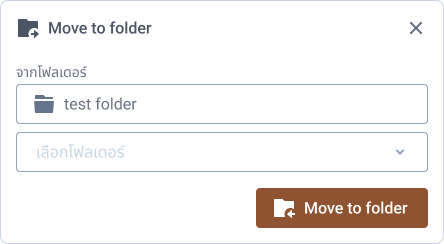
\includegraphics[width=8cm]{./assets/userinterface/move-to-folder.png}
  \caption{รูปแสดงการออกแบบหน้าย้านที่อยู่ไฟล์}\label{fig:move-to-folder}
\end{figure}

\begin{figure}[!h]\centering
  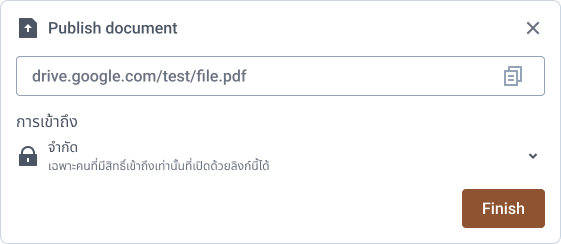
\includegraphics[width=8cm]{./assets/userinterface/publish-document.png}
  \caption{รูปแสดงการออกแบบหน้าเผยแพร่ไฟล์}\label{fig:publish-document}
\end{figure}

\begin{figure}[!h]\centering
  
\includegraphics[width=8cm]{./assets/userinterface/delete-file.png}
  \caption{รูปแสดงการออกแบบหน้าลบไฟล์}\label{fig:delete-file}
\end{figure}
\newpage
  \item \textbf{Search component} \\
\hspace*{1cm} เป็นส่วนประกอบหลัก ที่ประกอบไปด้วยช่องค้นหาข้อมูล และการใช้ฟังก์ชั่นกรองข้อมูล ดังรูป \ref{fig:search-filter} ดังนี้

\begin{figure}[!h]\centering
  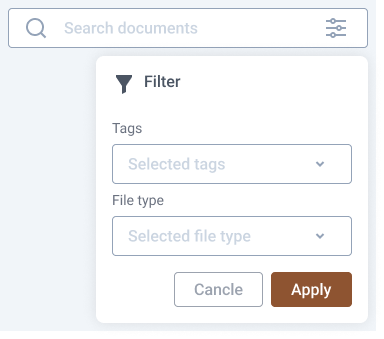
\includegraphics[width=8cm]{./assets/userinterface/search-filter.png}
  \caption{รูปแสดงการออกแบบหน้าค้นหาเอกสาร}\label{fig:search-filter}
\end{figure}

\end{itemize}
\newpage

\subsection{Landing Page}
\hspace*{1cm} เป็นหน้าแรกที่จะแสดงข้อมูลในรูปแบบแผนที่หรือแผนภูมิรูปต่าง ๆ โดยจะเป็นข้อมูลเกี่ยวกับกฎหมายหรือคดีต่าง ๆ ที่มีความน่าสนใจ ดังรูป \ref{fig:landing-page} ดังนี้
\begin{figure}[!h]\centering
  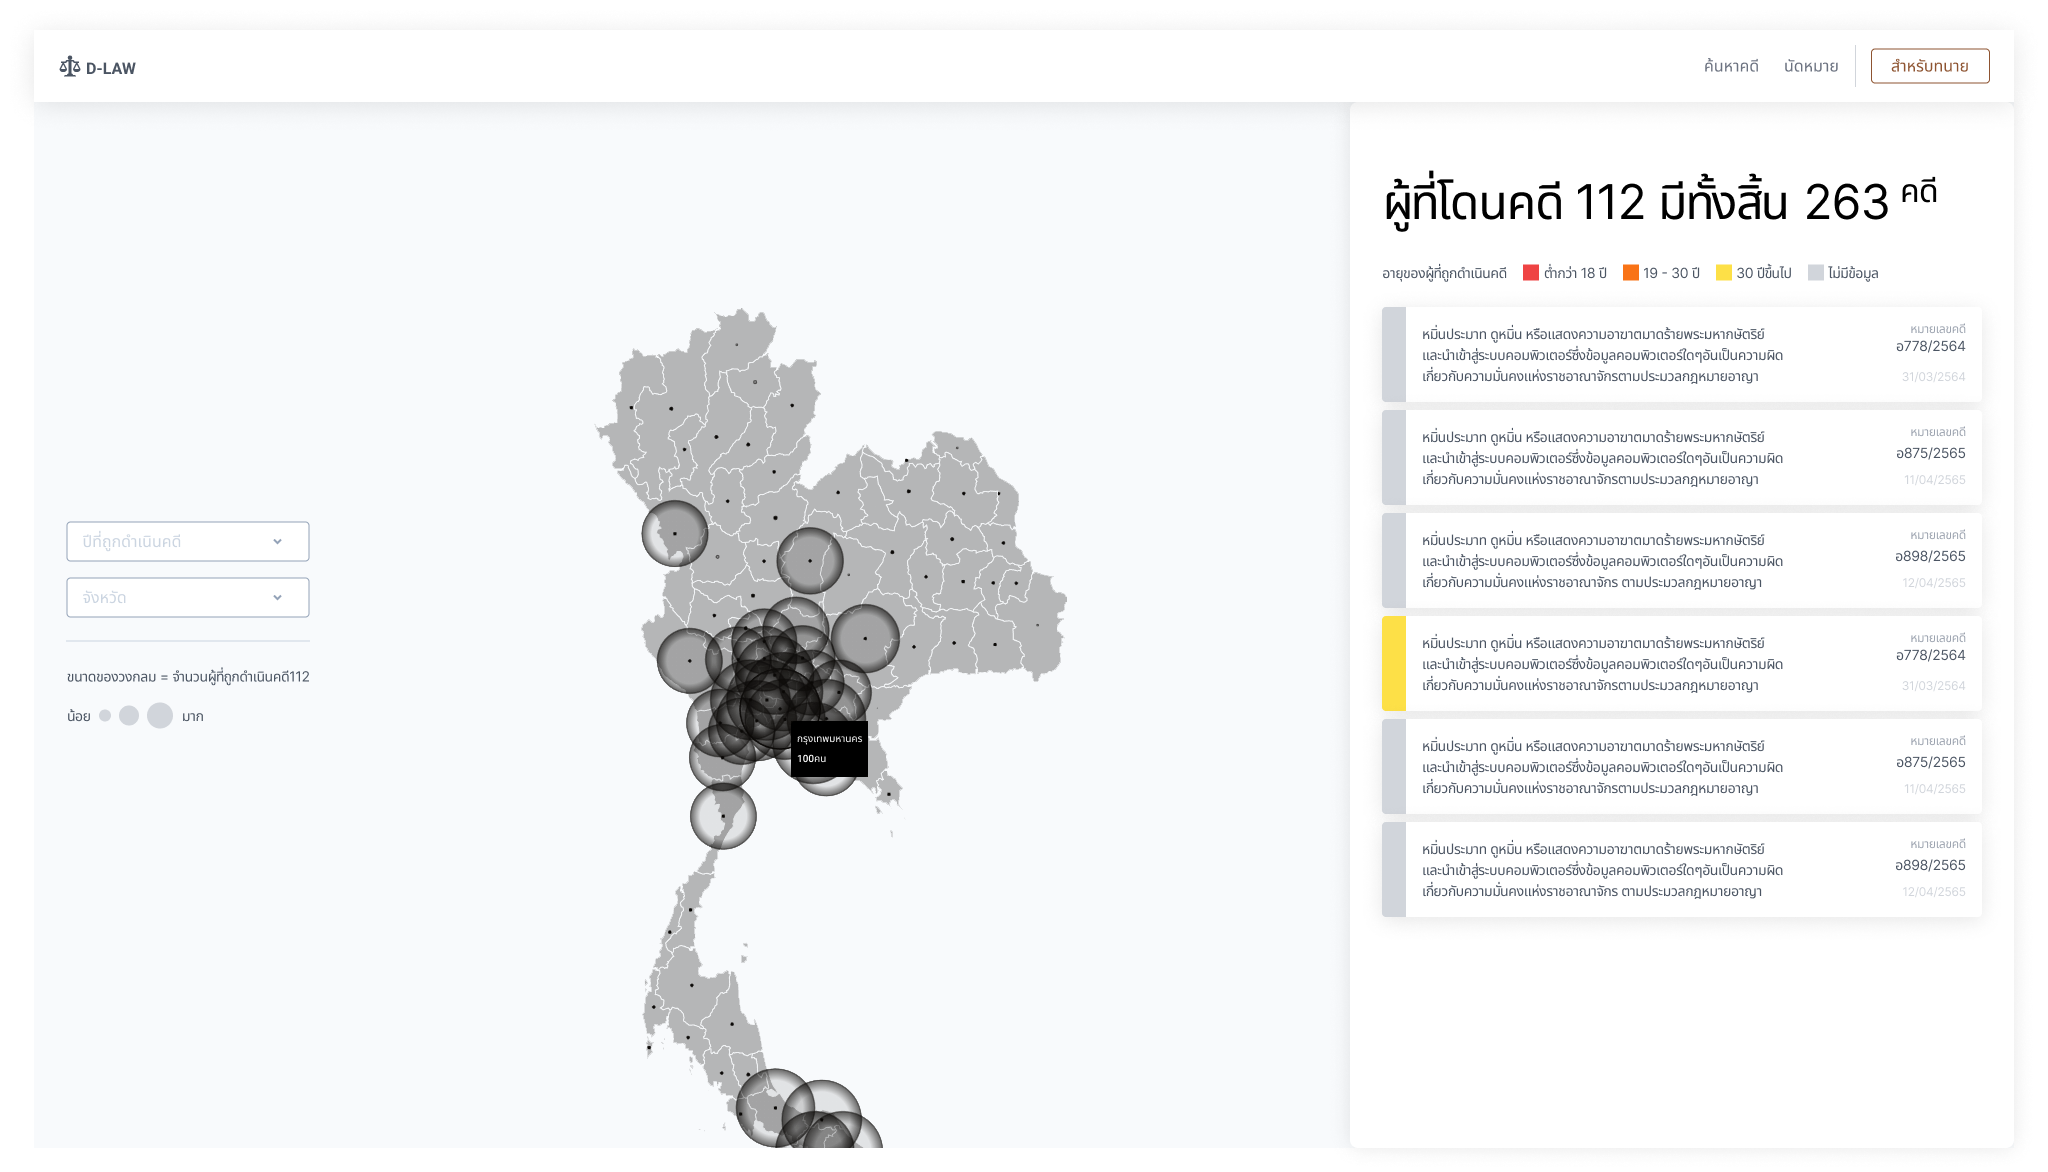
\includegraphics[width=13cm]{./assets/userinterface/landing-page.png}
  \caption{รูปแสดงการออกแบบหน้าแรกของเว็บไซต์}\label{fig:landing-page}
\end{figure}

\subsection{Search case Page}
\hspace*{1cm} เป็นหน้าที่จะใช้ค้นหาคดีต่าง ๆ โดยใช้หมายเลขคดีดำหรือหมายเลขคดีแดง ซึ่งจะสามารถแสดงรายระเอียดของคดีที่ต้องการค้นหาได้ ดังรูป \ref{fig:search-case} ดังนี้ 
\begin{figure}[!h]\centering
  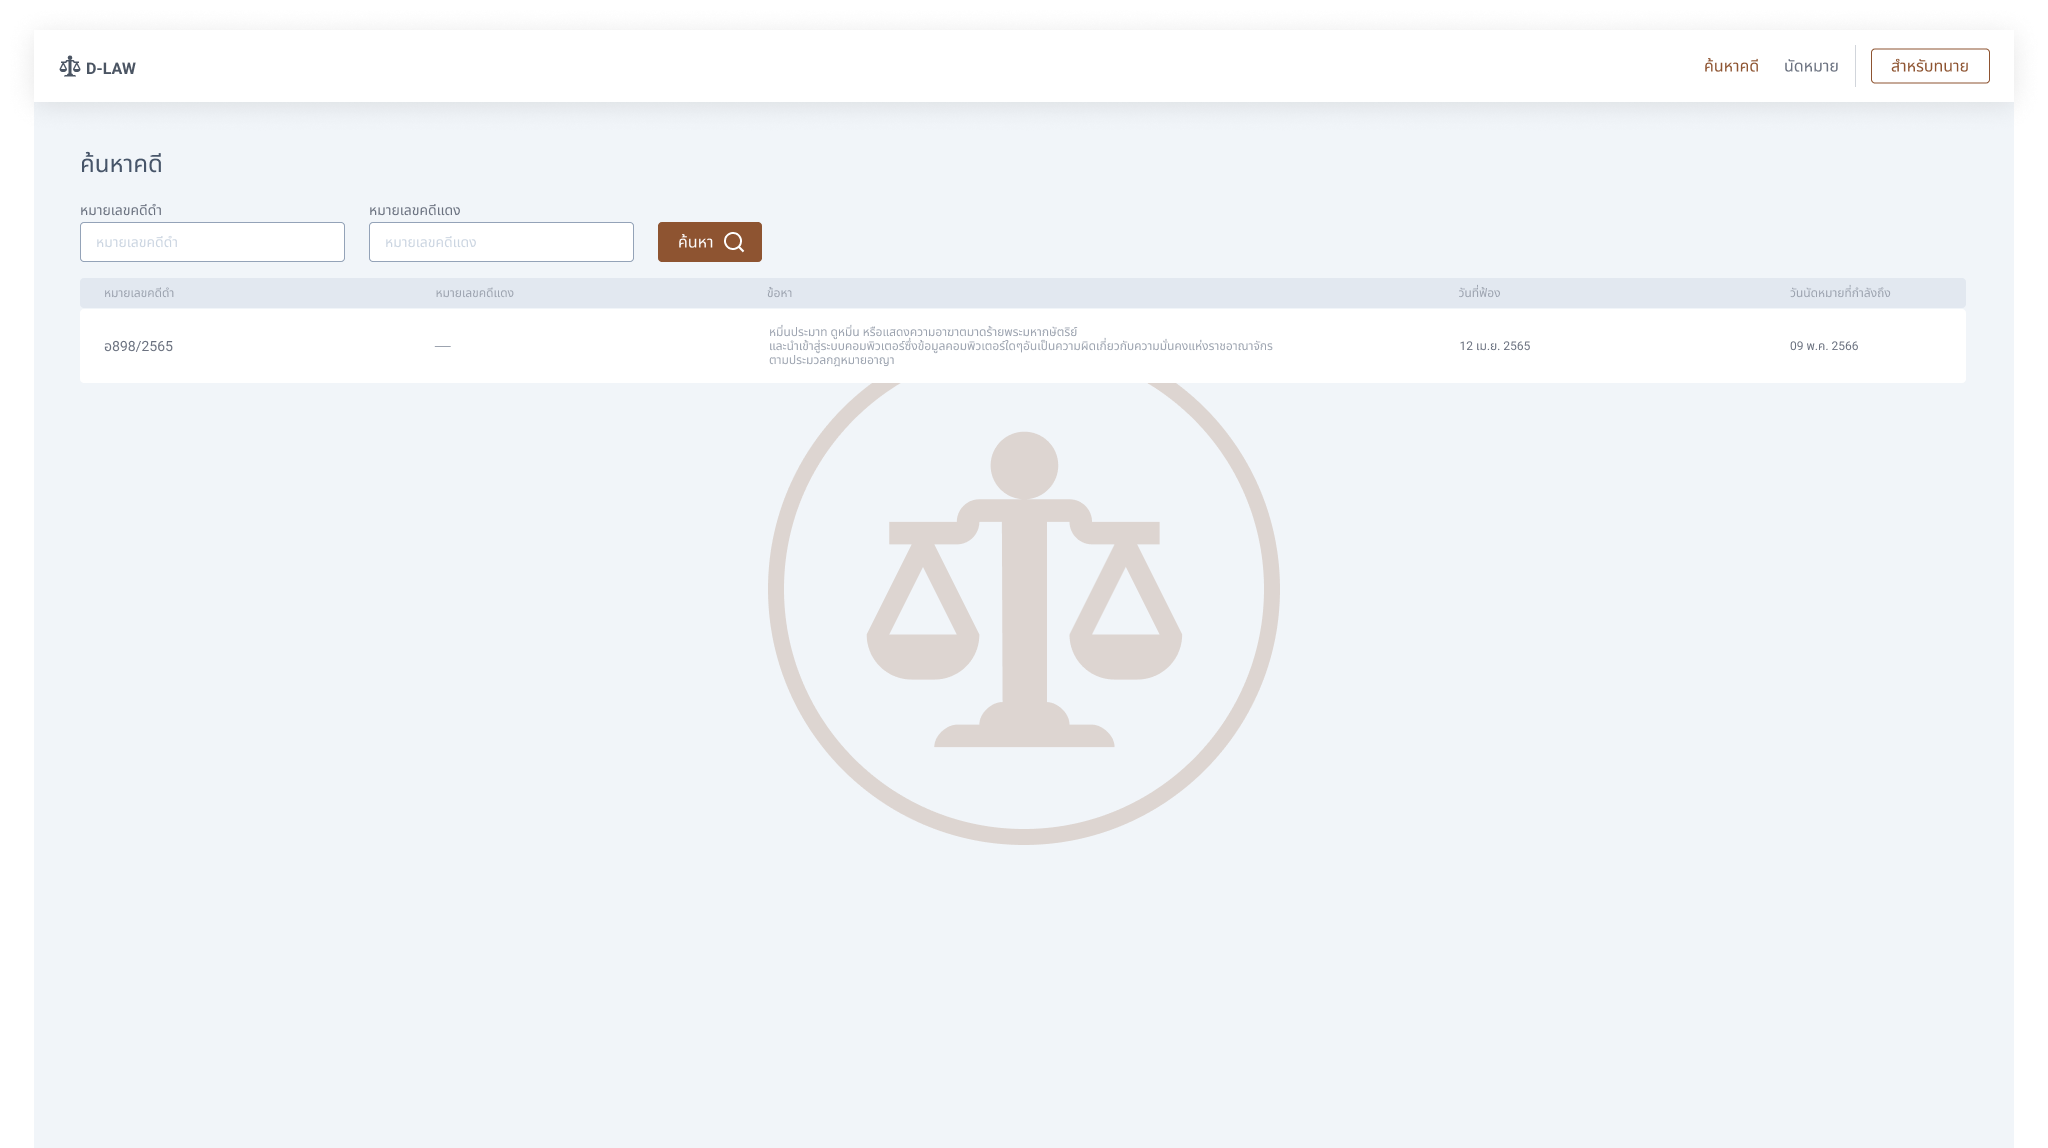
\includegraphics[width=13cm]{./assets/userinterface/search-case.png}
  \caption{รูปแสดงการออกแบบหน้าค้นหาข้อมูลคดี}\label{fig:search-case}
\end{figure}

\newpage
\subsection{Public appointment Page}
\hspace*{1cm} เป็นหน้าที่แสดงข้อมูลการนัดหมาย ที่ถูกเผยแพร่ให้คนทั่วไปสามารถดูข้อมูล และดาวน์โหลดเอกสารคดีได้ ดังรูป \ref{fig:appoinmtment-page} ดังนี้ 
\begin{figure}[!h]\centering
  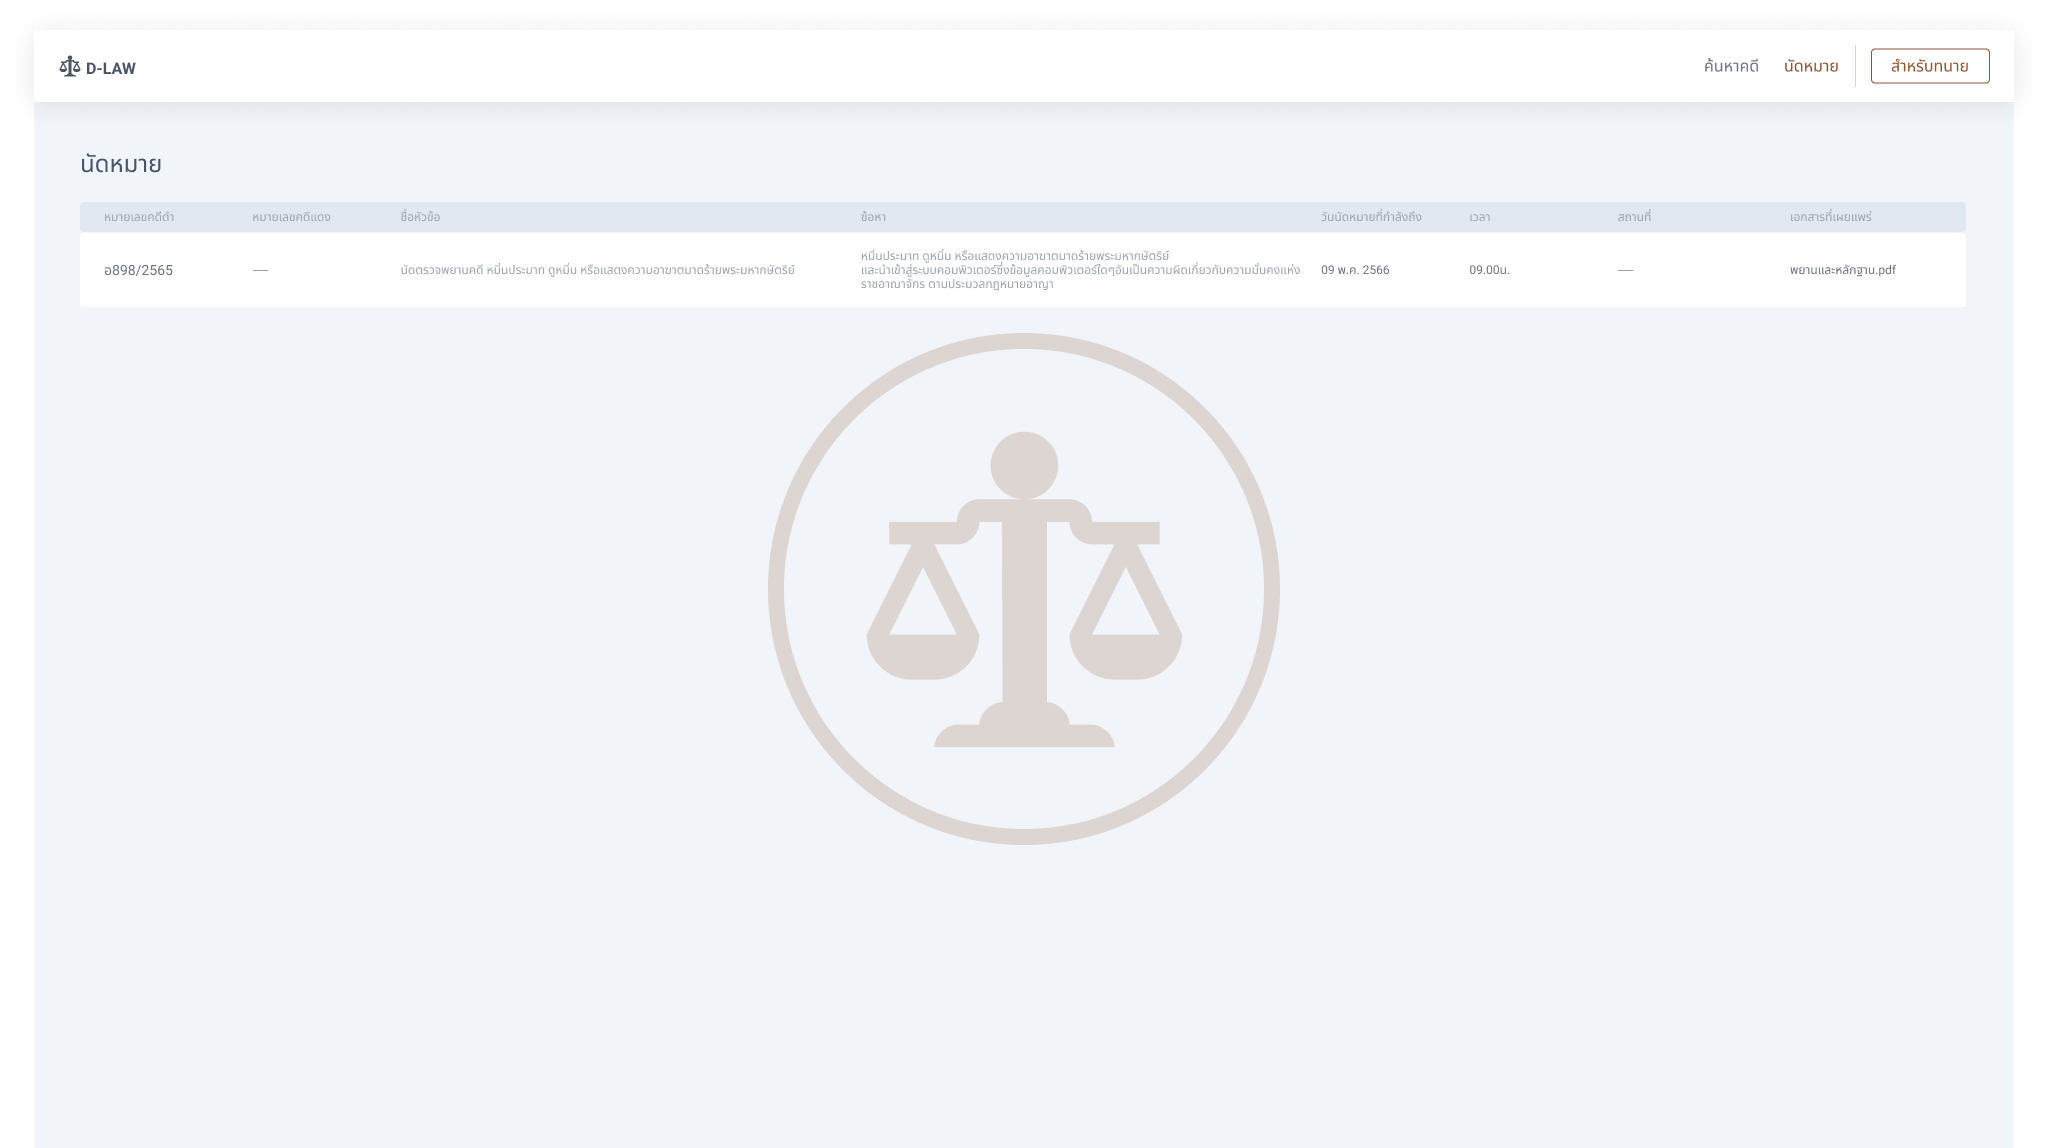
\includegraphics[width=13cm]{./assets/userinterface/appointment-public.png}
  \caption{รูปแสดงการออกแบบหน้าแสดงข้อมูลนัดหมายและเอกสาร}\label{fig:appoinmtment-page}
\end{figure}

\subsection{Login Page}
\hspace*{1cm} คือหน้าสำหรับการเข้าสู่ระบบ Document management system for lawyer โดยจะประกอบไปด้วยช่องกรอกอีเมล และพลาสเวิร์ด ดังรูป \ref{fig:login-page} ดังนี้
\begin{figure}[!h]\centering
  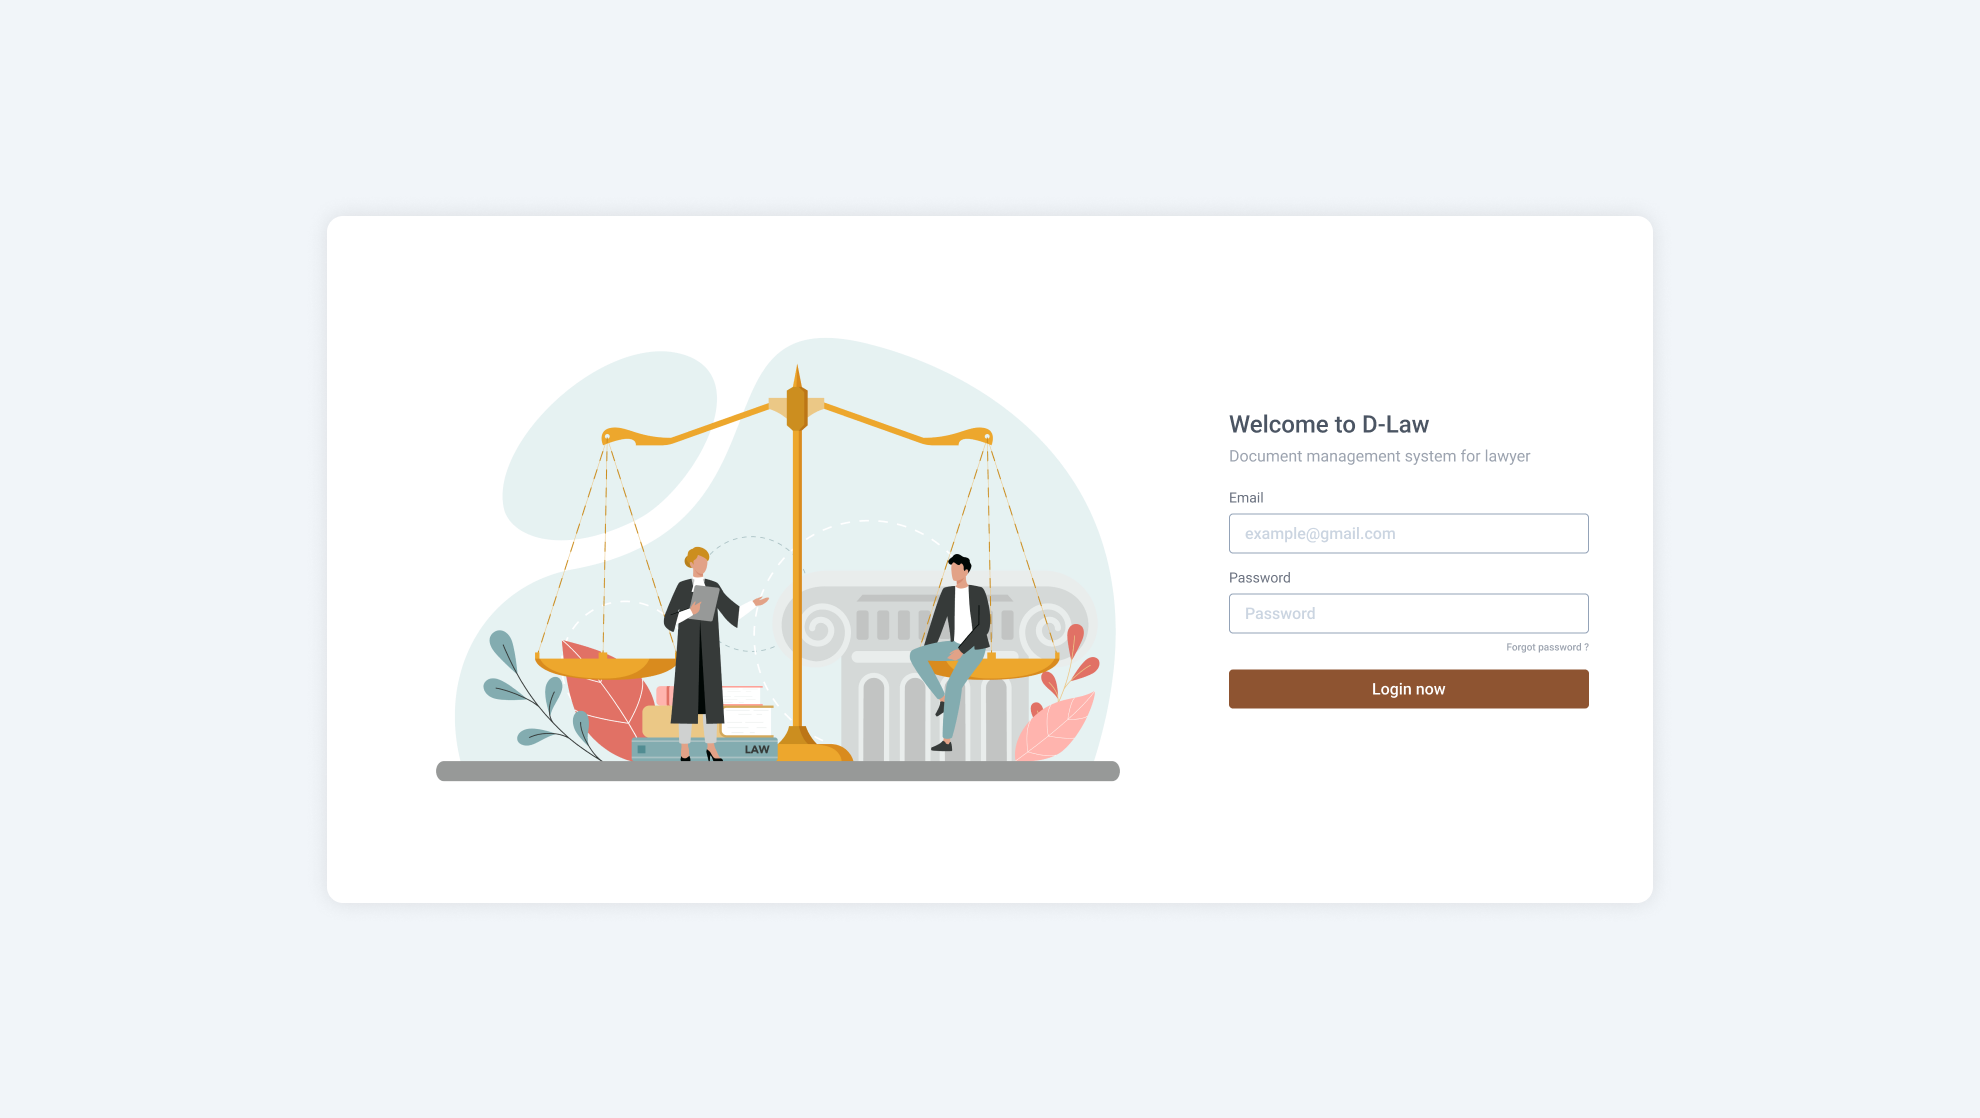
\includegraphics[width=13cm]{./assets/userinterface/login-page.png}
  \caption{รูปแสดงการออกแบบหน้าเข้าสู่ระบบ}\label{fig:login-page}
\end{figure}

\newpage
\subsection{Workspace Page}
\hspace*{1cm} หลังจากที่เข้าสู่ระบบมาจะเข้ามาสู่หน้าแสดงโฟล์เดอร์ และไฟล์ที่ถูกเรียกใช้บ่อย ๆ อีกทั้งยังสามารถกรองไฟล์ตามแท๊กได้ ดังรูป  \ref{fig:workspace-page} - \ref{fig:workspace-tags-filter} ดังนี้
\begin{figure}[!h]\centering
  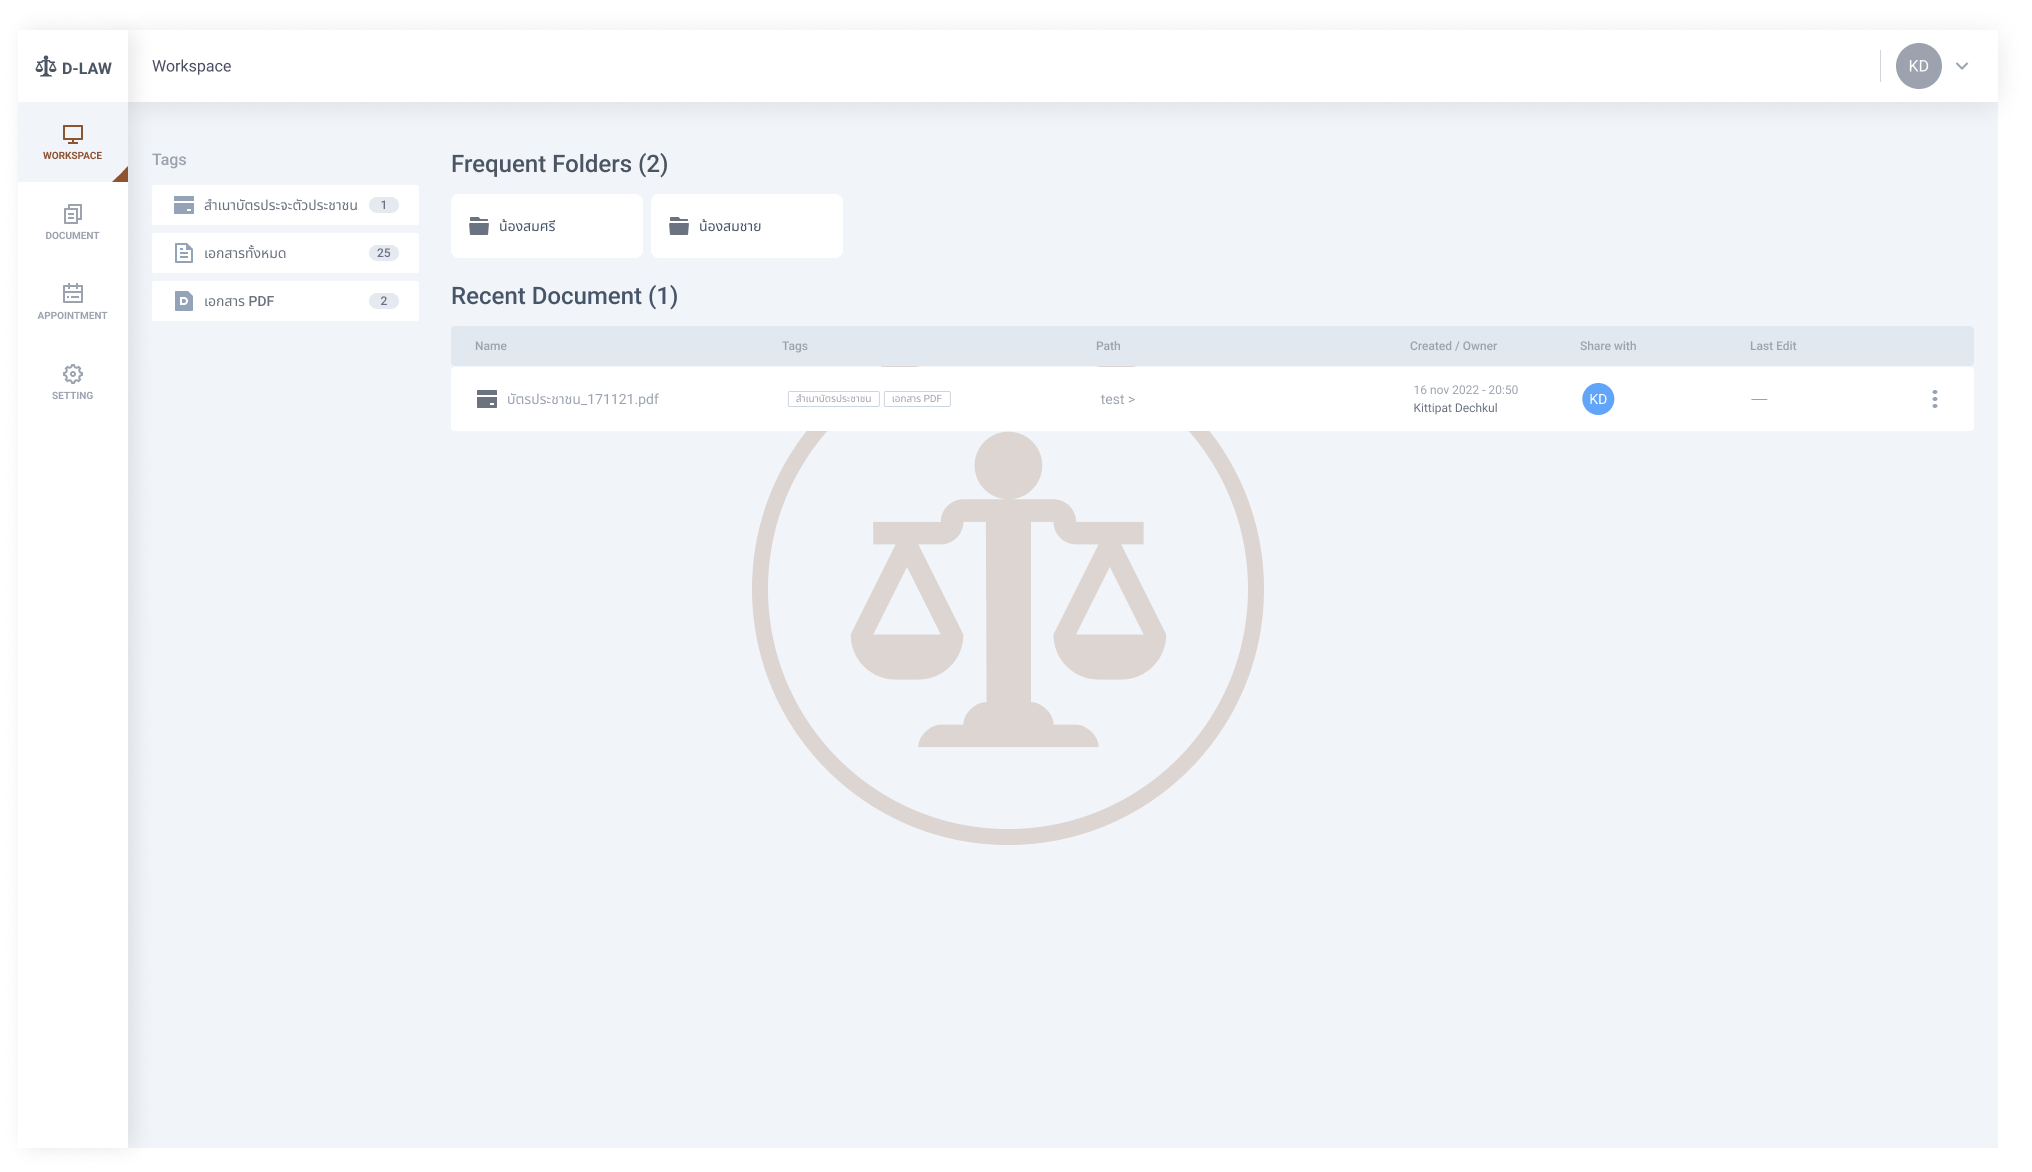
\includegraphics[width=13cm]{./assets/userinterface/workshop-page.png}
  \caption{รูปแสดงการออกแบบหน้าเข้าสู่ระบบ}\label{fig:workspace-page}
\end{figure}

\begin{figure}[!h]\centering
  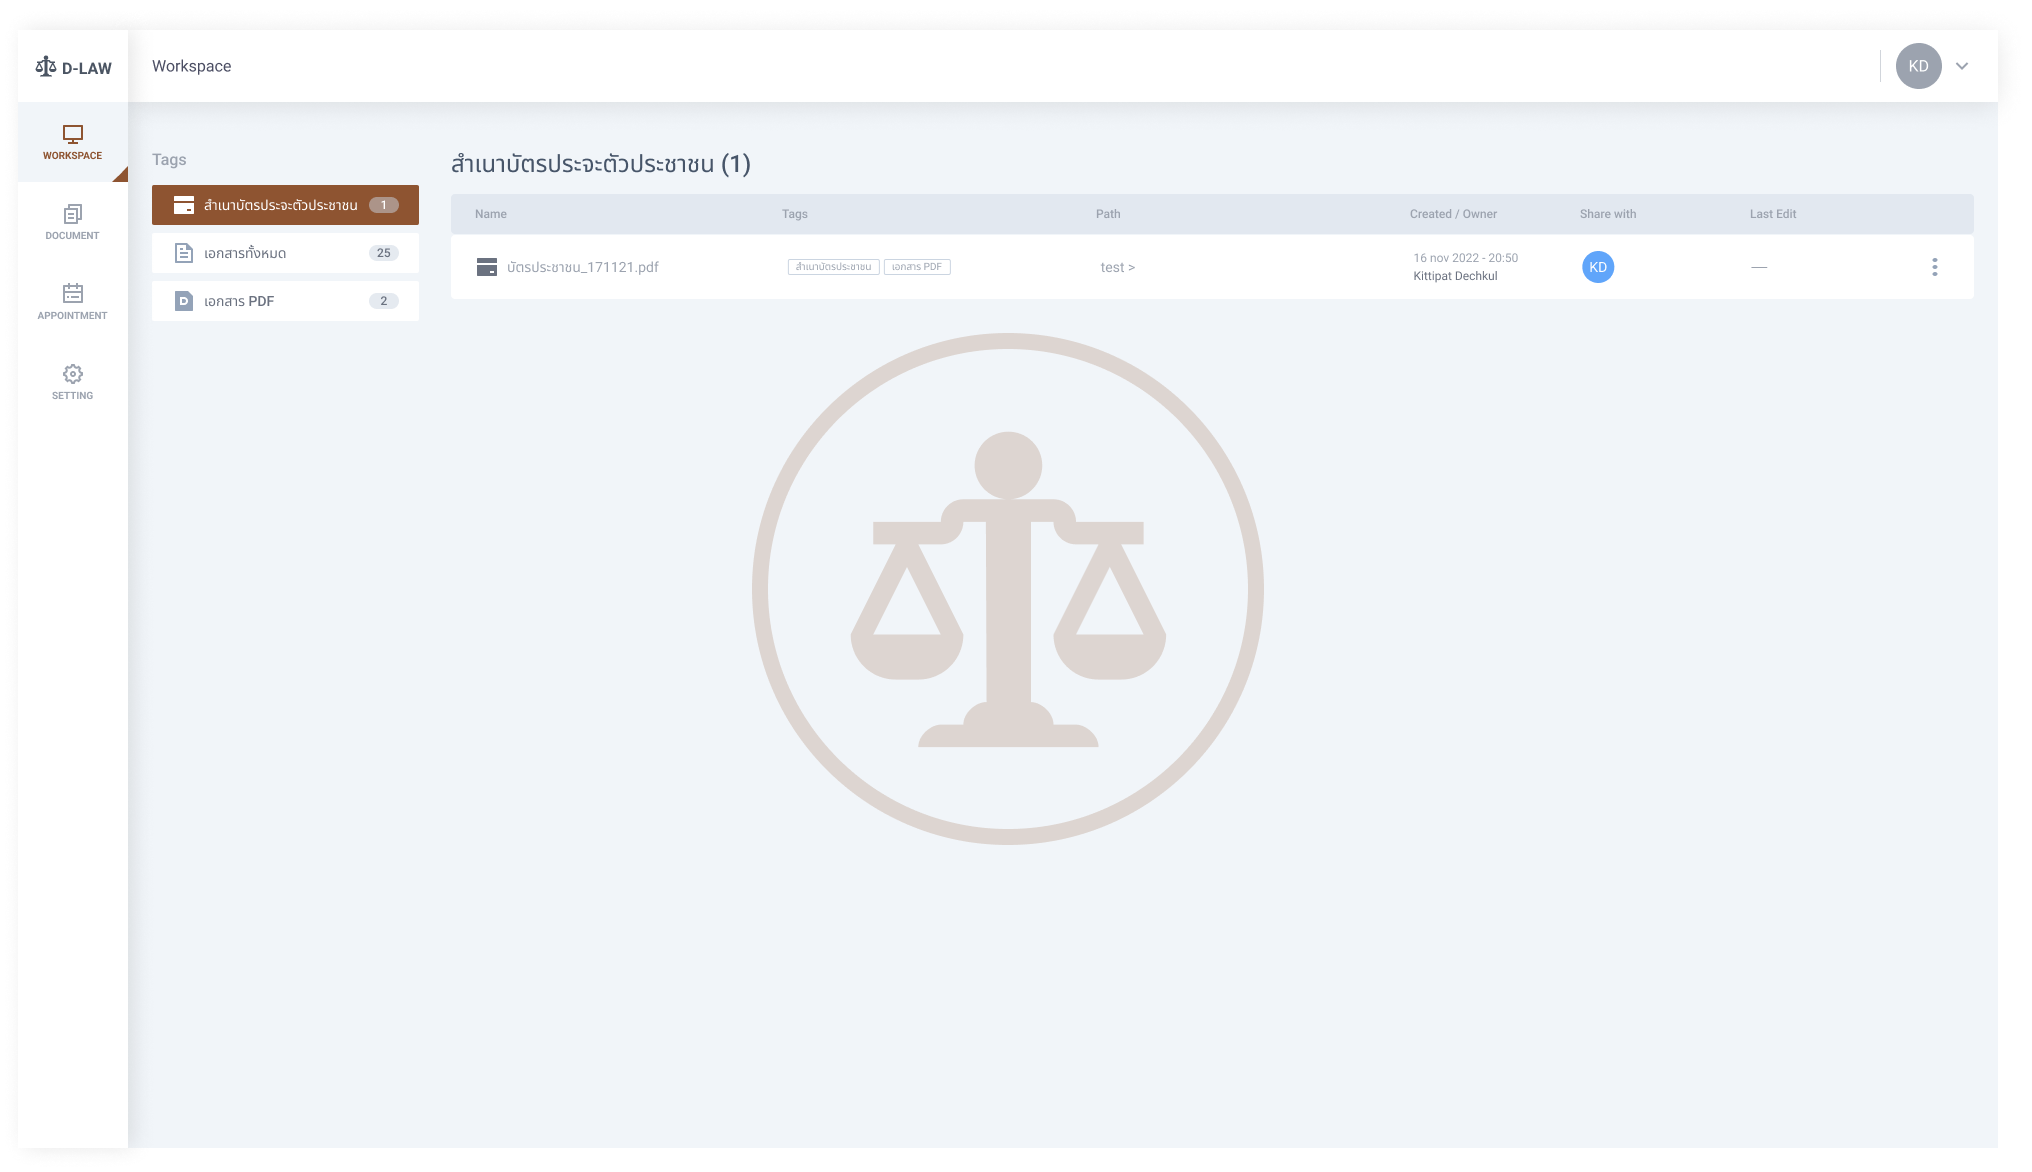
\includegraphics[width=13cm]{./assets/userinterface/workshop-tags-filter.png}
  \caption{รูปแสดงการออกแบบการกรองไฟล์ตามแท๊ก}\label{fig:workspace-tags-filter}
\end{figure}

\newpage
\subsection{Doucment Page}
\hspace*{1cm} เป็นหน้าที่จะแสดง โฟล์เดอร์เคสและไฟล์เอกสารต่าง ๆ ซื่อจะสามารถสร้าง อัพโหลด เผยแพร่ และสามารถใช้ฟังก์ชันอื่น ๆ ได้ ดังรูป \ref{fig:case-folder} - \ref{fig:activity-logs} ดังนี้
\begin{figure}[!h]\centering
  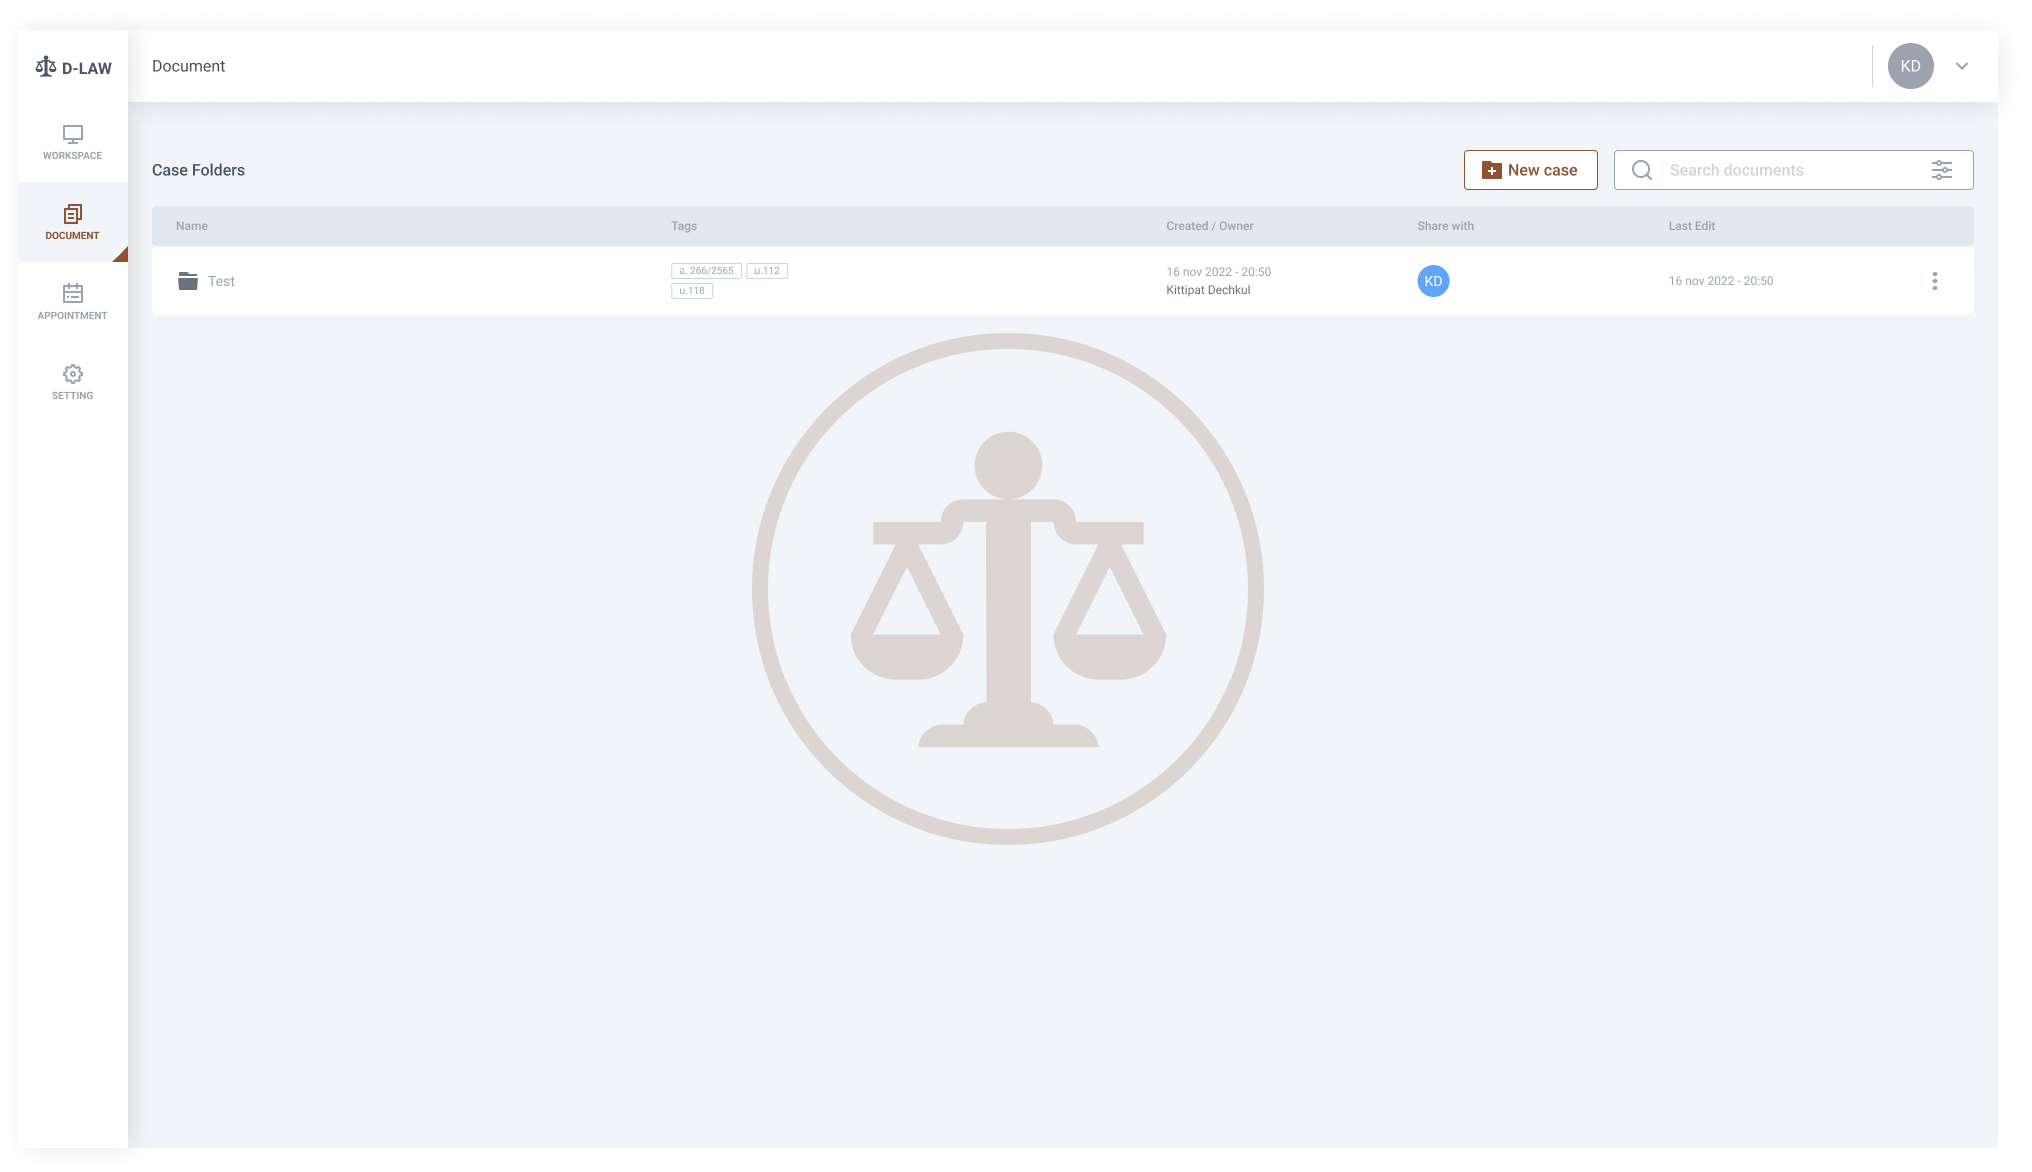
\includegraphics[width=13cm]{./assets/userinterface/case-folder.png}
  \caption{รูปแสดงการออกแบบหน้าตารางแสดงเคสต่าง ๆ}\label{fig:case-folder}
\end{figure}

\begin{figure}[!h]\centering
  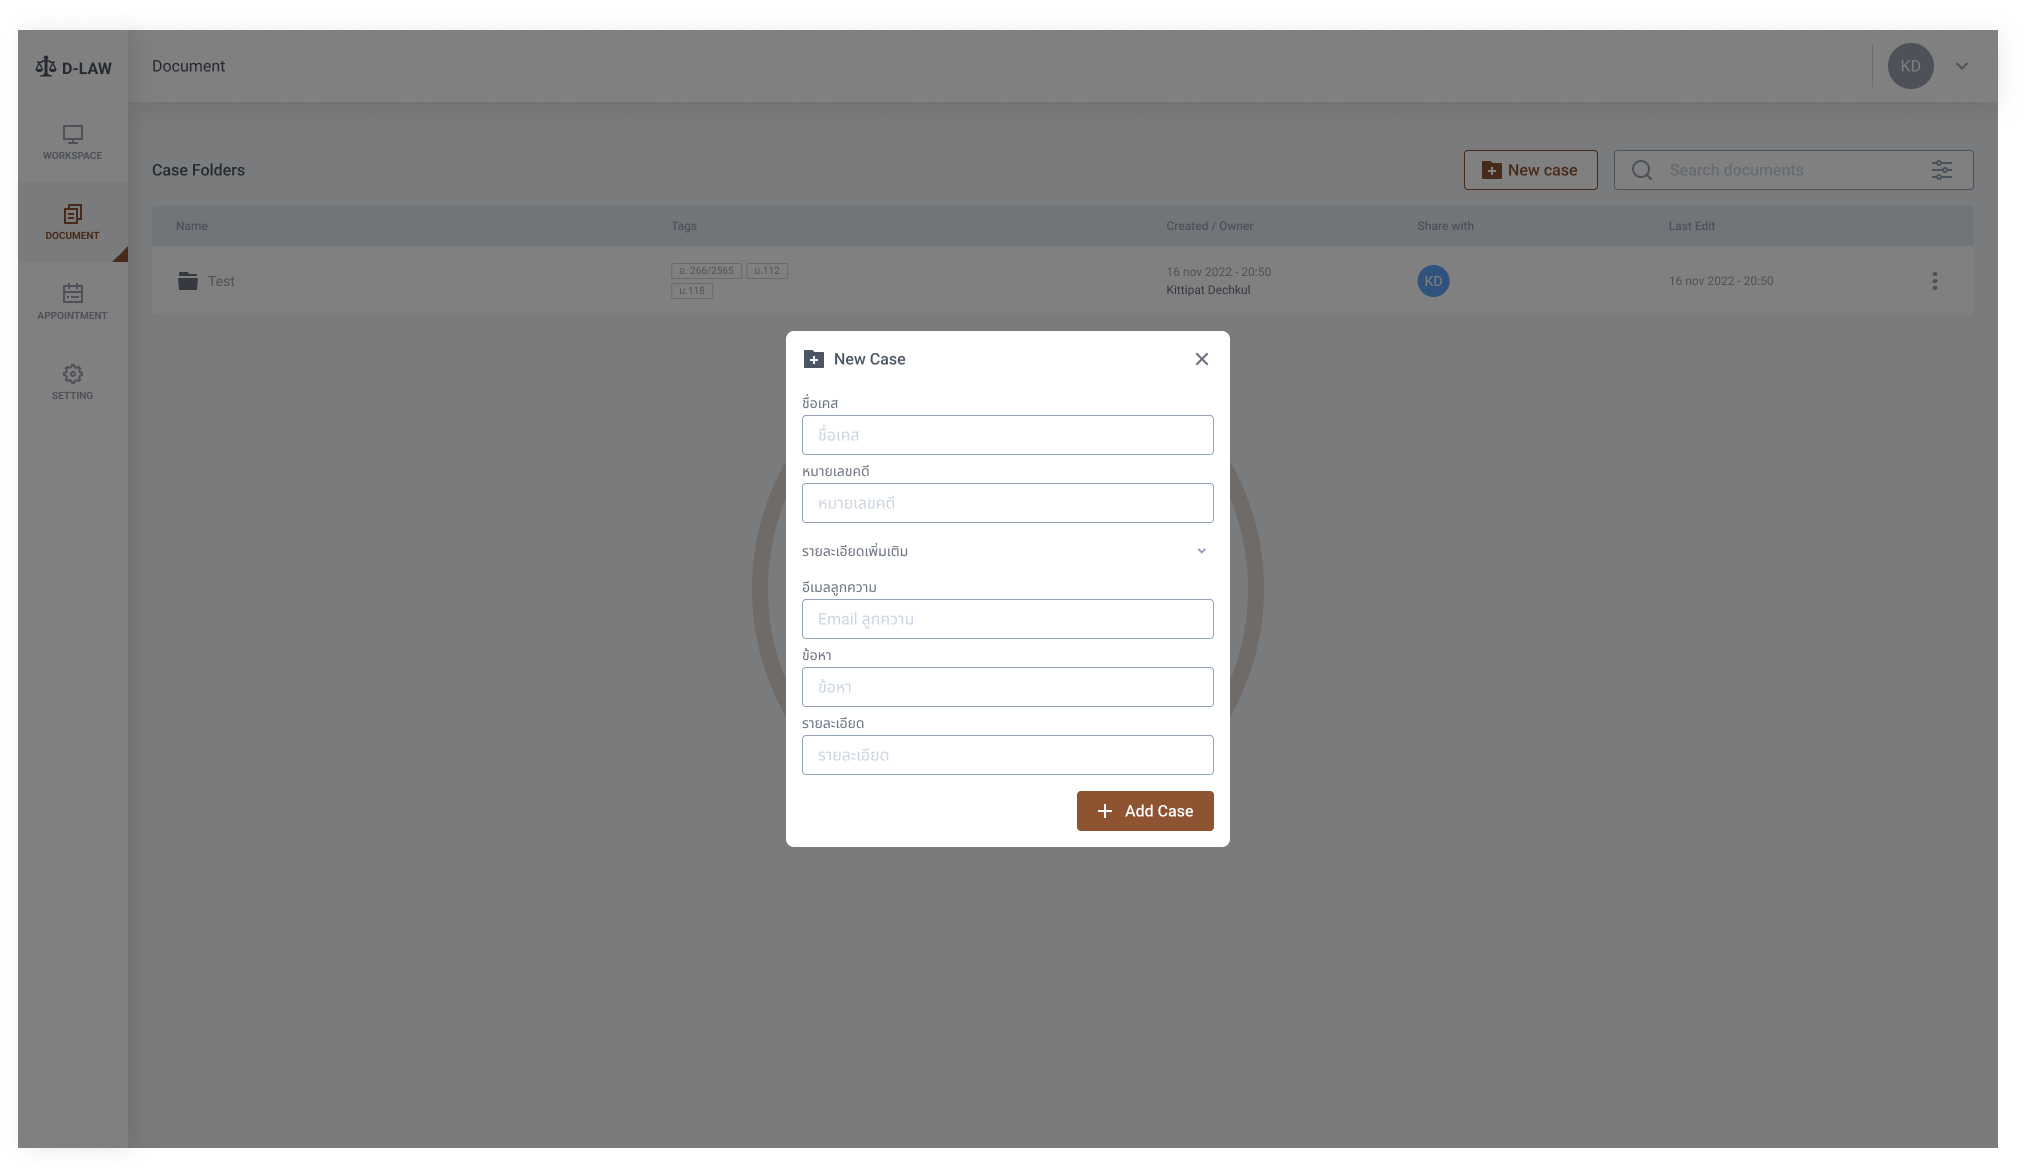
\includegraphics[width=13cm]{./assets/userinterface/new-case.png}
  \caption{รูปแสดงการออกแบบหน้าสร้างเคสใหม่}\label{fig:new-case}
\end{figure}

\begin{figure}[!h]\centering
  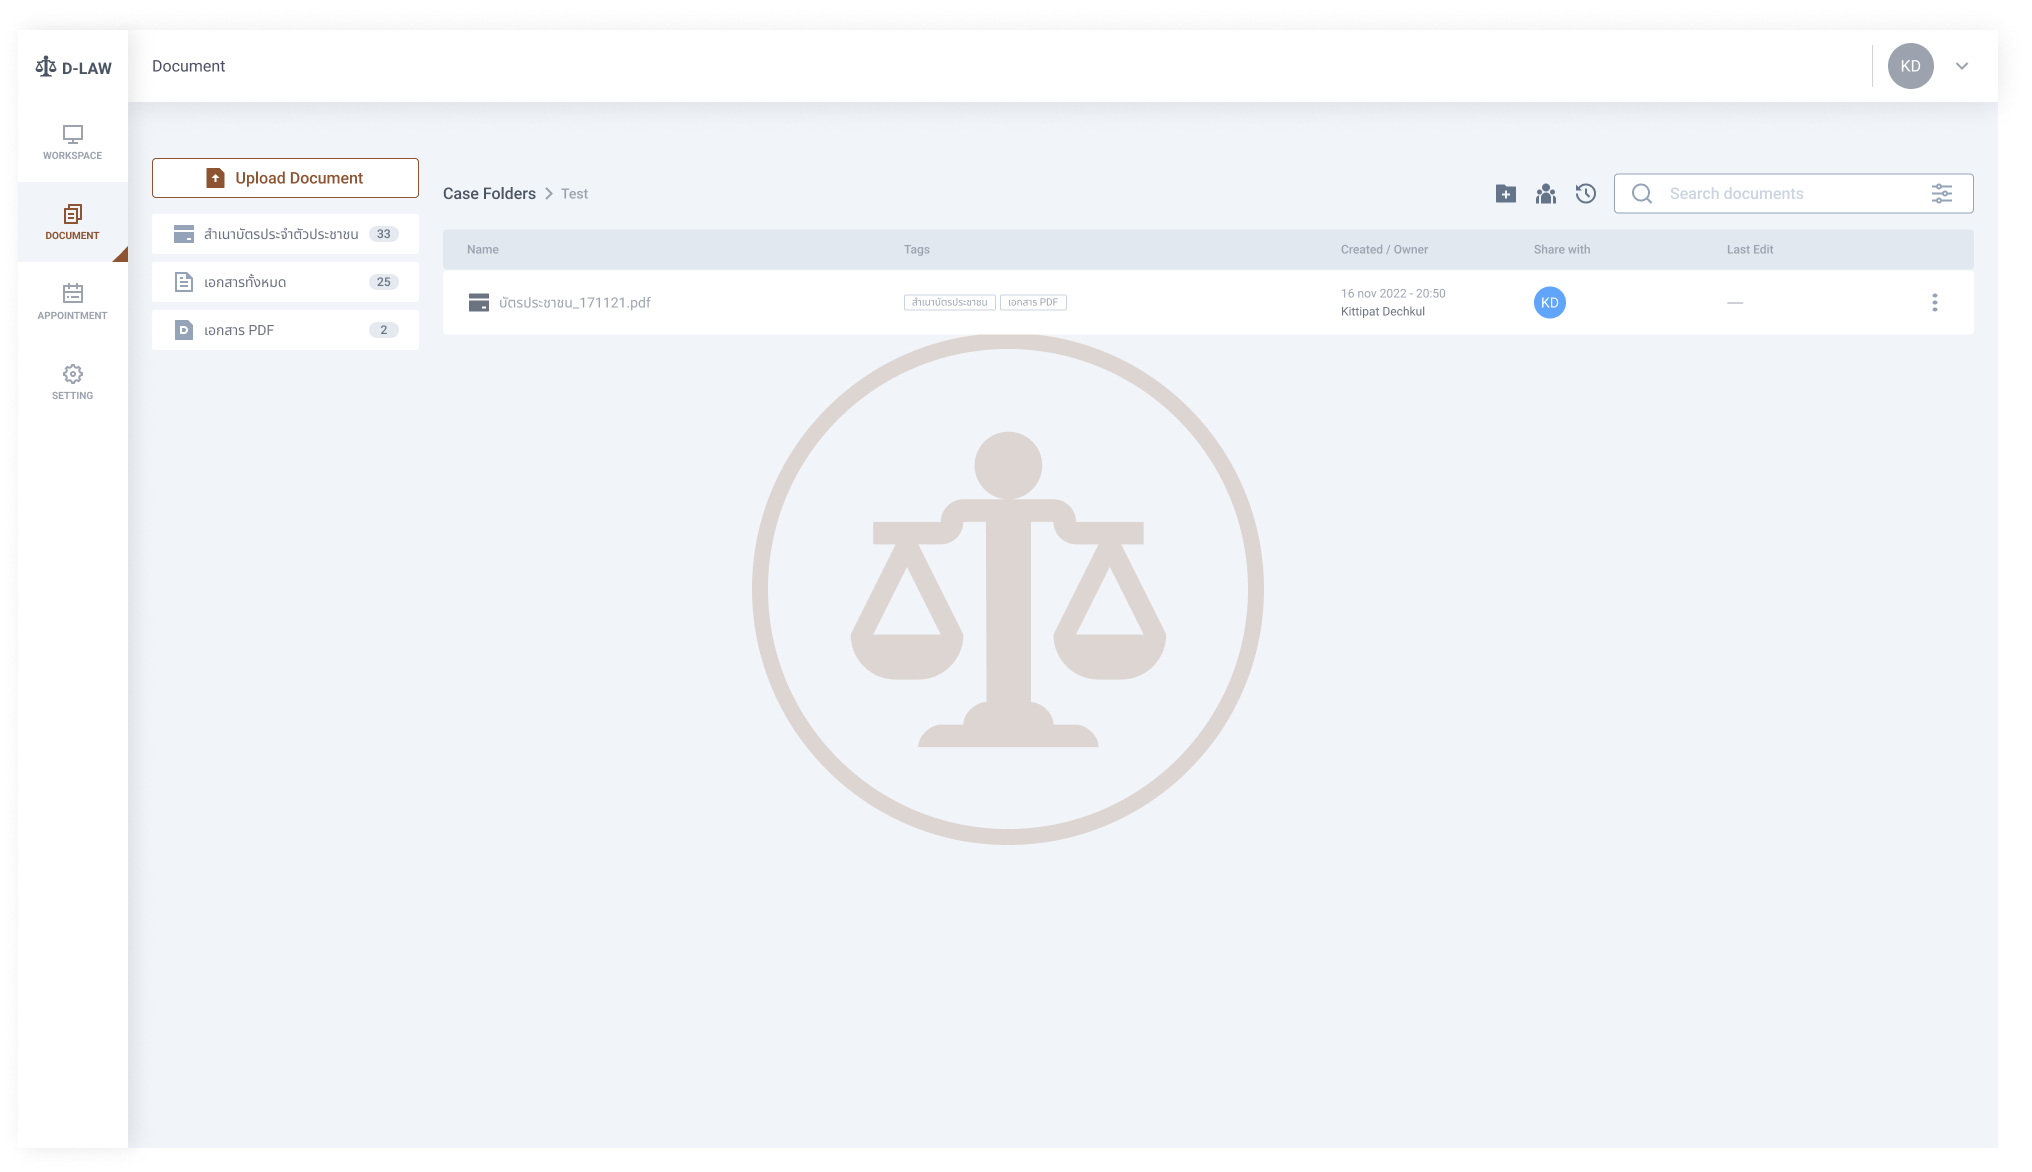
\includegraphics[width=13cm]{./assets/userinterface/document-list.png}
  \caption{รูปแสดงการออกแบบหน้าตารางแสดงไฟล์ต่าง ๆ}\label{fig:document-list}
\end{figure}

\begin{figure}[!h]\centering
  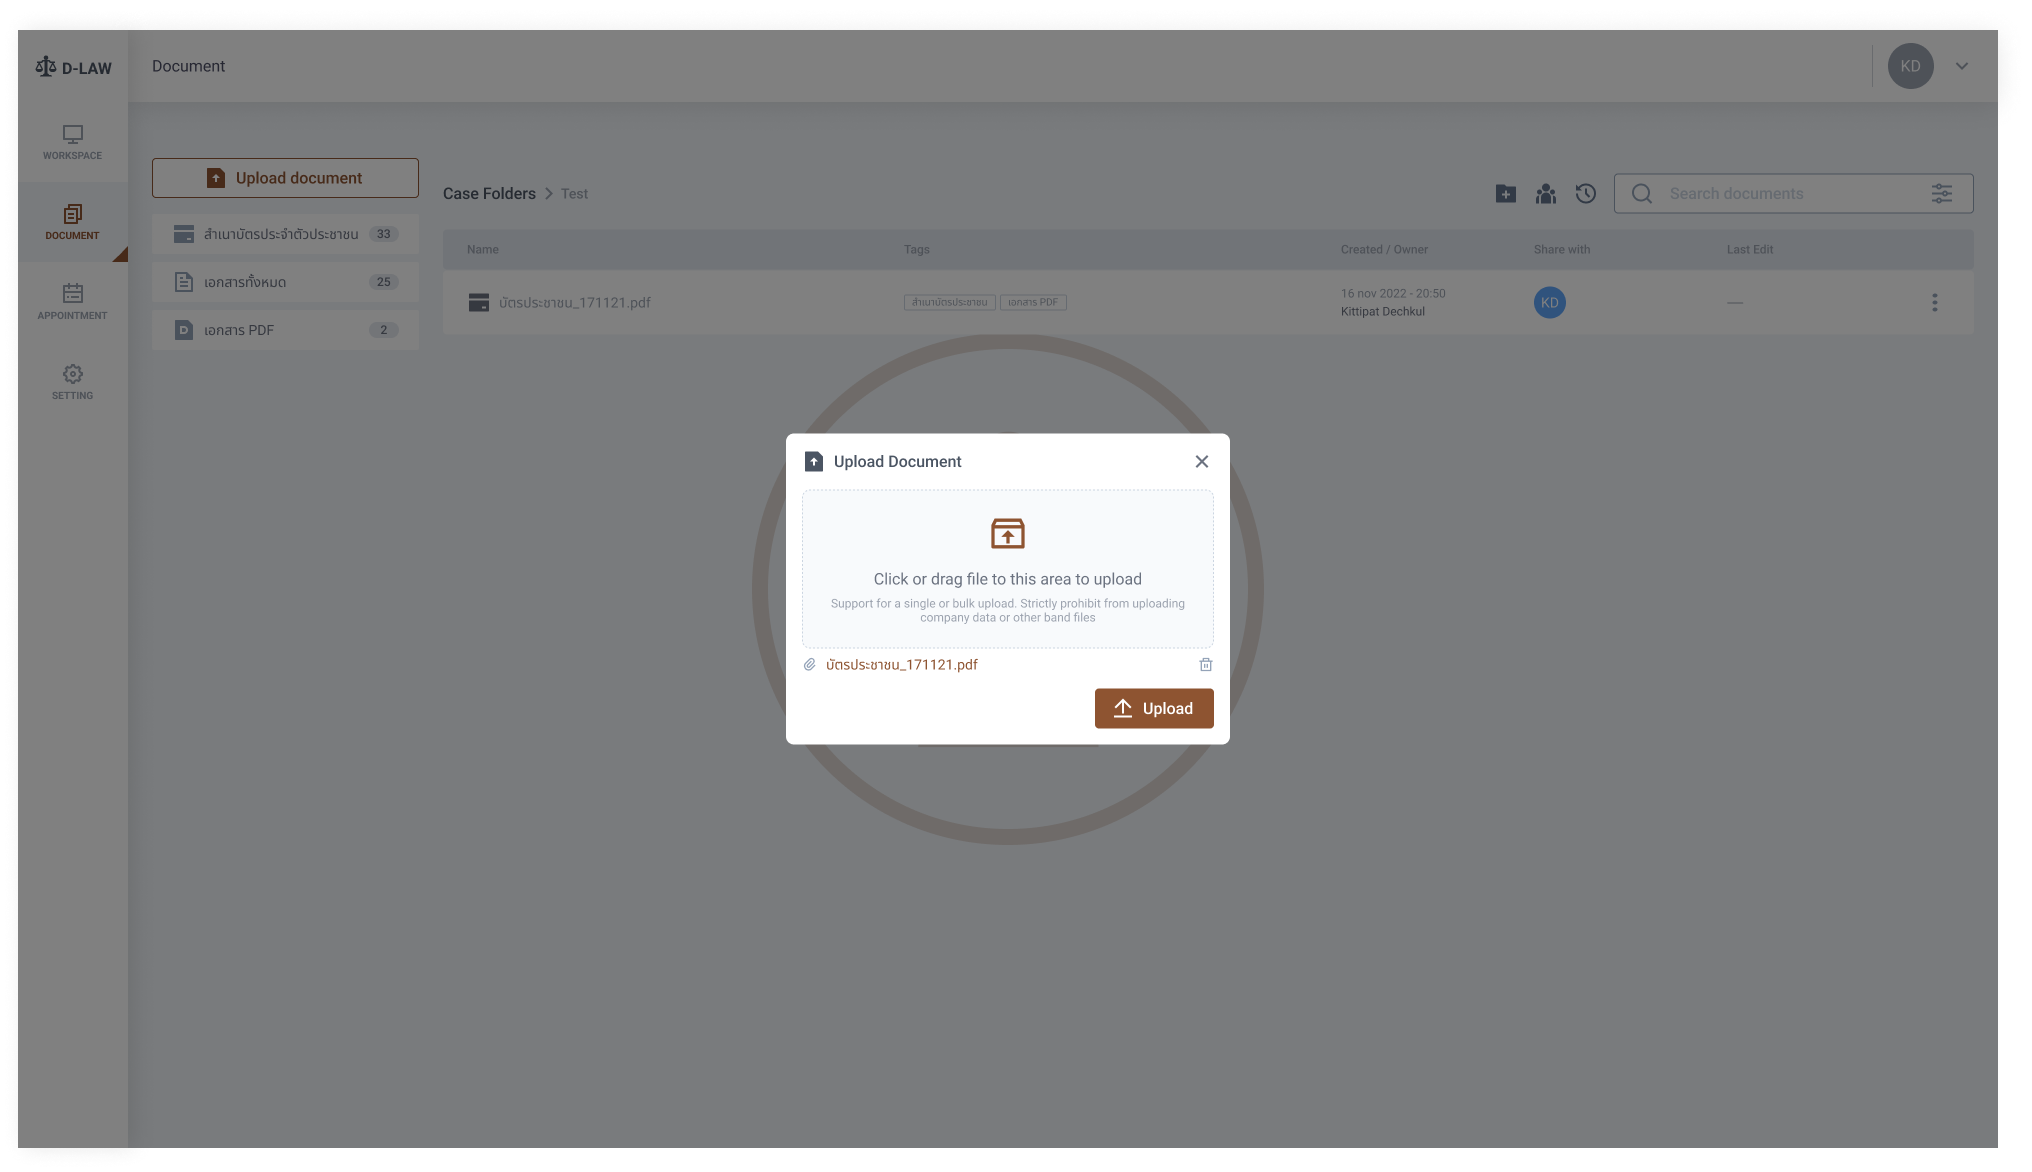
\includegraphics[width=13cm]{./assets/userinterface/upload-document.png}
  \caption{รูปแสดงการออกแบบหน้าอัพโหลดไฟล์}\label{fig:upload-document}
\end{figure}
\clearpage

\begin{figure}[!h]\centering
  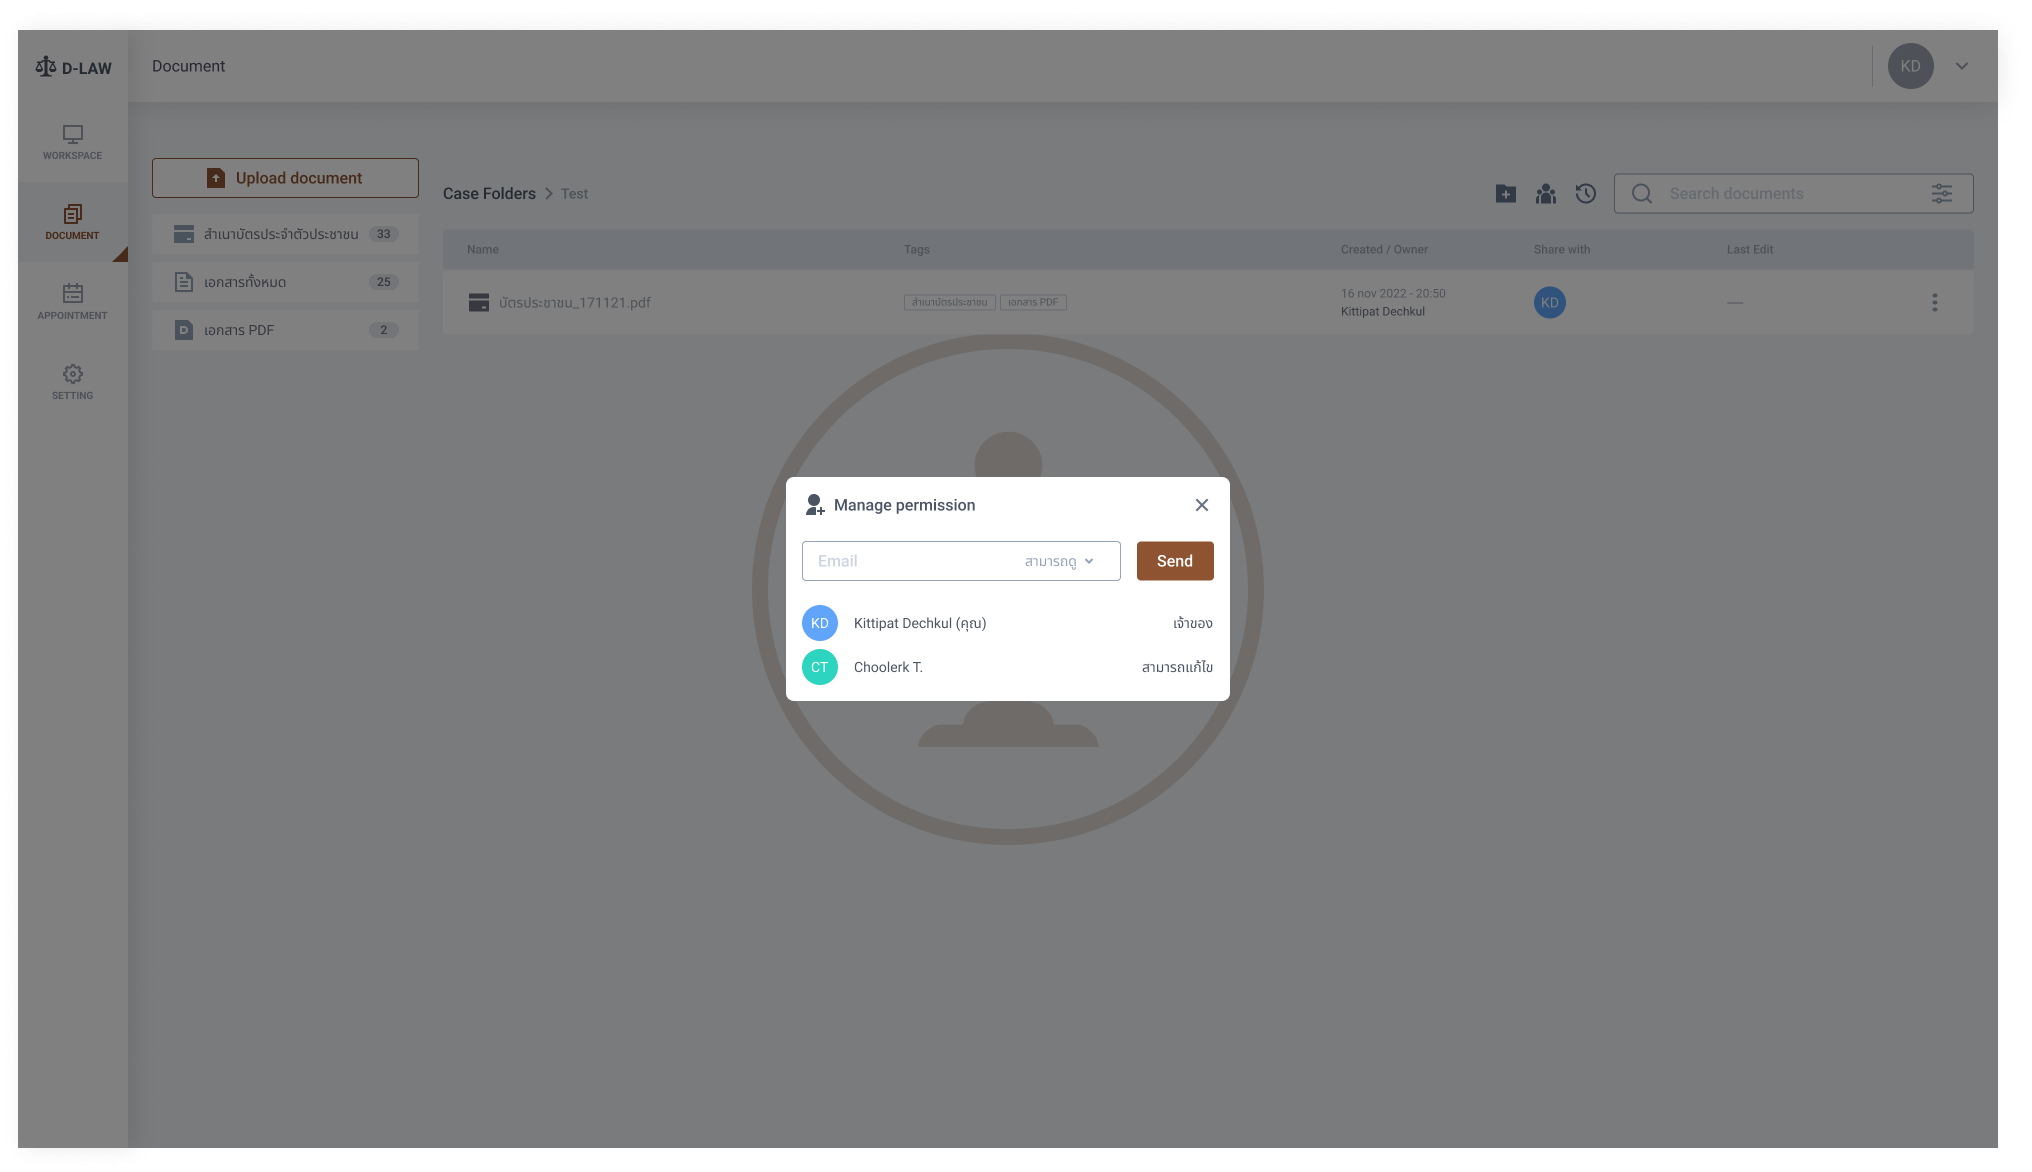
\includegraphics[width=13cm]{./assets/userinterface/folder-permission.png}
  \caption{รูปแสดงการออกแบบหน้าจัดการสิทธ์การเข้าถึงเคสโฟล์เดอร์}\label{fig:folder-permission}
\end{figure}

\begin{figure}[!h]\centering
  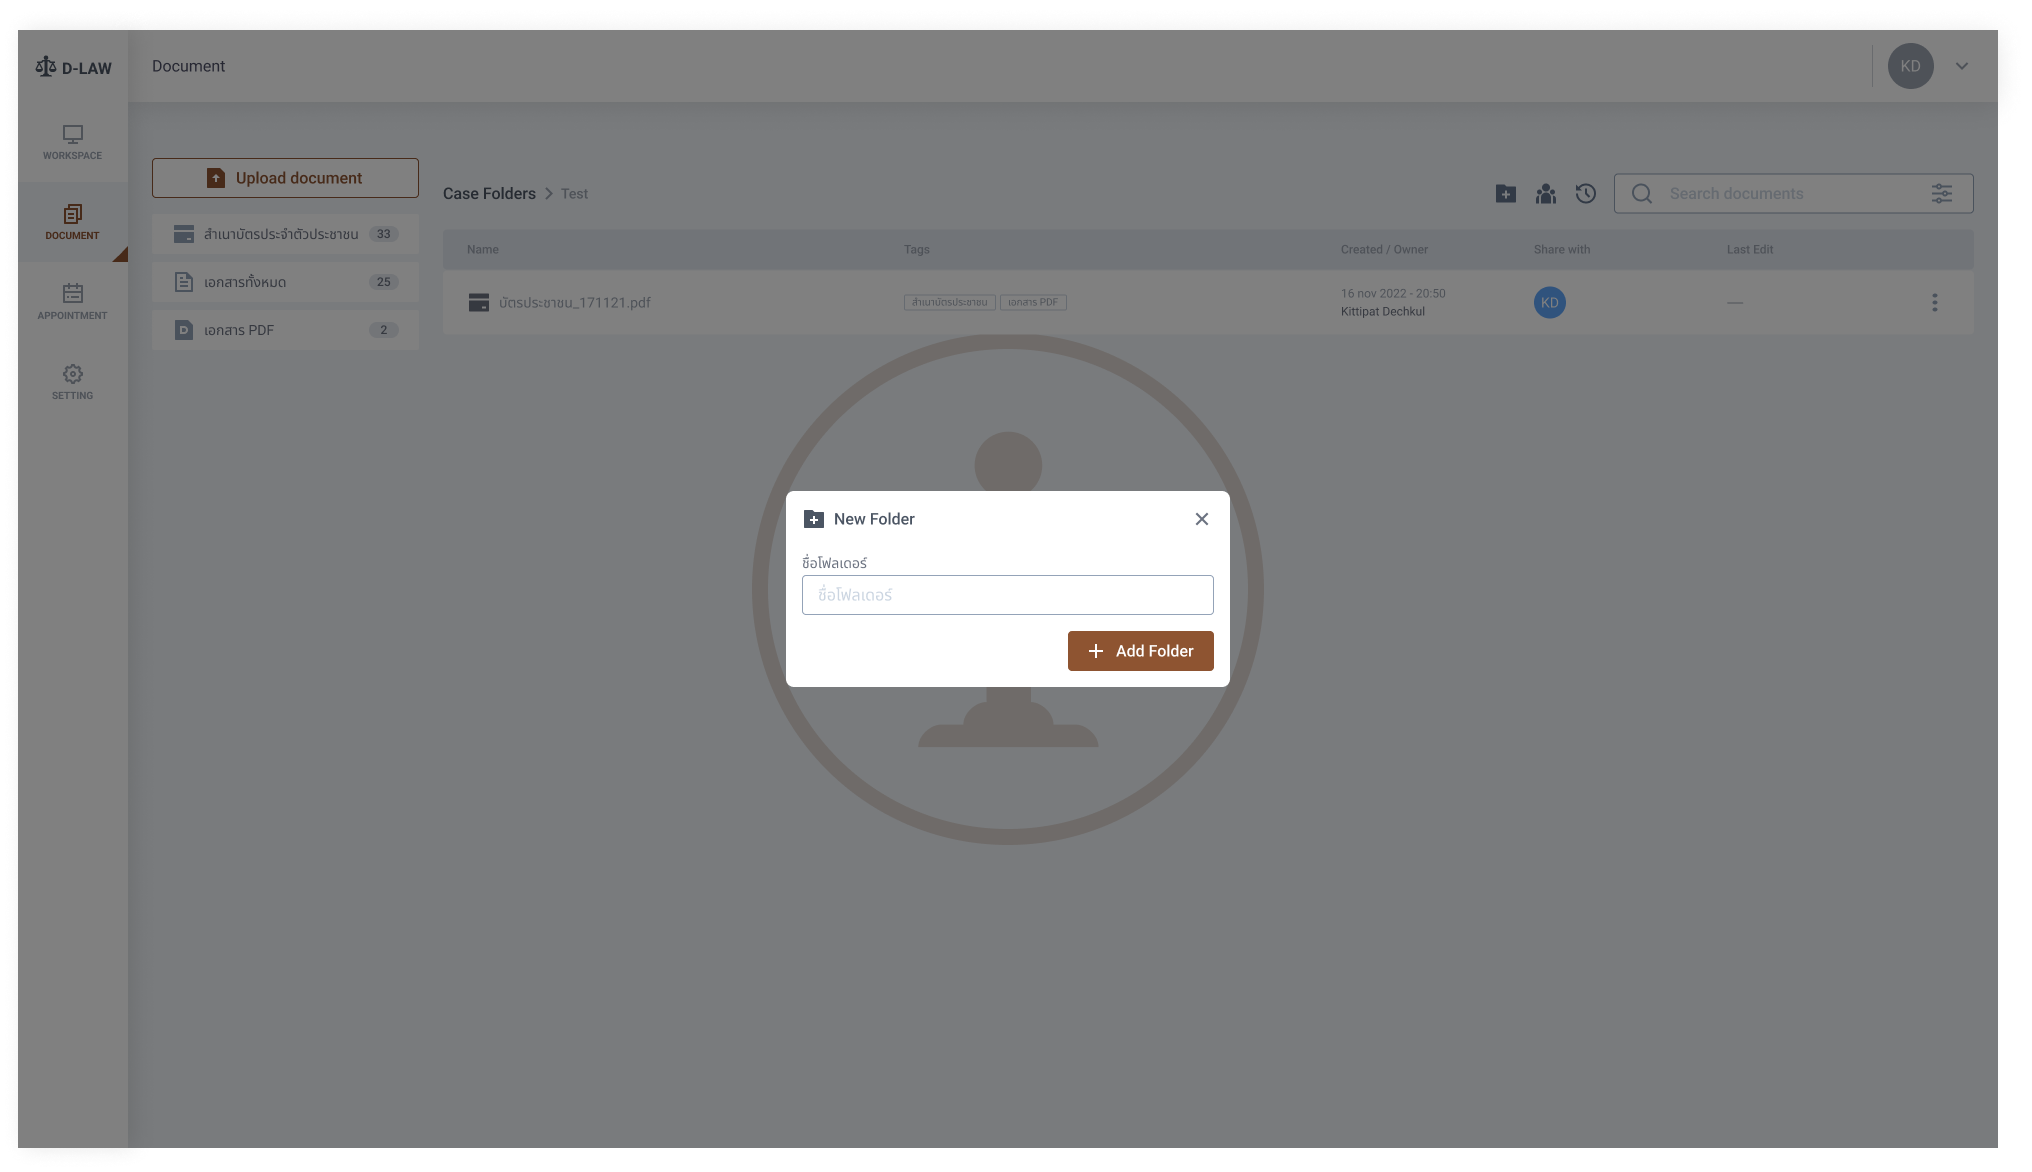
\includegraphics[width=13cm]{./assets/userinterface/create-new-folder.png}
  \caption{รูปแสดงการออกแบบหน้าสร้างโฟล์เดอร์ย่อยใหม่}\label{fig:create-new-folder}
\end{figure}

\begin{figure}[!h]\centering
  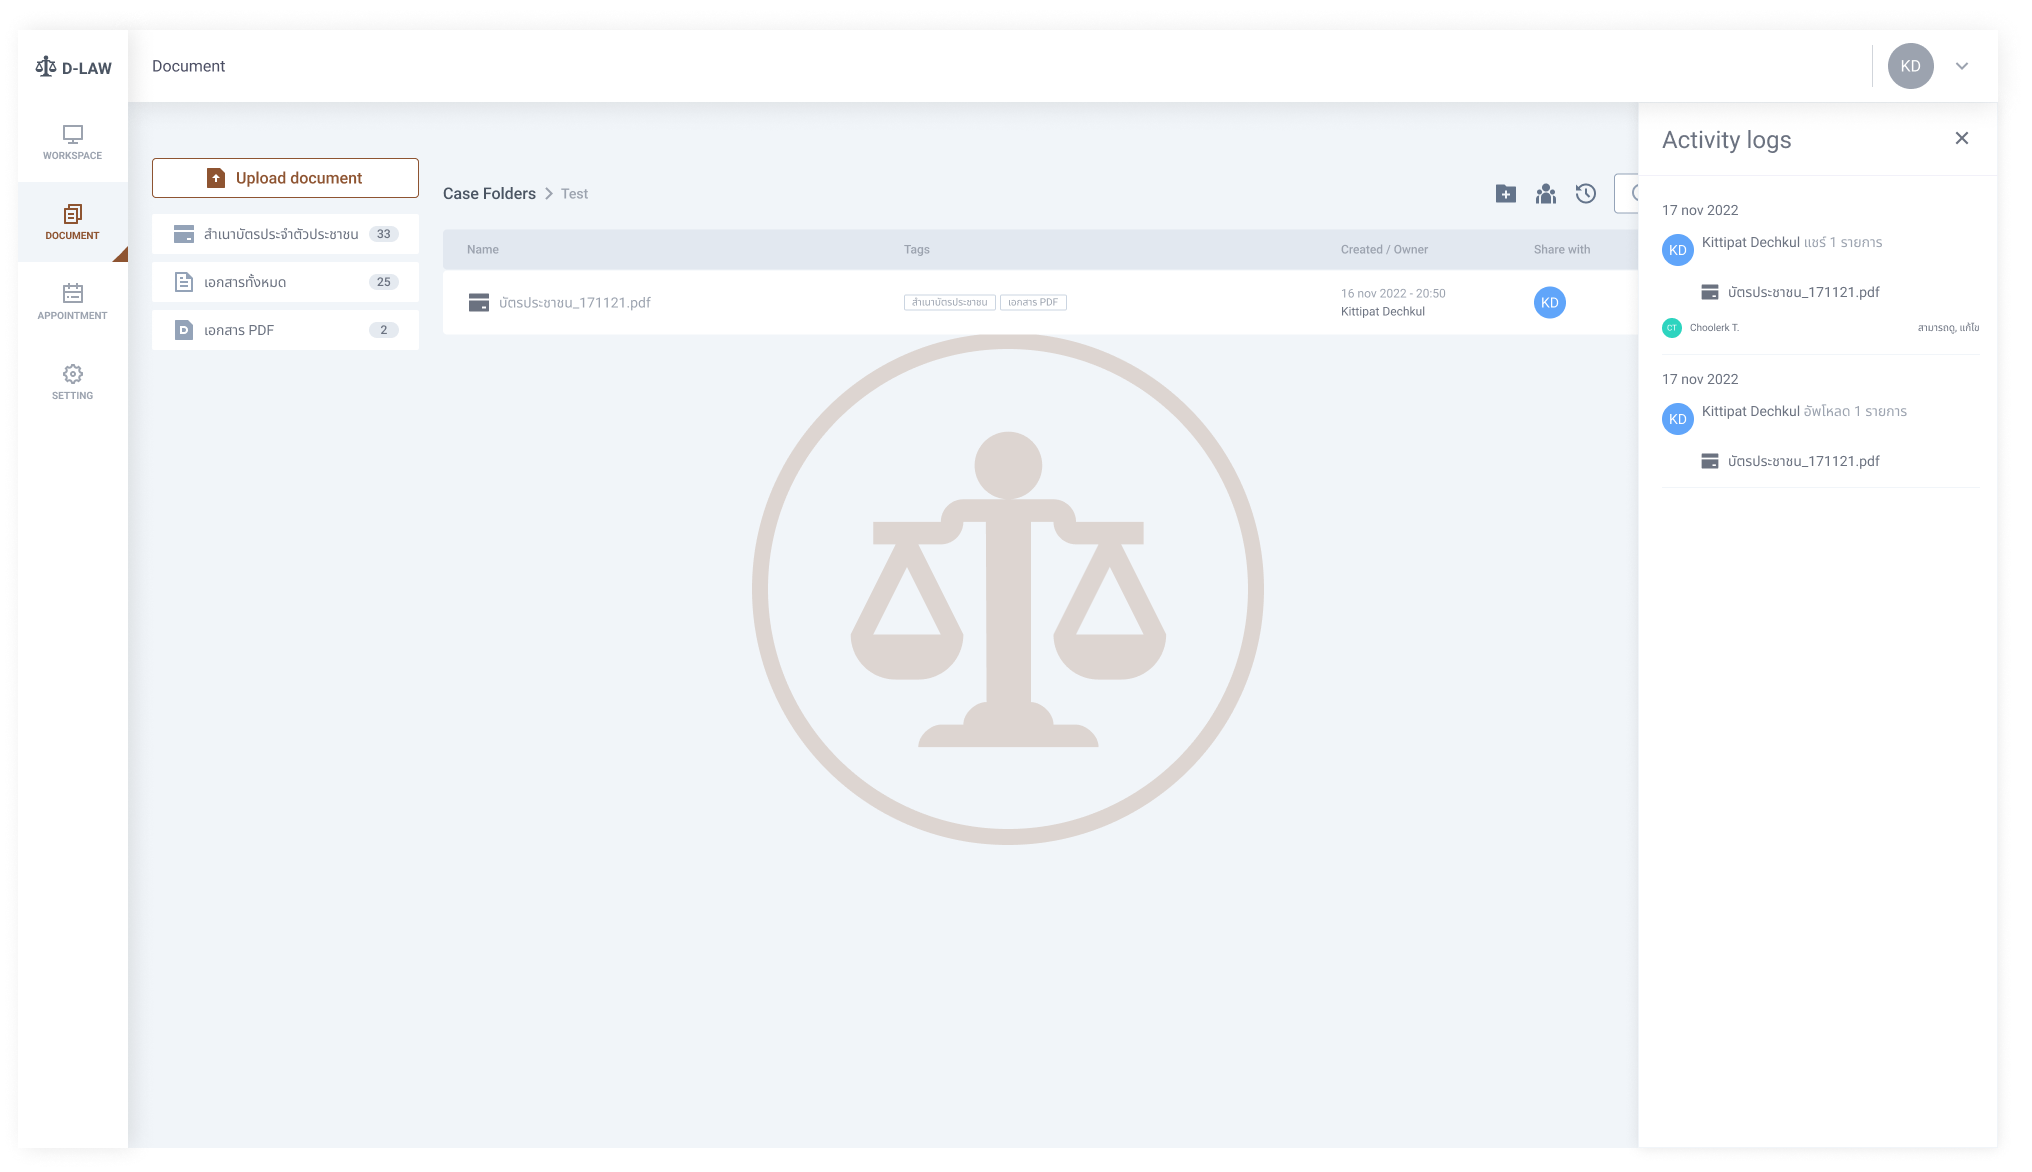
\includegraphics[width=13cm]{./assets/userinterface/activity-logs.png}
  \caption{รูปแสดงการออกแบบหน้าบันทึกกิจกรรมย้อนหลังของไฟล์}\label{fig:activity-logs}
\end{figure}

\newpage
\subsection{Preview file Page}
\hspace*{1cm} เป็นหน้าที่จะแสดง รายละเอียด รูปแบบเอกสาร และสามารถเผยแพร่เอกสารได้ ดังรูป \ref{fig:preview-file} - \ref{fig:public-document} ดังนี้
\begin{figure}[!h]\centering
  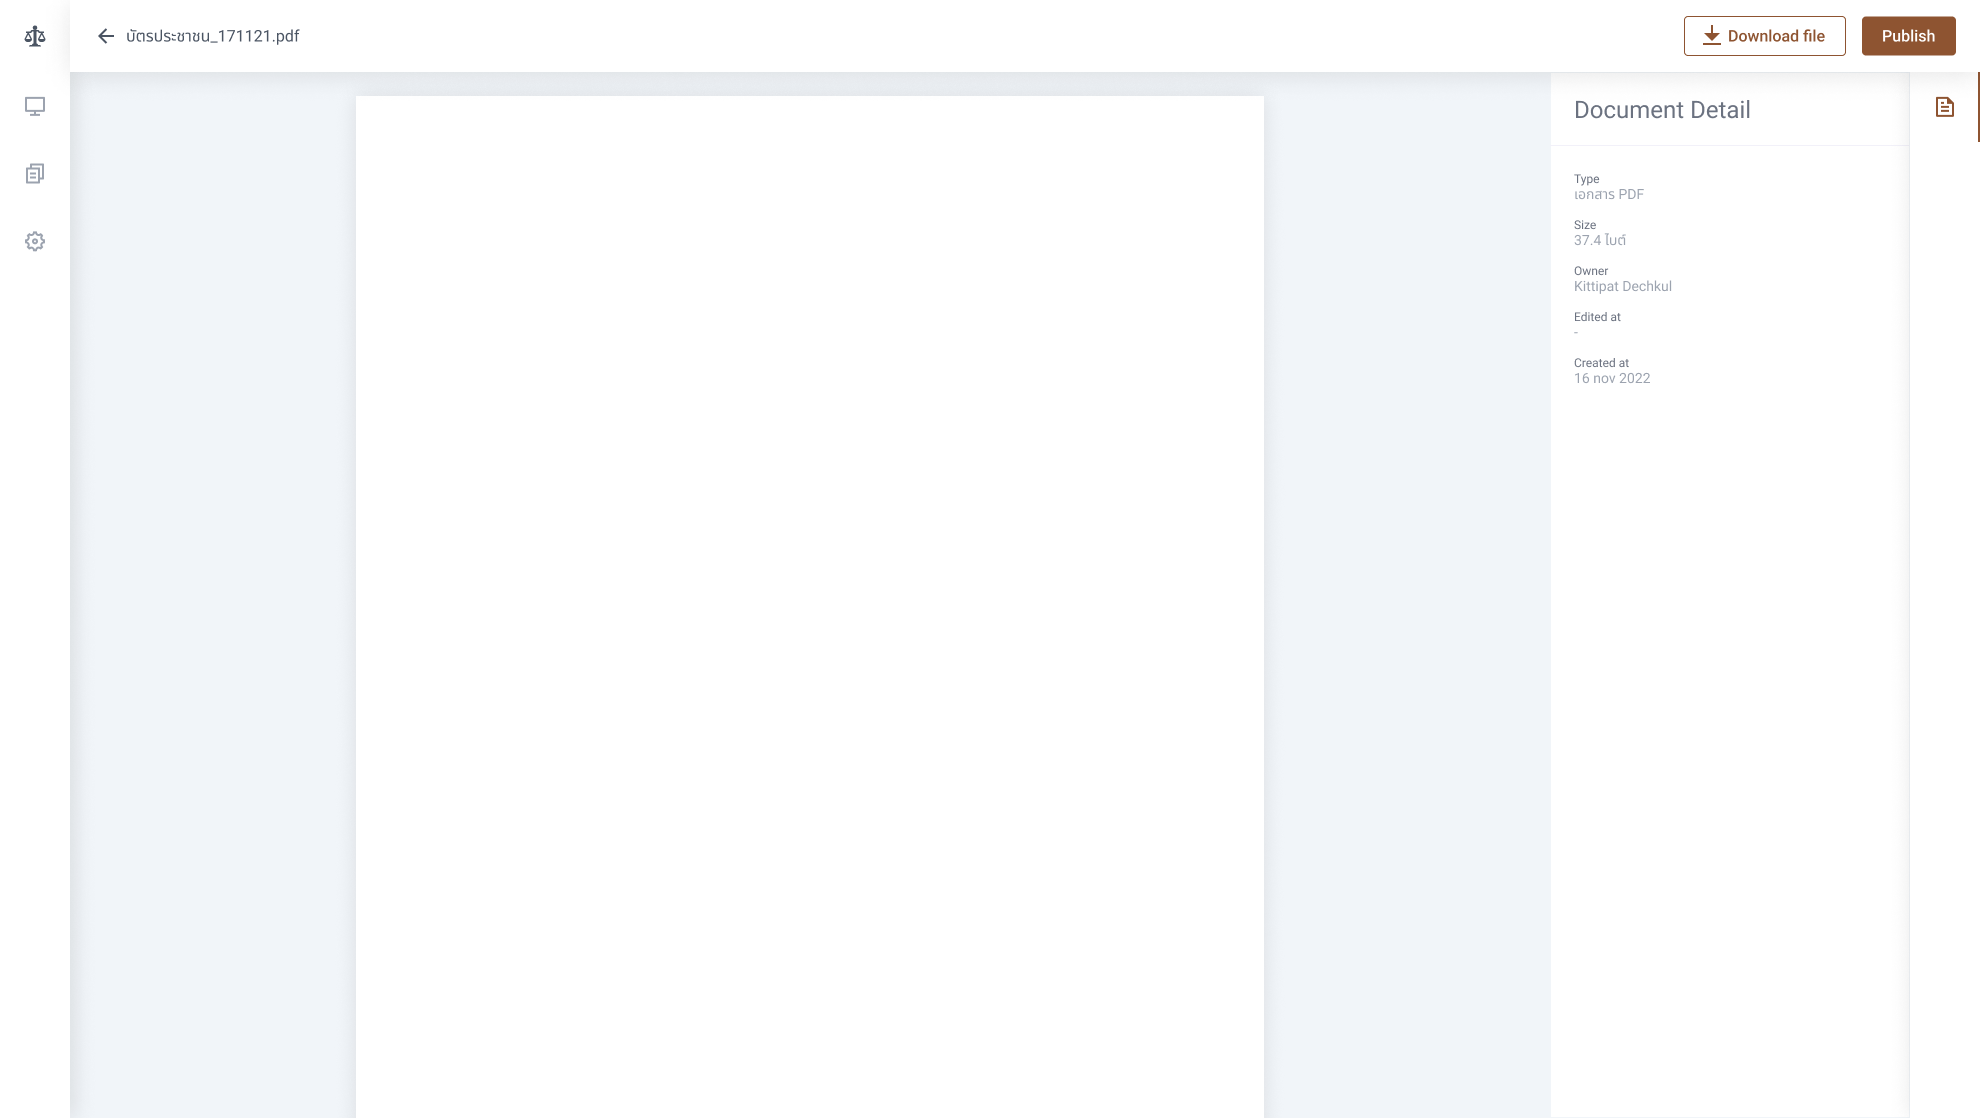
\includegraphics[width=13cm]{./assets/userinterface/preview-file.png}
  \caption{รูปแสดงการออกแบบหน้าแสดงรายระเอียดไฟล์เอกสาร}\label{fig:preview-file}
\end{figure}

\begin{figure}[!h]\centering
  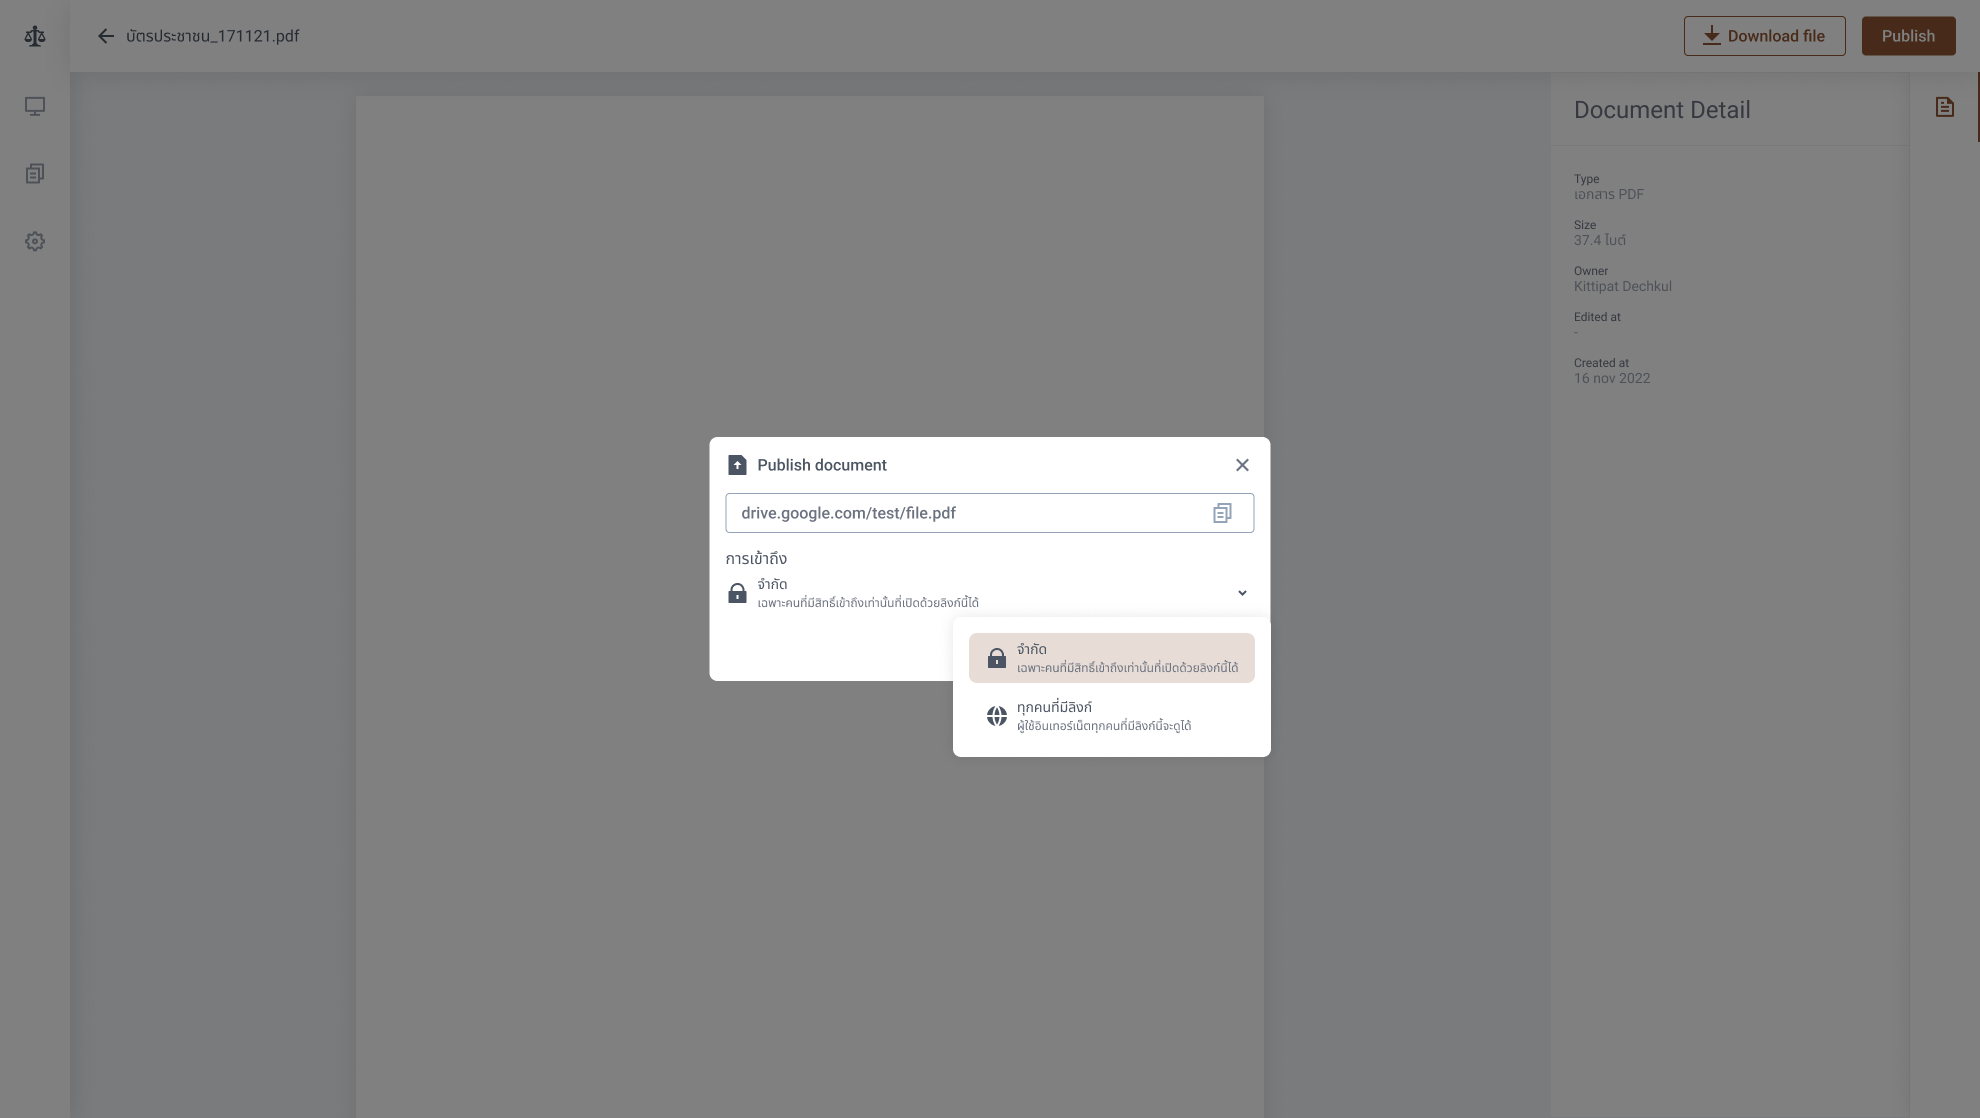
\includegraphics[width=13cm]{./assets/userinterface/public-document.png}
  \caption{รูปแสดงการออกแบบหน้าเผยแพร่ไฟล์เอกสาร}\label{fig:public-document}
\end{figure}

\newpage
\subsection{Appointment Page}
\hspace*{1cm} เป็นหน้าที่จะแสดงตารางนัดหมาย และสามารถส่งนัดหมายให้กับทนายคนอื่น ๆ และลูกความได้ ดังรูป \ref{fig:appointment} - \ref{fig:create-appointment-done} ดังนี้
\begin{figure}[!h]\centering
  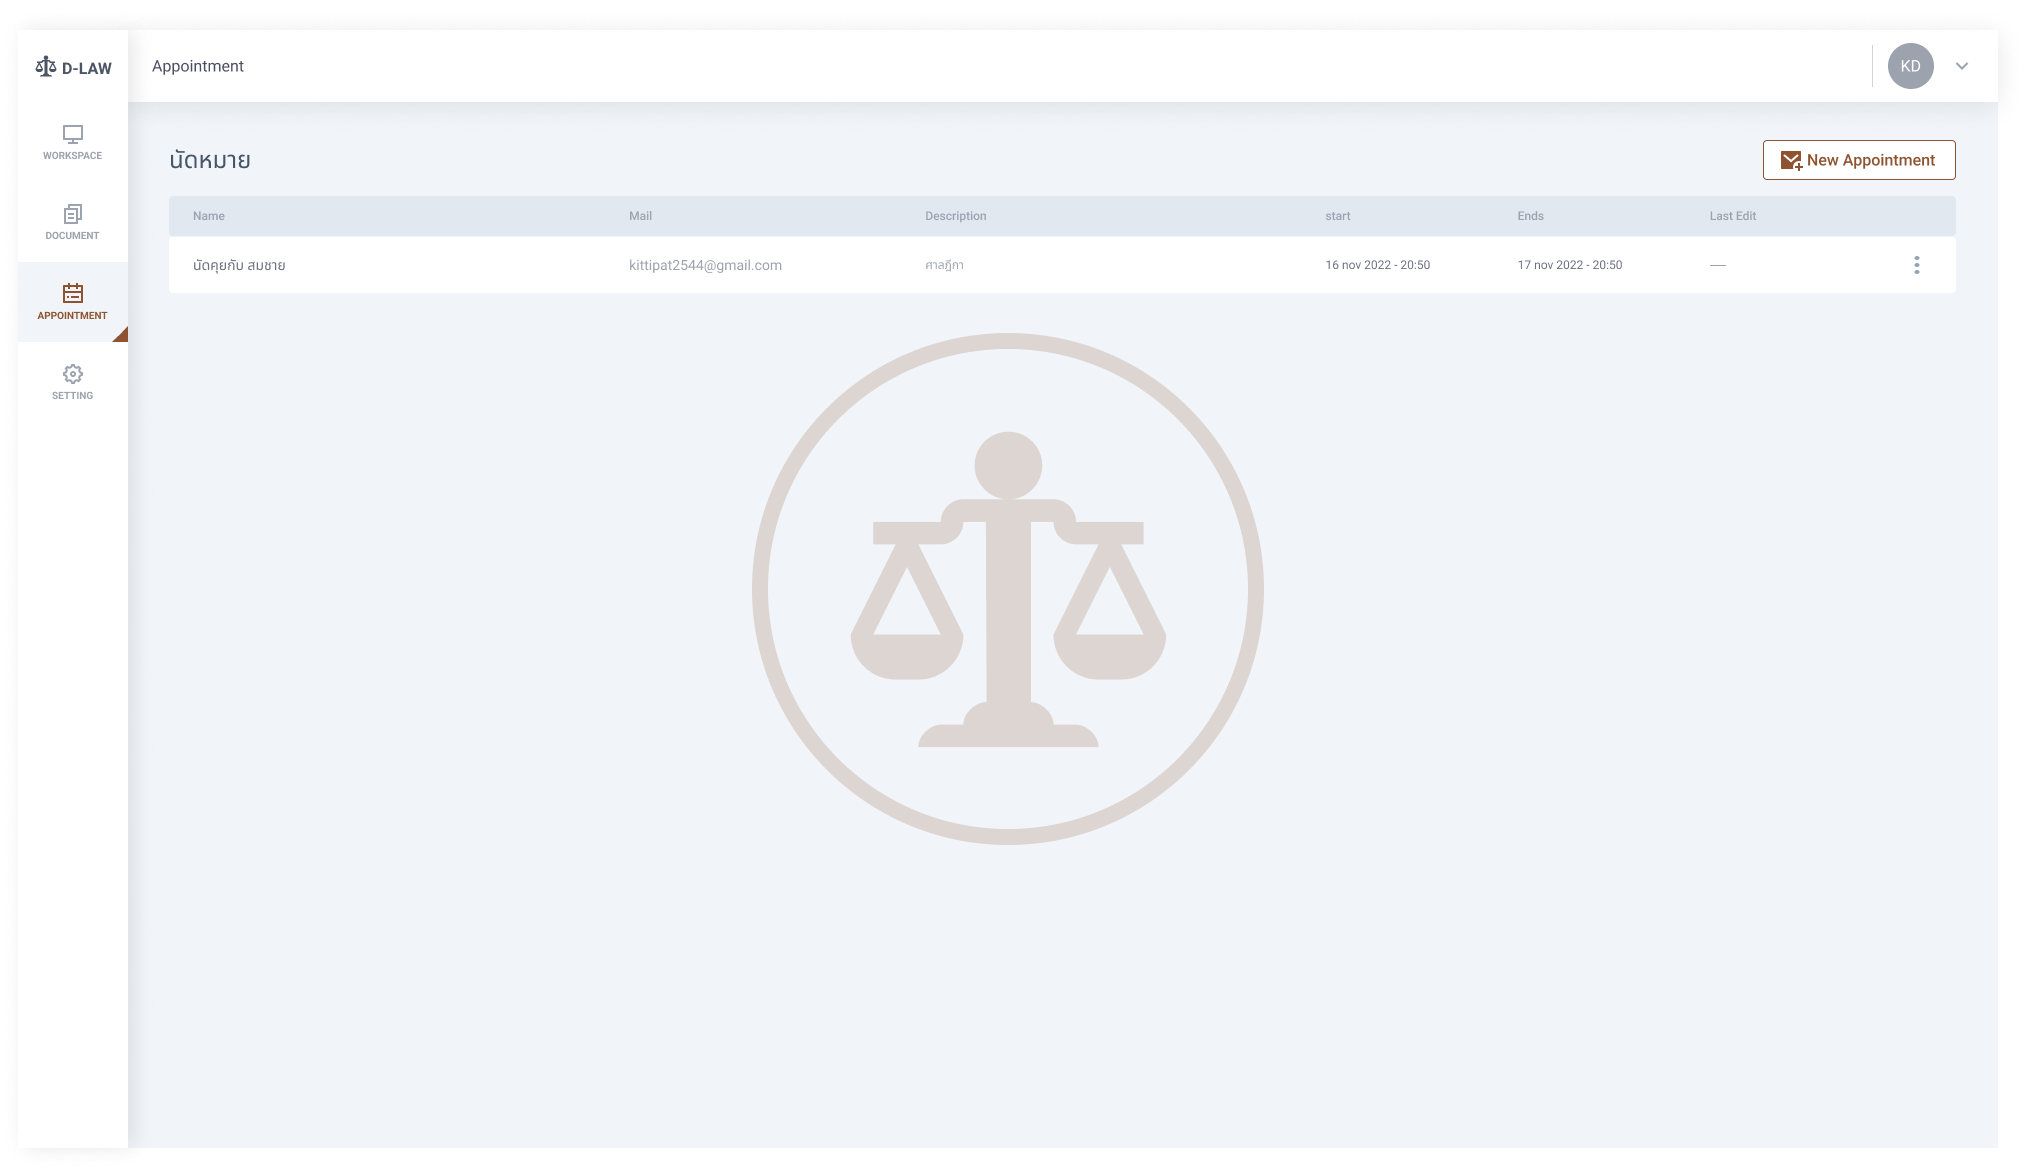
\includegraphics[width=13cm]{./assets/userinterface/appointment.png}
  \caption{รูปแสดงการออกแบบหน้าแสดงตารางนัดหมาย}\label{fig:appointment}
\end{figure}

\clearpage

\begin{figure}[!h]\centering
  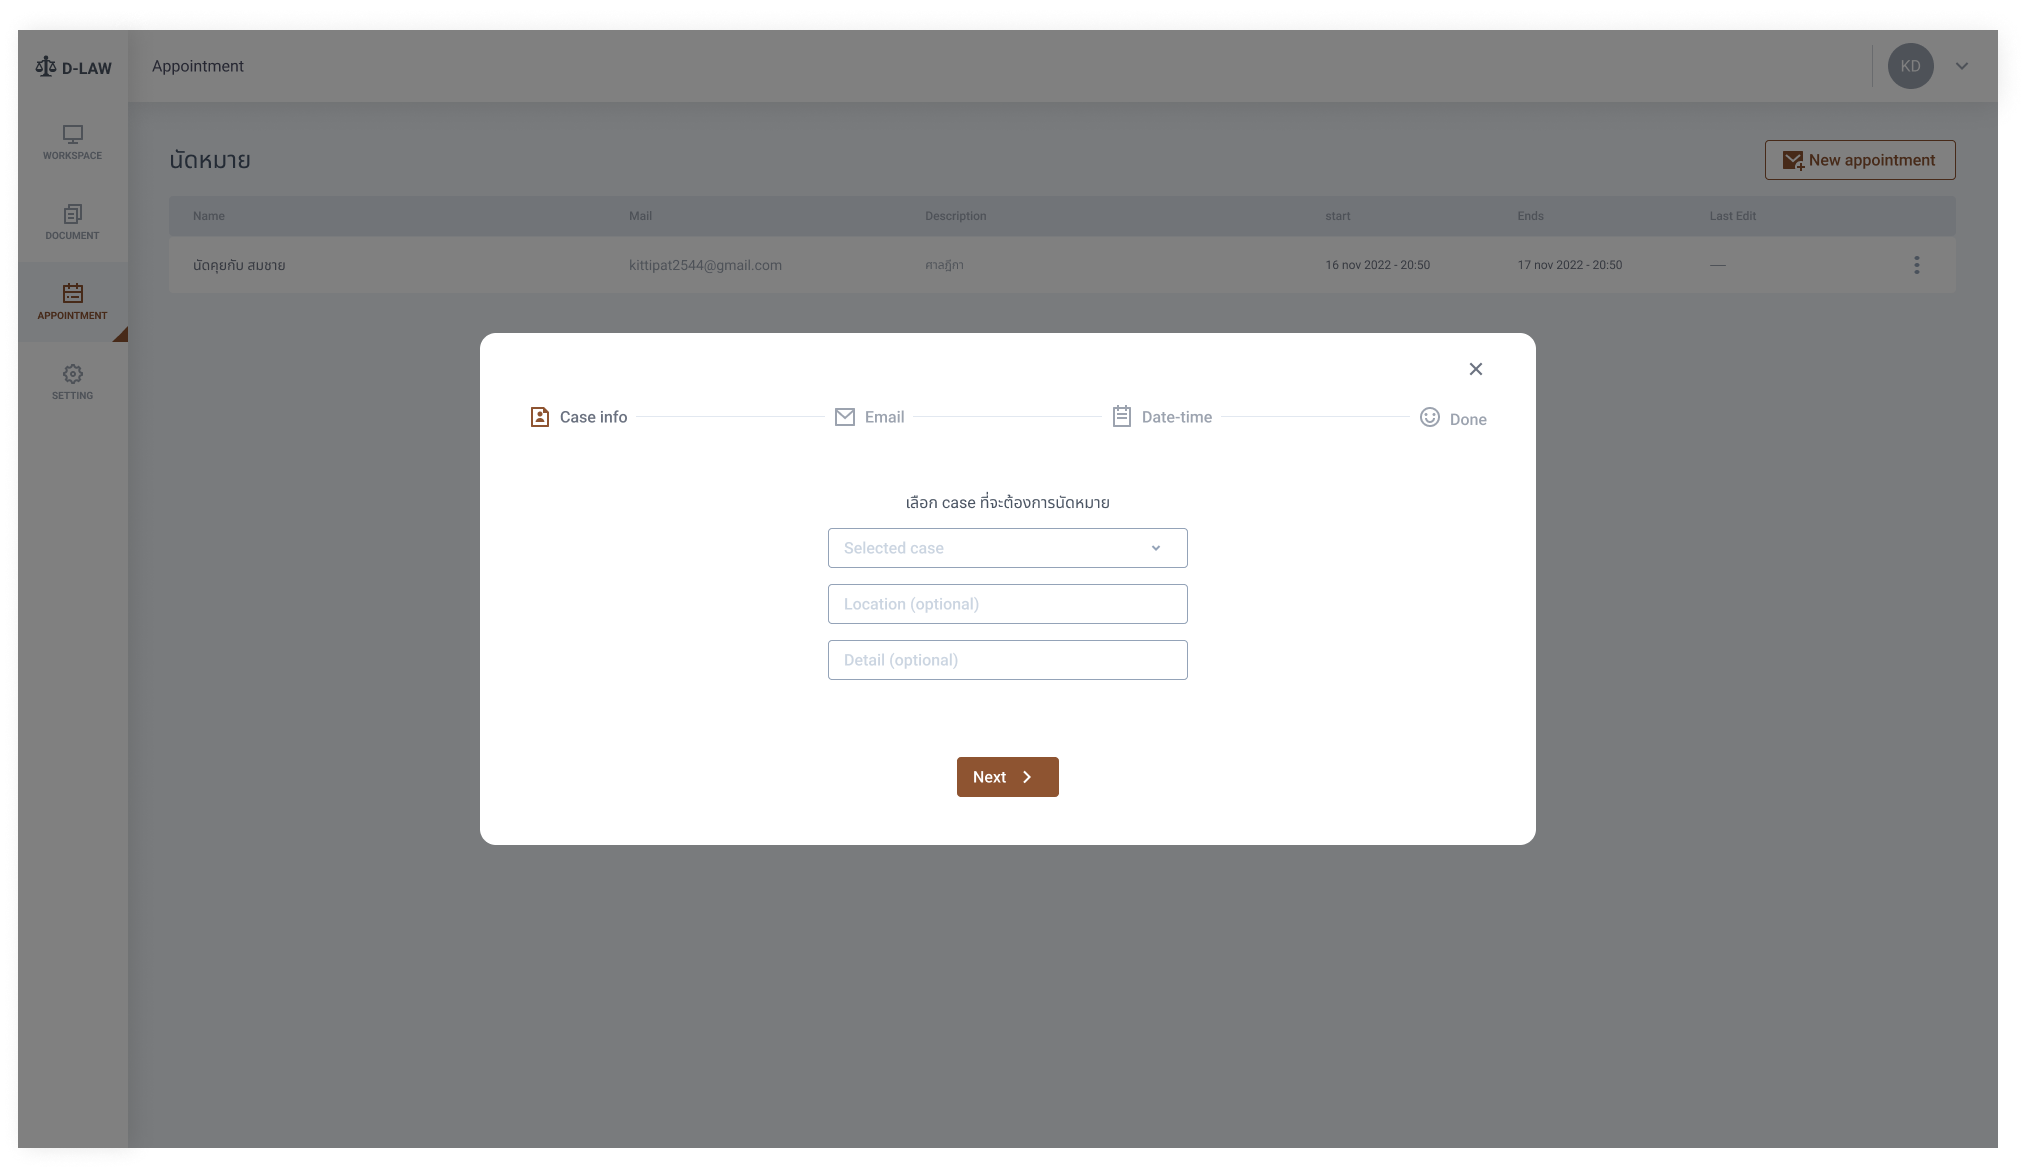
\includegraphics[width=13cm]{./assets/userinterface/create-appointment-info.png}
  \caption{รูปแสดงการออกแบบหน้าสร้างนัดหมาย ในขั้นตอนการกรอกข้อมูลนัดหมาย}\label{fig:create-appointment-info}
\end{figure}

\begin{figure}[!h]\centering
  \includegraphics[width=13cm]{./assets/userinterface/create-appointment-email.png}
  \caption{รูปแสดงการออกแบบหน้าสร้างนัดหมาย ในขั้นตอนการกรอกอีเมล}\label{fig:create-appointment-email}
\end{figure}

\begin{figure}[!h]\centering
  \includegraphics[width=13cm]{./assets/userinterface/create-appointment-datetime.png}
  \caption{รูปแสดงการออกแบบหน้าสร้างนัดหมาย ในขั้นตอนการกรอกวันเวลานัดหมาย}\label{fig:create-appointment-datetime}
\end{figure}

\begin{figure}[!h]\centering
  \includegraphics[width=13cm]{./assets/userinterface/create-appointment-done.png}
  \caption{รูปแสดงการออกแบบหน้าสร้างนัดหมาย ในขั้นตอนนัดหมายเสร็จสิ้น}\label{fig:create-appointment-done}
\end{figure}

\clearpage

\newpage
\subsection{Setting Page}
\hspace*{1cm} เป็นหน้าสำหรับแก้ไขข้อมูลโปรโฟล์ เปลี่ยนรหัสผ่าน และจัดการกับสมาชิกในองค์กรได้ ดังรูป \ref{fig:setting-myprofile} - \ref{fig:setting-create-user} ดังนี้

\begin{figure}[!h]\centering
  \includegraphics[width=13cm]{./assets/userinterface/setting-myprofile.png}
  \caption{รูปแสดงการออกแบบหน้าแก้ไขโปรฟล์ และเปลี่ยนรหัสผ่าน }\label{fig:setting-myprofile}
\end{figure}

\begin{figure}[!h]\centering
  \includegraphics[width=13cm]{./assets/userinterface/setting-manage-user.png}
  \caption{รูปแสดงการออกแบบหน้าแสดงตารางผู้ใช้งาน}\label{fig:setting-manage-user}
\end{figure}

\begin{figure}[!h]\centering
  \includegraphics[width=13cm]{./assets/userinterface/setting-create-user.png}
  \caption{รูปแสดงการออกแบบหน้าเพิ่มผู้ใช้งานใหม่}\label{fig:setting-create-user}
\end{figure}


%%%%%%%%%%%%%%%%%%%%%%%%%%%%%%%%%%%%%%%%%%%%%%%%%%%%%%%%%%%%
%%%%%%%%%%%%%%%%%%%%%%% CHAPTER4 %%%%%%%%%%%%%%%%%%%%%%%%%%%
%%%%%%%%%%%%%%%%%%%%%%%%%%%%%%%%%%%%%%%%%%%%%%%%%%%%%%%%%%%%
\chapter{ผลการดำเนินงาน}

You can title this chapter as \textbf{Preliminary Results} ผลการดำเนินงานเบื้องต้น or \textbf{Work Progress} ความก้าวหน้าโครงงาน for the progress reports. Present implementation or experimental results here and discuss them.
ใส่เฉพาะหัวข้อที่เกี่ยวข้องกับงานที่ทำ 

\section{ประสิทฺธิภาพการทำงานของระบบ} 
\section{ความพึงพอใจการใช้งาน}
\section{การวิเคราะห์ข้อมูลและผลการทดลอง}

%%%%%%%%%%%%%%%%%%%%%%%%%%%%%%%%%%%%%%%%%%%%%%%%%%%%%%%%%%%%
%%%%%%%%%%%%%%%%%%%%%%% CHAPTER5 %%%%%%%%%%%%%%%%%%%%%%%%%%%
%%%%%%%%%%%%%%%%%%%%%%%%%%%%%%%%%%%%%%%%%%%%%%%%%%%%%%%%%%%%
\chapter{บทสรุป}

This chapter is optional for proposal and progress reports but 
is required for the final report.

\section{สรุปผลโครงงาน}
สรุปว่าโครงงานบรรลุตามวัตถุประสงค์ที่ตั้งไว้หรือไม่ อย่างไร 

\section{ปัญหาที่พบและการแก้ไข}
State your problems and how you fixed them.

\section{ข้อจำกัดและข้อเสนอแนะ}
ข้อจำกัดของโครงงาน What could be done in the future to make your projects better.

%%%%%%%%%%%%%%%%%%%%%%%%%%%%%%%%%%%%%%%%%%%%%%%%%%%%%%%%%%%%%%%
%%%%%%%%%%%%%%%%%%%% Bibliography %%%%%%%%%%%%%%%%%%%%%%%%%%%%%
%%%%%%%%%%%%%%%%%%%%%%%%%%%%%%%%%%%%%%%%%%%%%%%%%%%%%%%%%%%%%%%

%%%% Comment this in your report to show only references you have
%%%% cited. Otherwise, all the references below will be shown.
%\nocite{*}
%% Use the kmutt.bst for bibtex bibliography style 
%% You must have cpe.bib and string.bib in your current directory.
%% You may go to file .bbl to manually edit the bib items.

\makeatletter
\g@addto@macro{\UrlBreaks}{\UrlOrds}
\makeatother

\bibliographystyle{kmutt}
\bibliography{string,cpe}

%%%%%%%%%%%%%%%%%%%%%%%%%%%%%%%%%%%%%%%%%%%%%%%%%%%%%%%%%%%%%%%
%%%%%%%%%%%%%%%%%%%%%%%% Appendix %%%%%%%%%%%%%%%%%%%%%%%%%%%%%
%%%%%%%%%%%%%%%%%%%%%%%%%%%%%%%%%%%%%%%%%%%%%%%%%%%%%%%%%%%%%%%
\appendix{ชื่อภาคผนวกที่ 1}
\noindent{\large\bf ใส่หัวข้อตามความเหมาะสม} \\





\end{document}
